\documentclass{article}

% if you need to pass options to natbib, use, e.g.:
%     \PassOptionsToPackage{numbers, compress}{natbib}
% before loading neurips_2026

% The authors should use one of these tracks.
% Before accepting by the NeurIPS conference, select one of the options below.
% 0. "default" for submission
\usepackage{neurips_2026}
% the "default" option is equal to the "main" option, which is used for the Main Track with double-blind reviewing.
% 1. "main" option is used for the Main Track
%  \usepackage[main]{neurips_2026}
% 2. "position" option is used for the Position Paper Track
%  \usepackage[position]{neurips_2026}
% 3. "eandd" option is used for the Evaluations & Datasets Track
% \usepackage[eandd]{neurips_2026}
% if you need to opt-in for a single-blind submission in the E&D track:
%\usepackage[eandd, nonanonymous]{neurips_2026}
% 4. "creativeai" option is used for the Creative AI Track
%  \usepackage[creativeai]{neurips_2026}
% 5. "sglblindworkshop" option is used for the Workshop with single-blind reviewing
% \usepackage[sglblindworkshop]{neurips_2026}
% 6. "dblblindworkshop" option is used for the Workshop with double-blind reviewing
%  \usepackage[dblblindworkshop]{neurips_2026}

% After being accepted, the authors should add "final" behind the track to compile a camera-ready version.
% 1. Main Track
% \usepackage[main, final]{neurips_2026}
% 2. Position Paper Track
%  \usepackage[position, final]{neurips_2026}
% 3. Evaluations & Datasets Track
% \usepackage[eandd, final]{neurips_2026}
% 4. Creative AI Track
%  \usepackage[creativeai, final]{neurips_2026}
% 5. Workshop with single-blind reviewing
%  \usepackage[sglblindworkshop, final]{neurips_2026}
% 6. Workshop with double-blind reviewing
%  \usepackage[dblblindworkshop, final]{neurips_2026}
% Note. For the workshop paper template, both \title{} and \workshoptitle{} are required, with the former indicating the paper title shown in the title and the latter indicating the workshop title displayed in the footnote.
% For workshops (5., 6.), the authors should add the name of the workshop, "\workshoptitle" command is used to set the workshop title.
% \workshoptitle{WORKSHOP TITLE}

% "preprint" option is used for arXiv or other preprint submissions
% \usepackage[preprint]{neurips_2026}

% to avoid loading the natbib package, add option nonatbib:
%    \usepackage[nonatbib]{neurips_2026}




\pdfpagewidth=8.5in
\pdfpageheight=11in

% The file ijcai26.sty is a copy from ijcai22.sty
% The file ijcai22.sty is NOT the same as previous years'


% Use the postscript times font!
\usepackage{times}
\usepackage{soul}
\usepackage{url}
\usepackage[hidelinks]{hyperref}
\usepackage[utf8]{inputenc}
\usepackage[small]{caption}
\usepackage{graphicx}
\usepackage{amsmath}
\usepackage{amsthm}
\usepackage{booktabs}
\usepackage{algorithm}
\usepackage{algpseudocode} 
%\usepackage{algorithmic}
\usepackage{amssymb}   

\usepackage{graphicx}
\usepackage{booktabs}
\usepackage{longtable}
\usepackage{amsmath,amssymb}
 \usepackage{booktabs,tabularx,adjustbox}
\newcommand{\phat}[2]{\ensuremath{\overset{\scriptscriptstyle #1}{#2}}}
\newcommand{\sig}[1]{\ifmmode^{#1}\else\textsuperscript{#1}\fi}
\setlength{\arrayrulewidth}{0.3pt}  % thin vertical rules
\setlength{\doublerulesep}{1.0pt}   % gap between the double rules



% Comment out this line in the camera-ready submission
\linenumbers

\urlstyle{same}

% the following package is optional:
%\usepackage{latexsym}

% See https://www.overleaf.com/learn/latex/theorems_and_proofs
% for a nice explanation of how to define new theorems, but keep
% in mind that the amsthm package is already included in this
% template and that you must *not* alter the styling.
\newtheorem{example}{Example}
\newtheorem{theorem}{Theorem}

% Following comment is from ijcai97-submit.tex:
% The preparation of these files was supported by Schlumberger Palo Alto
% Research, AT\&T Bell Laboratories, and Morgan Kaufmann Publishers.
% Shirley Jowell, of Morgan Kaufmann Publishers, and Peter F.
% Patel-Schneider, of AT\&T Bell Laboratories collaborated on their
% preparation.

% These instructions can be modified and used in other conferences as long
% as credit to the authors and supporting agencies is retained, this notice
% is not changed, and further modification or reuse is not restricted.
% Neither Shirley Jowell nor Peter F. Patel-Schneider can be listed as
% contacts for providing assistance without their prior permission.

% To use for other conferences, change references to files and the
% conference appropriate and use other authors, contacts, publishers, and
% organizations.
% Also change the deadline and address for returning papers and the length and
% page charge instructions.
% Put where the files are available in the appropriate places.


% PDF Info Is REQUIRED.

% Please leave this \pdfinfo block untouched both for the submission and
% Camera Ready Copy. Do not include Title and Author information in the pdfinfo section
\pdfinfo{
/TemplateVersion (IJCAI.2026.0)
}

\title{PLATO: Pointer Learner for Agent and Task Openness}

% Single author syntax
\author{
    Author Name
    \affiliations
    Affiliation
    \emails
    email@example.com
}

% Multiple author syntax (remove the single-author syntax above and the \iffalse ... \fi here)
\iffalse
\author{
First Author$^1$
\and
Second Author$^2$\and
Third Author$^{2,3}$\And
Fourth Author$^4$\\
\affiliations
$^1$First Affiliation\\
$^2$Second Affiliation\\
$^3$Third Affiliation\\
$^4$Fourth Affiliation\\
\emails
\{first, second\}@example.com,
third@other.example.com,
fourth@example.com
}
\fi

\begin{document}

\maketitle
\begin{abstract}
Open agent systems (OASYS) are increasingly prevalent in real-world domains where the sets of agents and tasks change unpredictably over time. Such openness, including agent openness (AO) and task openness (TO), poses a fundamental challenge to multi-agent reinforcement learning (MARL), which typically assumes fixed state and action spaces. Existing methods address openness only partially: padding and masking approaches introduce artificial bounds, while recent graph-based or hypergraph methods handle one dimension of openness but still depend on restrictive assumptions. In this paper, we introduce Pointer Learner for Agent and Task Openness (PLATO), a pointer-network-based actor combined with a centralized graph neural network (GNN) critic, trained with multi-agent proximal policy optimization under a centralized training and decentralized execution paradigm. Our pointer-based actor outputs distributions directly over the current task set. This directly supports changing action spaces without masking or retraining. Our GNN critic encodes agent–task interactions as a graph that changes shape with task and agent composition. Together, these components consider AO and TO without the boundedness of existing approaches. We evaluate PLATO with the Methods for Open Agent Systems Evaluation Initiative (MOASEI) wildfire suppression domain, an environment designed for open multi-agent system evaluation, and we demonstrate that it achieves robust performance and superior generalizability compared to state-of-the-art baselines in OASYS. 

\end{abstract}

%%% Use this command to specify a few keywords describing your work.
%%% Keywords should be separated by commas.

%\keywords{Open Agent Systems, Openness, Pointer Networks, Multi-Agent Reinforcement Learning}

\section{Introduction}\label{sec:introduction}
In many real-world multi-agent systems (MAS), the world does not remain fixed while agents are operating. New tasks emerge unpredictably, agents may leave or join mid-operation and even their goals and capabilities can change. Consider a wildfire response scenario, where fires can ignite, be suppressed, or burn out, spread unpredictably across the landscape, and where firefighters may join or leave as their suppressant runs out or their availability changes. This dynamic nature, known broadly as openness \cite{aimag_eck}, defies the common assumptions of multi-agent reinforcement learning (MARL), where the sets of agents and tasks are instead assumed to be fixed during training and execution. Systems with these characteristics are referred to as \emph{open} agent systems (OASYS). Two common forms of openness \cite{aimag_eck} are agent openness (AO), where agents enter or leave, and task openness (TO), where tasks appear or disappear. Our work focuses on handling both AO and TO together.


Handling openness is critical for robust, scalable deployment of MARL in practical settings because systems must continue to perform even as their composition changes. The challenge is that openness causes the underlying decision problem to change during execution: agents or tasks may appear or disappear, and policies that were optimal moments earlier may no longer apply. Environments then are \emph{unbounded} in the quantity and composition of agents and tasks which we, agents, act with. Practical MARL methods must therefore adapt their policies to these unbounded changes without retraining.


%This paragraph might be completely deleted.
%Current state-of-the-art MARL approaches, such as QMIX \cite{rashid2020monotonic}, COMA \cite{foerster2018counterfactual_coma}, and MAPPO \cite{ppo, mappo} are effective in closed settings but encounter significant limitations with AO and TO. Without explicit workarounds, these methods simply fail when faced with openness in the environment. With workarounds such as padding and masking, they can be trained, but this introduces artificial upper bounds, architectural complexity, and sample inefficiency. Moreover, because openness alters the environment during both training and execution, these methods (designed for fixed configurations) cannot sustain effective performance. Furthermore, transformers \cite{vaswani2017attention}, in theory, are capable of handling variable input sizes; but in practice, they also require fixed upper bounds, extensive padding, and masking to enable efficient batch processing. These requirements undermine their flexibility, and transformers remain fundamentally limited in their ability to handle unbounded numbers of agents or tasks. This reliance fundamentally limits generalization: a model trained with fixed, padded configurations cannot seamlessly adapt to new degrees of openness without retraining or reconfiguration. As a result, current approaches remain inherently dependent on anticipating or artificially constraining the number of agents, tasks, or agent frames as the result preventing them from achieving unbounded openness.

%Such reliance on padding and masking mechanisms fundamentally limits generalization under openness. A model trained with fixed, padded configurations cannot seamlessly adapt to scenarios involving a different degree of openness without retraining or reconfiguration. As a result, current approaches remain inherently dependent on anticipating or artificially constraining the number of agents, tasks, or agent frames, which prevents them from achieving true, unbounded openness.


A few notable MARL approaches attempt to address facets of openness in MAS but none has addressed AO and TO jointly without limitations.  For example, \textbf{MOHITO}~\cite{anilmohito} explicitly targets \textit{task openness} under TaO-MG; while its interaction hypergraph is expressive enough to represent AO, MOHITO does not explicitly model or evaluate handling stochastic AO. \textbf{Deep Implicit Coordination Graphs (DICG)}~\cite{dicg}, though not explicitly designed for openness, introduce flexible coordination structures that provide limited support for AO and TO but still operate within bounded and padded inputs. \textbf{Graph convolutional reinforcement learning (DGN)}~\cite{dgn} performs coordination by graph convolutions over an agent graph and can, in principle, accommodate changing agent neighborhoods, but it is not designed to model task openness and assumes a fixed action set and agent-centric graph structure.  
Taken together, these methods represent important progress, yet each addresses only one dimension of openness and remain constrained by strong assumptions such as semantics, or rely on bounded, padded representations that impose hard limits on the agent–task space. 

%GPL is not MARL, and we dont have it in the evaluation.
%\textbf{Graph-based Policy Learning (GPL)}~\cite{gpl}, designed for open ad hoc teamwork, focuses on \textit{agent openness} by allowing a single adaptive agent to adjust to changing teammates. However, it assumes that all other agents follow fixed pre-trained or heuristic policies and depends on padding where inputs are expanded to a fixed size with dummy elements, forming a fixed-length embedding of all fixed-policy teammates that is stacked into a fixed-size matrix before policy computation, which forces a predefined maximum team size and bounded environments


We address these challenges with \textbf{Pointer Learner for Agent and Task Openness}, namely \textbf{PLATO}, an actor-critic MARL algorithm with centralized training and decentralized execution (CTDE) \cite{lowe2017multi}. PLATO uses a pointer network-based \cite{ptr} actor with a centralized graph neural network (GNN) \cite{gnn} critic, and we train it with multi-agent proximal policy optimization (MAPPO) \cite{mappo}.
PLATO handles TO and AO by learning a content-based pointing policy--inspired by pointer networks \cite{ptr}--in which agents point to tasks via query–key attention over only the currently available tasks, so the action distribution adapts as agents or tasks enter and leave without retraining or bounding.


%PLATO’s actor preprocesses the available actions at each timestep into input representations (“points”) that incorporate both the current task set and the team composition. The actor is parameter-shared across all agents such that  when a new agent enters, it can immediately participate using the same policy. This design enables the network to reason jointly about agent and task dynamics, integrating new agents or tasks seamlessly as they appear. The GNN centralized critic complements the actor by evaluating the resulting agent–task graph, providing stable learning signals under these open conditions. By operating directly on the current system state rather than padded input, PLATO supports AO and TO jointly with greater efficiency and generalization than prior methods.

%TODO - we need better accurate contributions based on the results.

The main contributions of this work are: (1) PLATO, the first MARL architecture that explicitly handles agent and task openness via content-based pointing, without padding, bounding, or retraining; (2) a formal \emph{joint agent-and-task open Markov game setting (TaAgO-MG)} that captures simultaneous changes in the agent set and task set, underlying the PLATO algorithm; (3) an  \emph{evaluation of PLATO's performance and action efficiency} across AO/TO setups and grid sizes in a challenging wildfire domain, comparing PLATO against smart and heuristic baselines; and (4) an \emph{assessment of PLATO's generalizability} by executing trained policies on unseen grid sizes without retraining (zero-shot).

    %\item We evaluate performance and efficiency under openness, and zero-shot generalization to an unseen $4\times 4$ grid against three smart and four naive baselines.
    %\item We discuss \emph{padding and bounding} as a method for baselining openness techniques and provide padded extensions of SOTA agent open techniques, DGN and DICG, extending them to a limited form of task openness.
    
    %this is incorrect grammar, and not a independent constribution from the next one.
    %Using a complex domain as in wildfire fighting, we investigate PLATO under openness, analyzing its performance and identifying the contributions of its key components to handling AO and TO effectively. 
    %\item We rigorously evaluate PLATO using the MOASEI wildfire domain \cite{patino2025inaugural}, comparing with domain-specific policies and \emph{padding and bounding} methods.
    %We provide a comprehensive empirical evaluation, comparing PLATO against both naive baselines (e.g., state-of-the-art MARL algorithms adapted with padding) and smart openness-aware baselines that address only one dimension of openness, showing PLATO’s superior performance and generalization. 
%\end{itemize}



% In the following, Section 2 reviews background on open multi-agent systems (OASYS), Markov games and their open extensions, pointer networks, and graph neural networks (GNNs). Section 3 formalizes the open agent–task setting used in our study. Section 4 introduces our method, PLATO, which integrates a pointer network–based actor and a GNN critic within the CTDE/MAPPO framework. Section 5 details the experimental setup, domains, baselines, and metrics, and reports results. Section 6 presents ablations of our work. Section 7 discusses the related works and Section 8 discusses the limitations of our current design and concludes with directions for future work.







%Pointer networks \cite{ptr} are sequence models that use an attention mechanism to select an element from an input set, naturally supporting variable-sized action or observation spaces. 


%The main contributions of this work are as follows:
%\begin{itemize}
%    \item We adapt a novel pointer network-based actor architecture for open MARL that directly addresses two types of openness (AO, TO) without requiring masking, fixed-size inputs, or retraining when the environment changes.
%    \item We demonstrate, for the first time, that pointer networks can be extended from supervised, single-agent architectures to fully cooperative multi-agent settings under openness, enabling natural scaling to unbounded openness. 
%    \item We evaluate our approach in the MOASEI free-range-zoo wildfire suppression environment \cite{patino2025inaugural}, an environment specifically designed for Openness. 
%\end{itemize}


\section{Background}\label{sec:background}


%paragraph 1 overview:

%We begin with an explanation of open agent systems (OASYS). We discuss how task open Markov games are modeled in prior work, and finally, introduce the network components we use for PLATO.




%paragraph 1 OASYS:
\subsection{Open Agent Systems (OASYS)}\label{oasys}

Openness in multi-agent systems refers to environments where either agents or tasks can change over time. A recent survey \cite{aimag_eck} and earlier discussions \cite{Shehory00,Calmet04,Jumadinov14} identify three main forms: (1) \emph{Agent openness (AO)} occurs when agents join or leave the system, altering team composition and available capabilities; (2) \emph{Task openness (TO)} arises when tasks appear or disappear during operation, requiring agents to adapt to new or vanishing opportunities; and (3) \emph{Frame openness (FO)} refers to changes in agents' internal configurations--e.g., goals, preferences, or capabilities, redefining how agents perceive and interact in the environment. 
%These dynamics stand in contrast to closed systems with fixed agents and tasks, where policies can assume static structures.

Among the three categories, AO has received the most attention in prior work. It was first defined over two decades ago as the addition of agents beyond the initial set \cite{original-omas}, and later refined as the complexity of transforming a system to add or remove an agent \cite{Jamroga13}. Subsequent studies showed that explicitly reasoning about agent presence improves coordination and system behavior \cite{Chandrasekaran,cohen2017open,aimag_eck,Kakarlapudi22}. 

%Work on open agent systems was further expanded through models that capture rates at which agents and tasks join or leave the system \cite{jumadinova2013strategic,chen2016collaborative}. 

By comparison, TO is less studied than AO, and joint AO+TO settings are rarely addressed in a single learning framework. Some work models task arrivals and departures alongside agent dynamics \cite{jumadinova2013strategic,chen2016collaborative}, and in MARL, MOHITO explicitly addresses TO \cite{anilmohito}. Many domains exhibit exogenous TO (e.g., lightning ignitions) while the agent set can also change online, requiring policies that remain well-defined under both forms of openness. Related analysis finds that such openness-driven changes can destabilize learning signals under standard MARL pipelines, motivating architectures that remain robust under changing agent and task sets \cite{abadi2025challenges}.




%By comparison, TO remains relatively underexplored. TO is particularly challenging because tasks often emerge from exogenous factors—%e.g.,  new wildfires caused by lightning strikes—that may not be predictable or modeled in advance.

While FO captures deeper behavioral and cognitive variability, AO and TO make the environment structure dynamic fundamentally. Consequently, our work focuses on AO and TO, which directly determine the system’s composition and coordination patterns and leave FO for future work. 
%TODO Not sure where you want it but here \cite{anil2025mohito}

\subsection{Task Open Markov Games}
\label{sec:tao-mg}
\noindent Task-Open Markov Games model stochastic multi-agent decision-making problems, extending Markov games \cite{Littman} for task openness \cite{anilmohito}. A TaO-MG is defined as:

$$
\text{TaO-MG} \triangleq \langle {M}, X, \Psi \rangle 
$$

\noindent where $\bullet\ M$ the base model, is a Markov game, where $N$ is the set of agents, $S$ the state space, $A_i$ the action space of agent $i$, $T: S \times \prod_{i \in N} A_i \to \Delta(S)$ the transition function, $R_i: S \times \prod_{i \in N} A_i \to \mathbb{R}$ the reward function for agent $i$, $\gamma \in [0,1)$ the discount factor, and $s_0$ the initial state. $\bullet\ X$ is the multiset of current tasks; $\bullet\ \Psi$ is a generator function whose components, $(\Psi_S,\Psi_A,\Psi_T,\Psi_R)$ for a MG, adapt $M^t$ to $M^{t+1}$ for a new set of tasks, $X^{t+1}$, at time $t+1$. 
%This allows for adaptable modeling of games where tasks cause arbitrary, but deterministic change to a problem.

Reinforcement learning in a TaO-MG constitutes each agent $i\in N$ learning a policy $\pi_i$ that maximizes that agent's expected sum of discounted rewards,

$$
\mathbb{E}_{\tau\sim\pi} \left [ \sum^\infty_{t=0} \gamma^t R^t_{i}(s^t,\mathbf{a}^t | s=s_0) \right ],
$$

\noindent where trajectories are in the context of the current model, $\tau=\langle s^t,\mathbf{a}^t,X^t\rangle$, and $R_i^t=\Psi_R(R_i^{t-1},X^t)$. 
This formalization makes task-driven changes explicit, but it leaves open how policies should act over a variable task set (and does not capture agent openness), motivating our TaAgO-MG extension and set-conditioned action selection in Section~\ref{sec:open-mas}.


% \subsection{Markov Games}\label{markovgames}

% Markov games, also known as stochastic games, generalize Markov decision processes (MDPs) to the multi-agent setting. A Markov game is defined as
% \[
% M = \langle N, S, \{A_i\}_{i \in N}, T, \{R_i\}_{i \in N}, \gamma, s_0 \rangle,
% \]
% where $N$ is the set of agents, $S$ the state space, $A_i$ the action space of agent $i$, $T: S \times \prod_{i \in N} A_i \to \Delta(S)$ the transition function, $R_i: S \times \prod_{i \in N} A_i \to \mathbb{R}$ the reward function for agent $i$, $\gamma \in [0,1)$ the discount factor, and $s_0$ the initial state. At each timestep, all agents select actions simultaneously, the environment transitions to a new state according to $T$, and each agent receives an individual reward.

% This framework captures both cooperative and competitive dynamics depending on the reward functions. In cooperative MARL, a common reward $R$ is often shared across all agents, while in competitive or mixed settings, agents optimize their own objectives. 

\subsection{Pointer Networks}\label{pointer_background}

Pointer networks \cite{ptr} are sequence-to-sequence models that generate outputs by selecting positions from the input rather than symbols from a fixed vocabulary (e.g., they do not require a predefined maximum input or output dimension). This makes them well suited for problems where the output size depends on the input size, such as combinatorial optimization or structured selection tasks. This property is directly relevant for OASYS: TO changes the set of selectable tasks, while AO changes the set of agents that conditions coordination. PLATO leverages this concept and selects tasks by scoring the currently available tasks directly, such that the action distribution matches the current task set instead of fixed action indices. That is, the scoring is conditioned on the current team context, so selections adapt when agents enter or leave.

Now we provide a brief formal definition of a pointer network \cite{ptr}. Let $F=\{e_1,\dots,e_{|F|}\}$ be the embeddings of the input elements produced by an encoder. A pointer network may output a sequence of selections; at decoder step $k$, the decoder has state $h^{k}$ and assigns each input element $j$ a score: ${u^{k}_{j}} = v^\top \tanh(W_e e_j + W_h h^{k})$  where  $W_e \in \mathbb{R}^{d \times |e|}$ and $W_h \in \mathbb{R}^{d \times |h|}$ project into a shared dimension $d$; and $v \in \mathbb{R}^{d}$ maps the compatibility vector to a scalar score. Normalizing yields a SOFTMAX-like distribution over input indices, $p(j \mid h^{k}) = \frac{\exp(u^{k}_{j})}{\sum_{\ell=1}^{|F|} \exp(u^{k}_{\ell})}$.  As $F$ changes, the currently available elements are encoded and  re-normalized over the updated set such that the output distribution always matches $F$. In MARL, one can use a single decoding step per environment timestep $t$, where each agent forms a query $q^t$ that summarizes its context (e.g., current team statistics) and scores (pointing to) the task embeddings ${e_j^t}$ via additive attention \cite{bahdanau2014neural}, yielding a team-aware distribution over the currently available tasks.




%unecessary
%As with most network architectures, a bias term $b\in \mathbb{R}^{|h|}$ may be included yielding,
%\[
%u_i^t = v^\top \tanh(W_e e_i + W_s s^t + \mu).
%\]
%This bias captures an offset in the shared space. This is the version we use.
\noindent 


%we can leverage additive attention \cite{additive-atten} by letting the context vector $h^t$ summarize the current agent set, since scores depend jointly on $h^k$ and each task embedding, task selection conditioned by changes in the changing agents. 

%This may not even be needed...
% \subsection{Graph Neural Networks}\label{GNN}
% Graph Neural Networks (GNNs) \cite{gnn} are neural networks which operate on an input graph of variable node and edge count. This functions by message passing, convolution \cite{gcn} or attention \cite{gat}, between fixed-length node features. The unbounded graph shape makes this convenient for openness, so most existing AO and TO approaches adopt it,.


%offer a flexible framework to model multi-agent interactions in variable-sized groups by representing agents as nodes in a graph. In a GNN-based approach, edges (or an adjacency function) define which agents interact, and message-passing or convolution operations allow each agent to aggregate information from its neighbors. This graph-based representation naturally adapts when the team composition or interaction topology changes, without requiring a fixed input size. 
%Several prior MARL approaches have leveraged GNNs to address aspects of openness; however, most focus on only one form of openness, typically agent or task openness, rather than capturing multiple facets simultaneously. Moreover, they still impose structural bounds or simplifying assumptions that limit true openness.

%Several prior MARL approaches have attempted to handle aspects of openness, though each has limitations. In summary, they still impose bounds or assumptions that limit true openness. 


%TODO, discuss in EXPERIMENTS.
%\subsection{NOOP Convergence}\label{noop}
%A  challenge in OASYS is the emergence of \emph{NO-OP} local optima, where some agents converge to always choosing the NOOP action. This can arise because remaining idle preserves resources, avoids the risk of negative rewards, or, in some episodes, still yields high returns when teammates carry the workload and the team reward is shared. Moreover, since NOOP is a persistent option while other tasks appear and disappear, it can be perceived as a safe bet. Although such strategies may appear advantageous locally, they represent degenerate equilibria that stall coordination and undermine the system’s overall performance.


\section{Open Agent-Task in MAS}\label{sec:open-mas}
In this section, we define the \textbf{Task–Agent-Open Markov Game (TaAgO-MG)}, an extension of TaO-MG (see Section 2.2), to consider both AO and TO.  Since both the task set and the agent set may change over time, the feasibility and utility of each task-action depend on the current tasks and team composition. Thus, a practical policy should evaluate the currently available tasks and the current team context, rather than assume fixed action labels with permanent meaning. 

In the following, we instantiate the Markov game using the popular wildfire suppression domain \cite{Chandrasekaran,Kakarlapudi22,anilmohito,eck2020scalable,patino2025inaugural} that exhibits both TO and AO.  Briefly,  the environment is a grid where firefighter agents are stationed in fixed positions and each fire is a task with a location and size \cite{patino2025inaugural}. Fires may ignite (e.g., from lightning or spread), burn out, or become extinguished by firefighters, changing the set of active tasks and creating \emph{task openness}. At each timestep, an agent chooses to either fight a fire or remain idle (\textsc{no-op}); it may also exit the environment when out of suppressant, creating \emph{agent openness}. Rewards also vary: larger fires are more challenging and rewarding, new fires create suppression opportunities, while burnouts and spread alter potential gains and losses.
%In open agent systems, the set of agents and the set of tasks are not fixed.  For example, in wildfire suppression, both change dynamically over time: new ignitions emerge, existing fires spread or extinguish, and firefighting agents may join, leave, or be redeployed due to supressant recharge or repairs. Such changes invalidate conventional fixed-policy assumptions, in reinforcement learning, and require continual adaptation.

%Tasks may arise from exogenous events (e.g., lightning strikes creating new ignitions) or endogenous actions (e.g., controlled burns by crews). Likewise, agent availability may change due to exogenous factors (e.g., equipment failure) or endogenous choices (e.g., reallocating resources). Formally, the environment can be described as $X = \langle T^\tau, T^\omega, A^\tau, A^\omega \rangle$, where $T^\tau$ and $A^\tau$ capture exogenous dynamics and $T^\omega$ and $A^\omega$ capture endogenous ones. This highlights the need for architectures that operate reliably under dynamic and unpredictable conditions.



%\subsection{Wildfire Suppression}
%\label{subsec:wildfire}

%We simulate \emph{task openness} and \emph{agent openness} using the domain of wildfire suppression.
%TODO - LOOK at Daniel's Comments
%\begin{figure}[htbp]
%  \centering
%  \includegraphics[width=\linewidth]{figs/wildfire_1.png}
%  \caption{ \textsc{Wildfire} example (3x3). Fires (tasks $X_j$) ignite, spread, burn out, or getting put out (i.e., extinguished) while agents ($N_i$) deplete suppressant or leave for repairs. Both sets evolve over time, creating an open multi-agent system.}
%  \label{fig:wildfire}
%\end{figure}
%Each firefighter, $n_i$, has a suppression range, a finite suppressant level, and equipment health. Agents cannot move between cells; they act only on fires within range. When agent $i$ depletes its suppressant, it exits to recharge suppressant or repair its equipment and may later return, introducing \emph{agent openness}. 



%\subsection{Markov Games for Openness}\label{TaAgO-MG}

% Here we define a Markov game for reasoning with and addressing openness in agent systems.  Our definition extends MOHITO \cite{anilmohito}, that introduced the \emph{Task-Open Markov Game (TaO-MG)}. A TaO-MG augments the Markov game (see Sec. \ref{sec:markovgames}) with a dynamic task set $X$ and an update function $\Psi$ that modifies the state, action, transition, and reward functions whenever tasks appear or disappear. This allows agents to learn policies that adapt to the evolving set of tasks during execution. 



%Because these changes induce online updates to each agent’s available task-actions, a practical policy must score the %currently available tasks by their features rather than relying on a fixed, index-based action parametrization.

Consider:
\[
\text{TaAgO-MG} \triangleq \langle M, X, N, \Psi \rangle,
\]
where $N$ and $X$ are the changing sets of agents and tasks, respectively, rather than a fixed set. We extend the generator, $\Psi$ from MOHITO \cite{anilmohito} to also cover $N$.  Specifically, we treat $\Psi$ as a generator that takes the base game $M$ and the current open sets $(X^t,N^t)$ and returns the time-indexed game, i.e., $M^t := \Psi(M, X^t, N^t)$.  This lets us account for arbitrary deterministic change which new agents entail for the game. Formally the generator is defined as
%We define the generator function $\Psi:N\times X$ for each component,  $(\Psi_S, \Psi_A, \Psi_T, \Psi_R)$. By extending TaO-MGs in this way, TaAgO-MGs provide a unified framework for modeling environments that exhibit both task and agent openness.
% $$
% \begin{aligned}
%     &M^t = \Psi(N^t,X^t)\\
%     &\qquad S^t =\Psi_S(N_t,X_t)\\
%      &\qquad A^t =\Psi_S(N_t,X_t)\\
%       &\qquad T^t =\Psi_S(N_t,X_t)\\
%        &\qquad R^t =\Psi_S(N_t,X_t)\\
% \end{aligned}
% $$
%\[
%M^t
%=
%\langle
%    \Psi_S(M,X^t,N^t),\ 
%    \Psi_A(M,X^t,N^t),\ 
%    \Psi_T(M,X^t,N^t),\ 
%    \Psi_R(M,X^t,N^t)
%\rangle,
%\]
$$
M^t=\big\langle \Psi_S(M,X^t,N^t),\Psi_A(M,X^t,N^t),\Psi_T(M,X^t,N^t),\Psi_R(M,X^t,N^t)\big\rangle .
$$
$\Psi_S$ updates the state, $\Psi_A$ updates the action set, 
$\Psi_T$ generates the transition function, and $\Psi_R$ generates the reward functions.
%$\Psi_T$ updates the task set, and $\Psi_R$ updates the reward function. 
This decomposition allows the environment to update all components when the task set or agent set changes.  Now, let $A_i^t$ denote the action space of agent $n_i$ at time $t$, and let \textsf{suppress}$(x)$ denote the action of suppressing fire $x \in X^t$. (Note that in our wildfire instantiation, each task has one action, so selecting a task uniquely determines the non-\textsc{no-op} action.)

\paragraph*{Task arrival.}
If a new fire appears at time $t$, $X^{t+1} = X^t \cup \{x_{\text{new}}\}$.  The generator induces the action update, $A_{i}^{t+1} = A_{i}^t
\cup
\{\textsf{suppress}(x_{\text{new}})\},
\qquad \forall n_i \in N^t$, corresponding to $\Psi_A(M,X^{t+1},N^t)$.

\paragraph*{Agent departure.}
If agent $n_i$ depletes its suppressant and exits, $N^{t+1} = N^t \setminus \{n_i\}$.  The generator produces the updated game components: 
$S^{t+1} = S^t \setminus \{n_i\}$ and $R^{t+1} := \{R_j^{t}\}_{n_j \in N^{t+1}}$, which correspond to $\Psi_S(M,X^{t+1},N^{t+1})$ and
$\Psi_R(M,X^{t+1},N^{t+1})$, respectively.



\section{Methodology}\label{sec:methodology}


PLATO is a CTDE method for multi-agent systems with TO and AO, as shown in Figure~\ref{fig:architecture}. PLATO's core novelty is reformulating action selection from fixed-index classification to \emph{content-based pointing}: each agent forms a context vector (query) and selects among the currently available tasks by matching this query against task feature vectors (keys). The policy output size is determined by the current task set, so tasks and agents can appear or disappear without retraining or architectural changes, keeping the policy well-defined as openness changes the environment. %Here, we first present the pointer actor (Section~\ref{actor}), then formalize the observation factorization used by the actor (Section~\ref{factorization}), detail the GNN critic (Section~\ref{critic}), and finally outline the training and complexity involved (Section~\ref{training}).

%OLD - Lengthy
%This section presents \textbf{PLATO}, a CTDE method for multi-agent systems with \emph{agent openness} and \emph{task openness}, where the active agent set and task set vary over time. At timestep $t$, let $N^t$ be the current agent set and $X^t$ be the current task set (Figure~\ref{fig:architecture}). At execution time, each agent $i \in N^t$ applies a shared decentralized policy $\pi_\theta(\cdot \mid o_i^t)$ to select one task from its currently available task-action set. During training, a centralized critic $V_\phi(s^t)$ evaluates the open global state by reasoning over a bipartite agent--task graph from the state. We next formalize the observation factorization used by the actor, then present the pointer actor (Section~\ref{actor}), the GNN critic (Section~\ref{critic}), and the training  (Section~\ref{training}). Note that the novelty of the PLATO approach lies in the pointer mechanism. The pointer actor outputs a policy over a variable-sized action space whose support matches the currently available tasks, and all agents share the same actor parameters, allowing agents and tasks to appear or disappear from the environment without retraining.



%v2
%This section presents \textbf{PLATO}, our approach for learning under openness in multi-agent systems, where both the agent set and the task set may change over time (Figure~\ref{fig:architecture}). First, we refer to the formal open agent--task setting and the TaAgO-MG observation factorization used throughout the method. Next, we introduce the shared pointer-network actor (Section~\ref{actor}), which preprocesses local observations into an agent-context query and a variable-sized set of task keys, and then applies additive cross-attention to produce a categorical policy over the currently available tasks. Then, we present the centralized GNN critic (Section~\ref{critic}), which represents the open global state as a bipartite agent--task graph and computes a state-value estimate via message passing and permutation-invariant pooling. Finally, Algorithm~\ref{alg:plato} describes the end-to-end CTDE training procedure using MAPPO.

%This section presents \textbf{PLATO}, our approach for learning under openness in multi-agent systems, where both the agent set and the task set may change over time. An overview of the complete PLATO architecture is shown in Figure~\ref{fig:architecture}. We describe PLATO beginning with the \textit{shared pointer-network actor} in Section~\ref{actor}, which preprocesses agent and task observations into queries and keys and applies a pointer mechanism to produce an action distribution over a variable available set. The agent set is summarized using permutation-invariant statistics to form a fixed-dimensional query, which conditions task selection on the current team composition and avoids aliasing between different agent sets. The pointer actor outputs a policy over a variable-sized action space whose support matches the currently available tasks, and all agents share the same actor parameters, allowing agents to enter or leave the system without retraining. Next, Section~\ref{critic} introduces the \textit{centralized GNN critic}, which receives the open global state as a bipartite agent--task graph and computes value estimates through relational reasoning during training. Finally, Algorithm~\ref{alg:plato} presents the end-to-end training procedure under the CTDE paradigm using MAPPO.


%TODO subfigure this with an example zero shot showing how the agent graph expands in critic.
\begin{figure}[htbp]
  \centering
  \includegraphics[width=0.5\linewidth]{figs/plato_diagram.png}
  \caption{\small \textbf{PLATO architecture for OASYS.} It uses a pointer actor approach and CTDE training. %The actor factors each agent's local observation into features, summarizes team into a query, embeds each available task into a key, and applies additive cross-attention to produce a categorical policy over the currently available tasks.% During training, the critic represents the global state as a bipartite agent--task graph, performs message passing, pools node embeddings permutation-invariantly, and outputs a scalar state value.
  }
\label{fig:architecture}
\end{figure}



\subsection{Pointer Actor}\label{actor}
The pointer actor is the decentralized policy used at execution time. It supports TO by producing a policy whose support matches the currently available tasks, and supports AO by conditioning decisions on a permutation-invariant summary of the current team. The actor (1) deterministically factors $o_i^t$ into an agent-feature matrix and a task-feature matrix, (2) encodes the current agent set into a fixed-dimensional query, (3) encodes each available task into a key, and (4) applies additive cross-attention to obtain a categorical distribution over the available task-actions. %During training, the pointer actor learns to assign higher attention scores to tasks whose key embeddings yield higher expected returns under the centralized critic \cite{ptr}.%using policy-gradient updates 

This pointing-based design makes PLATO structurally compatible with openness. Standard MARL policies implement fixed-index classification, so the meaning of each output dimension depends on a fixed action roster and often requires padding to a chosen maximum.  PLATO instead applies the same compatibility function to the \emph{current} task keys, so the distribution is defined for any $|X^t|$ and does not depend on task indices. AO is handled by forming $q^t$ from a "team"-based summary, so the same shared policy applies to any subset of agents.  Furthermore,  PLATO processes tasks as a set (no positional indices), summarizes agents, and uses normalized features (e.g., positions and resources as ratios). Hence, task meaning is tied to features and relations, \emph{not to absolute indices or grid-specific coordinates}. This allows PLATO to handle TO.


%This subsection defines the decentralized policy used at execution time. We describe how each agent maps its local observation into (i) a permutation-invariant agent-context query and (ii) a variable-sized set of task keys, and then applies additive cross-attention to produce a categorical policy over the currently available tasks in the decoder.


%We use a shared pointer-network actor inspired by the encoder--decoder structure of pointer networks \cite{ptr}, where an encoder embeds inputs and a decoder selects one element by attending over them using attention scores. The pointer actor is a shared-parameter pointer-network policy that supports \emph{task openness (TO)} and \emph{agent openness (AO)} without requiring fixed upper bounds on \( |X^t| \) or \( |N^t| \). At each timestep, local observations are preprocessed into two representations: an agent encoding that summarizes the current agent composition into a fixed-dimensional, permutation-invariant query, and a task encoding that maps each available task into a latent key. The pointer decoder then applies additive cross-attention between the agent query and the task keys to produce a categorical policy over the currently available tasks. Because decisions are made by content-based attention rather than fixed action indices, the policy naturally adapts to variable task sets under openness.

%\paragraph{Generalization on Unseen Scenarios}
%Because decisions are made in a learned feature space rather than over fixed identities or indices, the policy remains well-defined when agents, tasks, or grid sizes differ from training, and can apply the same selection mechanism whenever the %resulting features fall within the learned representation space.


\subsection{Observation Factorization}\label{factorization}  In TaAgO-MG, the observation of the $i^{\text{th}}$ agent at time $t$, $o_i^t$, is its local view of the global state, $\mathrm{State}^t$, restricted to the current agent set $N^t$ and task set $X^t$ that are visible or relevant to agent $i$.  
The preprocessor factors $o_i$ into an agent-feature matrix $o_N^t \in \mathbb{R}^{|N^t|\times f_N}$ and a task-feature matrix $o_X^t \in \mathbb{R}^{|X^t|\times f_X}$. In these feature matrices, rows correspond to $i$'s observation of tasks and other agents, similar to node factorization for MOHITO's critic graph \cite{anilmohito}. 
% $N^t$ and task nodes $X^t$ used in our TaAgO-MG and in the global graph for the critic.
% As alluded to earlier in Section 3, each task corresponds to exactly one executable task-action available to an agent at time $t$, and we treat each task as one action for the task. 

%\paragraph{Design Rationale}
%Under openness, both the available task set and the agent set vary over time (see \ref{oasys}).
%The policy must therefore select actions from a variable-sized task set while conditioning decisions on the current team composition.
%We address this by using a shared pointer-network policy that performs content-based selection over tasks conditioned on a permutation-invariant summary of the agent set.

\paragraph{Preprocessor.}\label{actor:preprocessor}
This step deterministically splits the local observation into an agent-feature matrix and a task-feature matrix. 
In a TaAgO-MG (Section \ref{sec:open-mas}), $\text{State}^t$ is defined over $(N^t,X^t)$, and each agent observes $o_i^t \in O^t$, a local view of $\text{State}^t$ over the agents and tasks relevant to $i$.
Consider the observations of $i^{th}$ agent $o_i^t \in O^t$. We factor $o_i^t$, by a deterministic Preprocessor, splitting our observation into agent and task features, respectively, $\label{eq:preproc}
    \langle o^t_N \in \mathbb{R}^{|N^t|\times f_N},o^t_X \in \mathbb{R}^{|X^t|\times f_X}\rangle = \textbf{Preprocessor}(o_i^t)$.

\paragraph{Encoder.}\label{actor:encoder}
This step constructs one \emph{query} from the agent set and a variable-sized set of \emph{keys} from the task set. We use MLP encoders since the actor makes a single decision per timestep from fully observable features; sequential decoding is not required.
%Any temporal credit assignment is handled by the environment dynamics and the critic via value estimation.

First, to address AO, we compute four statistics (i.e., mean, variance, minimum, and maximum) over agents in $o^t_N$ to produce a fixed-length vector $d^t$ (Alg.~\ref{alg:plato}, line~10), then encode it as $q^t = \mathrm{MLP}_s(d^t)$ (Alg.~\ref{alg:plato}, line~11). This is \emph{permutation-invariant}: reordering agents does not change $d^t$, see Appendix A.8 for proofs. We use multiple statistics to reduce aliasing, where different agent sets could otherwise produce identical representations. 

Second, to address TO, we construct $|X^t|+1$ keys $K^t$ from $o^t_X$ (Alg.~\ref{alg:plato}, line~12) through the task encoder: one key $k_x^t = \mathrm{MLP}_x(o_x^t)$ per task, plus a \textsc{no-op} key.   In PLATO, we assume one action per task with a persistent \textsc{no-op}, so $a_i^t=\{\textsc{no-op}\}\cup\{\textsf{suppress}(x)\mid x\in X^t\}$. %to isolate open-set selection.
We create the \emph{key}, $k_x^t$, for each task $x$ by embedding $o_x^t$ into a latent space using a task encoder $\mathrm{MLP}_x$. 

%\paragraph{Encoder.}\label{actor:encoder}
%This step produces a fixed-dimensional query summarizing the current agent set and a variable-sized set of keys for the current task set.
%The encoder constructs one \emph{permutation-invariant} \emph{query} from the current agent set and a variable-size set of \emph{keys} from %the current task set for use in our decoder later. The agent query is formed by summarizing $o_N^t$ with multiple statistics,




 %We construct one \emph{query}, $q^t$, from $o^t_N$, through the \textbf{agent encoder}. To address AO, we first summarize $o^t_N$ through element-wise statistics (Alg.~\ref{alg:plato}, line~10). As a critical design element of our Pointer Actor, these team-level statistics serve as a fixed-length permutation-invariant measure of agent composition, $d^t$. We use multiple statistics over ordinary pooling to reduce aliasing, where distinct agent sets would otherwise produce identical pooled summaries.
 %\begin{equation}
%d^t
%  = \big[\;\mu(o^t_N),\;\sigma^2(o^t_N),\;\min(o^t_N),\;\max(o^t_N)\;\big]. \label{eq:agent-stats}
%\end{equation}




\paragraph{Pointing mechanism.}
The agent forms a context query $q^t$ from its local state and the current team summary, and each available task $x\in X^t$ is encoded into a key $k_x^t$ from its features.
The decoder computes a compatibility logit for each $(q^t,k_x^t)$ and normalizes over the current keys, yielding a distribution whose support matches the current task set.



%\paragraph{Pointer Decoder.}\label{actor:decoder}  The \textbf{Pointer Decoder} is a  pointer-network style \cite{ptr} decoder that transforms the \emph{query} and \emph{keys} into a stochastic policy over task-actions conditioned on agent composition, enabling action selection under openness.

\paragraph{Pointer Decoder.}\label{actor:decoder} The Pointer Decoder is a pointer-network style \cite{ptr} module that maps the \emph{query} and \emph{keys} to a stochastic policy over the currently available \emph{task-actions}.  We use one-step, additive attention \cite{bahdanau2014neural} to decode $(q^t,k_x^t)$ to $u_x^t$, a scalar attention score (Alg.~\ref{alg:plato}, line~13), in which, \(\mathbf{W}_K\) and \(\mathbf{W}_q\) are learnable projection matrices, and
\(\mathbf{v}\) is a learnable vector projecting the compatibility space to a scalar score. We then normalize over all attention scores using  SOFTMAX to obtain the policy (Alg.~\ref{alg:plato}, line~14).  Whereas \cite{ptr} uses a sequence-to-sequence setting with autoregressive decoding, PLATO instead uses one-step pointing, since, in MARL, each agent often selects one action per timestep and training uses policy gradients rather than supervised sequence likelihood. 



%\begin{equation}
%u_k^t = \mathbf{v}^\top 
%\tanh\!\left(
%    \mathbf{W}_K\, k_x^t 
%    + 
%    \mathbf{W}_q\, q^t
%\right).
%\end{equation}


%\begin{equation}
%\begin{split}
%    a_x& = \frac{\exp(u_x)}{\sum_{j=1}^{|\mathbf{o}^t_{X}|+1} \exp(u_j)}
%    \\
%    \pi&_\theta(\cdot | \mathbf{s}^t) = \mathrm{Cat}(\mathbf{a}) = \mathrm{Cat}([a_1, \ldots, a_{|\mathbf{o}^t_{X}|+1}])\\
%    a&^t \sim \pi_\theta(\cdot | \mathbf{s}^t).
%\end{split}
%\end{equation}
%Revised equation:
%\begin{equation}
%\begin{split}
%    p_x^t &= \frac{\exp(u_x^t)}
%    {\sum_{j=1}^{|\mathbf X^t| + 1} \exp(u_j^t)}, 
%    \\
%    \pi_\theta(\cdot \mid \mathbf{s}^t) 
%    &= \mathrm{Cat}(\mathbf{p}^t)
%    = \mathrm{Cat}([p_1^t,\ldots,p_{|\mathbf X^t|+1}^t]), 
%    \\
%    a^t &\sim \pi_\theta(\cdot \mid \mathbf{s}^t).
%\end{split}
%\end{equation}

%The support of $\pi$ is $|X^t|+1$, i.e., $a_i^t$ with our assumption that tasks have one associated action, and thus an actor with a dynamic support.




%OLD lengthy
%\paragraph{Handling task openness (TO)}
%At time $t$, the actor embeds each available task into a key $k_x^t$ and produces logits by attending over the current key set. Softmax normalization over the current keys yields a categorical policy with support $|X^t|+1$, so tasks can appear or disappear without padding, upper bounds, or retraining.

%\paragraph{Handling agent openness (AO)}
%All agents share the same policy parameters $\theta$. The current team is summarized into a fixed-dimensional, permutation-invariant query $q^t$ via team statistics. Task selection is conditioned on the current agent composition through the attention compatibility function, which combines each task key with the query $q^t$ to produce selection logits.
%\paragraph{Addressing openness.}  \textbf{TO:} Task openness breaks the standard assumption that the action set is fixed.
%A conventional policy head allocates parameters to a fixed set of action indices, so adding or removing tasks changes what an output dimension means, or requires padding and an a priori maximum number of tasks.
%We therefore need a \emph{content-addressable} policy that can score an arbitrary set of currently available tasks.
%The pointer mechanism provides exactly this: each available task $x\in \bar X_i^t$ is encoded into a key $k_x^t$, and the actor applies the same learned compatibility function
%$f_\theta(q_i^t,k_x^t)$ (via $\mathbf W_q,\mathbf W_K,\mathbf v$) to produce a score for \emph{each} available task.
%Softmax is then applied only over the present keys, yielding a distribution whose support matches $\bar X_i^t$.
%Conceptually, the actor learns a single scoring rule over task \emph{features} (not task IDs), so when tasks appear or disappear the policy %remains well-defined and can generalize by ranking the new set with the same learned rule.

%\textbf{AO:} Agent openness breaks the assumption that the policy can condition on a fixed roster or fixed-size joint state.
%We therefore need a fixed-dimensional, order-invariant representation of the current team that can change in size.
%Permutation-invariant team statistics provide this summary: they map the variable agent set to a fixed-length descriptor that does not depend %on agent ordering.
%Using multiple statistics (mean, variance, min, max) is needed to reduce aliasing that occurs with simple pooling (different team compositions %can share the same mean).
%Embedding these statistics into the query $q_i^t$ lets the shared actor shift its task ranking based on the current team composition, while %keeping one set of parameters $\theta$ that applies to any subset of agents.


%\paragraph{Agent--Task Cross-Attention}
%The pointer actor uses additive cross-attention to compute learned compatibility scores between the current agent context and available tasks in order to select an appropriate task under openness.
%Attention is required because the task set is variable and potentially unbounded, and content-based selection allows the policy output dimension to adapt dynamically at each timestep.
%Task selection is inherently asymmetric: given the current agent composition, the policy must decide which task to execute rather than model relations within the task set.
%Accordingly, the agent set is encoded as a single context query $q^t$, each task is encoded as a key $k_x^t$, and cross-attention evaluates how well each task matches the current agent context, avoiding %fixed action mappings, padding, or predefined upper bounds \cite{ptr}.

%idea is:to calculate how well a task (Key) matches the agent's needs (Query).

%\paragraph{Attention in the Pointer Actor}
%The pointer actor uses attention to compute compatibility scores between an agent-context query and task keys.
%Attention enables content-based selection over a variable-sized set \cite{ptr}, which is required under openness.
%Unlike fixed action mappings, attention allows the policy output dimension to adapt dynamically at each timestep.

 %why we are doing this?reason more 
 %we are asking “given the current team, which task should be chosen.”
 

%\paragraph{Agent--Task Cross-Attention}
%Task selection is inherently asymmetric: given the current agent composition, the policy must select one task from the available task set.
%Accordingly, we encode the agent set into a single query $q^t$ and each task into a key $k_x^t$, and use cross-attention to compute learned compatibility scores that condition task selection on the current team while supporting a variable-sized action space.

\iffalse

%In our design, attention computes compatibility scores between the agents' query (context) $q$ and each encoded key,

\begin{equation}\label{eq:attention}
u^t_k = \mathrm{Attention}(e_k^t, q^t), \quad k \in \{1, \ldots, |X^t|+1\}.
\end{equation}
We use additive (Bahdanau-style) attention \cite{bahdanau2014neural} that projects both keys and query into a shared compatibility space,
\begin{equation}
u_k^t = \mathbf{v}^T \tanh(\mathbf{W}_\mathbf{K} \times e_k^t + \mathbf{W}_q \times  q^t).
\end{equation}
\noindent\textit{where} \(u_k^t\) is the unnormalized attention score for task \(k\) at time \(t\);
\(e_k^t\) is the encoded key from Eq.~\eqref{eq:task-mlp};
\(q^t\) is the agent query from Eq.~\eqref{eq:qt};
\(\mathbf{W}_K\) and \(\mathbf{W}_q\) are learnable projection matrices;
\(\mathbf{v}\) is a learnable vector projecting the compatibility space to a scalar score;
and \(\tanh(\cdot)\) provides nonlinear interaction between the key and query embeddings.


With this we can reason within a fixed-length, learned feature space rather than the unbounded task index space.

\paragraph{\textbf{Policy Generation}}
We normalize the raw attention scores via softmax, then concatenate them to form the distribution of our stochastic policy:
\begin{equation}
\begin{split}
    a_x& = \frac{\exp(u_x)}{\sum_{j=1}^{|\mathbf{o}^t_{X}|+1} \exp(u_j)}
    \\
    \pi&_\theta(\cdot | \mathbf{s}^t) = \mathrm{Cat}(\mathbf{a}) = \mathrm{Cat}([a_1, \ldots, a_{|\mathbf{o}^t_{X}|+1}])\\
    a&^t \sim \pi_\theta(\cdot | \mathbf{s}^t).
\end{split}
\end{equation}
\noindent\textit{where} \(a_x\) is the normalized attention weight for task \(x\);
\(u_x\) is the unnormalized attention score from Eq.~\eqref{eq:key-integrator-eq}; 
\(\pi_\theta(\cdot \mid \mathbf{s}^t)\) is the stochastic policy parameterized by \(\theta\);
\(\mathbf{a} = [a_1, \ldots, a_{|X^t|+1}]\) is the vector of action probabilities;
\(\mathrm{Cat}(\cdot)\) denotes a categorical distribution over available tasks (including no-op);
and \(a^t\) is the sampled action for time \(t\).
The support of this distribution is $A^t_i$ for the $ith$ agent. Attention scores are computed dynamically based on \emph{learned feature similarities}, thus this policy can accommodate unseen task configurations and agent composition without structural change.
\fi

\subsection{GNN Critic} \label{critic}
The critic is centralized during training and estimates $V_\phi(s^t)$ under CTDE. It represents the open global state as a bipartite agent--task graph whose node sets vary with $|N^t|$ and $|X^t|$. Agent and task features are embedded into a shared latent space, message passing propagates relational information across agent--task edges, and pooling yields a fixed-size graph summary that is mapped to a scalar value. This avoids fixed-size concatenation and naturally supports variable numbers of agents and tasks.

%This section describes the centralized critic used by \textbf{PLATO} during training under the CTDE paradigm. The critic estimates the state value $V_\phi(\text{State}^t)$ by representing the global state as a bipartite agent--task graph, where agent nodes and task nodes have distinct semantics and feature spaces. Both node types are encoded into a shared latent space using MLPs, and relational information is propagated through two graph convolutional layers with a residual connection, enabling indirect agent--agent and task--task interactions via agent--task edges. A permutation-invariant mean pooling aggregates the resulting node embeddings into a fixed-size graph representation, which is mapped through a small MLP and a linear value head to produce the scalar state value. Unlike traditional CTDE critics that rely on fixed-size concatenation or padding, this GNN-based design naturally accommodates variable numbers of agents and tasks while preserving relational structure, yielding stable and scalable value estimation under openness.


$\mathcal{G}^t = \langle\mathcal{X}^t, \mathcal{N}^t, \mathcal{E}^t\rangle$
encodes the state, $\text{State}^t$, at time $t$, where
%\begin{itemize}
%\item 
(1) $\mathcal{X}^t \in \mathbb{R}^{|X^t|\times f_X}$ are \emph{task nodes} and contain $f_X$ many features, describing each task at time $t$; (2) $\mathcal{N}^t \in \mathbb{R}^{|N^t|\times f_N}$ are \emph{agent nodes} and contain $f_N$ many features, describing each agent at time $t$; and (3) 
%\item $\mathcal{V} = \mathcal{A} \cup \mathcal{T}$ contains agent nodes and task nodes,  
%\item 
$\mathcal{E}^t$ includes undirected edges between all agent-task pairs which have an action, $\{\langle n,x\rangle | n\in \mathcal{N}^t \text{ and }x\in \mathcal{X}^t\}$.  
%\item $\mathbf{X} \in \mathbb{R}^{|\mathcal{V}| \times d_x}$ holds the initial node features derived from agent observations and task attributes.  
% \end{itemize}

%\begin{figure}
%  \centering
%  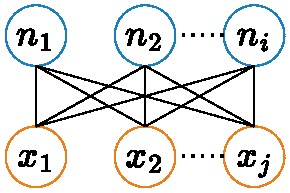
\includegraphics[width=0.6\linewidth]{figs/graph_revised.pdf}
%\caption{\small This global graph represents the environment state for $i$ agents and $j$ tasks.
%Edges encode agents ability to act on tasks.}
%\label{fig:global_graph}
%\end{figure}

%\begin{equation}
%\label{eq:node-embedding}
%\mathbf{h}_0^t = \text{Concat}\left [\text{MLP}_{\mathcal{N}}\left ( \mathcal{N}^t \right ), \text{MLP}_\mathcal{X}\left(\mathcal{X}^t \right ) \right %]\quad \mathbf{h}^t_0\in\mathbb{R}^{|\mathcal{G}^t| f_h},
%\end{equation}
We build a critic network using a GCN \cite{kipf2016semi} to propagate information between agent and task nodes by message passing. First, we use MLP encoders to map $\mathcal{N}^t$ and $\mathcal{X}^t$ into a shared latent space and concatenate them to form $\mathbf{h}_0^t$ (Alg.~\ref{alg:plato}, line~18), where $\mathbf{h}_0^t$  is the embedding of all nodes in $\mathcal{G}^t$ and $f_h$ is the hidden dimension. We then perform message passing (Alg.~\ref{alg:plato}, line~19) with a skip connection \cite{he2016deep} that adds $\mathbf{h}_0^t$ to the final layer output before pooling, preserving individual node features that would otherwise be smoothed out by message passing. We use two layers to allow information to propagate between agents and tasks through the bipartite graph.
Finally, we map the node embeddings to a scalar value by mean pooling over nodes followed by an $\mathrm{MLP}_v$ value head (Alg.~\ref{alg:plato}, lines~\ref{line:critic_pool}--\ref{line:critic_value}).
%\begin{equation}
%    \label{eq:message-passing}
%    \mathbf{h}_1 = \mathrm{ReLU}\left (\frac{\mathbf{h}_0 W_{l}}{\sqrt{|N| \cdot |X|}} \right ) + \mathbf{h}_0,
%\end{equation}


%\begin{equation}
%\label{eq:value-pooling}
%V(\text{State}^t) = MLP_v\left ( \frac{1}{|\mathcal{X}|+|\mathcal{N}|} \sum_{i=1}^{|\mathcal{X}|+|\mathcal{N}|} h^t_{2,i} \right ).
%\end{equation}

\begin{algorithm}[t]
\caption{\textsc{PLATO: Pointer Actor, GNN Critic and training}}
\label{alg:plato}
\small
\begin{algorithmic}[1]
\State \textbf{Inputs:} env $e$, horizon $T$, actor $\pi_\theta$, critic $V_\phi$, initial observation $O^0$
\For{$t=1\ldots T$} 
  \State $a^t_i\sim \textsc{PointerActor}(O_i^t) \quad \forall i \in N^t$
  \State $O^t,\text{State}^t,r^t\gets e(a^t)$
  \State $\hat V^t \gets \textsc{GNNCritic}(\text{State}^t;\phi)$;\; store $(\cdot)$
  \State  compute GAE $\hat A^t$;\; update $\theta$ by PPO-clip;\; update $\phi$ by MSE$(\hat V^t,\hat R^t)$
\EndFor
%\Statex
\Procedure{\textsc{PointerActor}}{$O_i^t$}
  \State $o_N^t,o_X^t\gets \textsc{Preprocessor}(O_i^t)$ 
  
  \State $d^t\!\gets\![\mu,\sigma^2,\min,\max](o^t_{N})$
  %\Comment{Agent Encoding}
  \State $q^t \gets \textsc{MLP}_s(d^t)$
  %\Comment{Task Encoding}
  \State $K^t \gets \{\mathrm{MLP}_x(o) \mid o \in o_X^t\} \cup \{\mathrm{MLP}_x(o_{\textsc{no-op}})\}$ 
  \State $u_x^t\!\gets\!\mathbf{v}^\top\tanh(\mathbf{W}_K k_x^t+\mathbf{W}_q q^t) \quad \forall k_x^t \in K^t$ 
  %\Comment{Pointer Decoding}
  \State  \textbf{return} $\mathrm{Cat}(\mathrm{softmax}([u_x^t]_{x \in X^t \cup \{\textsc{no-op}\}}))$
\EndProcedure
%\Statex
\Procedure{\textsc{GNNCritic}}{$\text{State}^t$} 
  \State form $\mathcal{G}^t=\langle\mathcal{X}^t,\mathcal{N}^t,\mathcal{E}^t\rangle$
  \State $h_0^t \gets \text{Concat}\left [\text{MLP}_{\mathcal{N}}\left ( \mathcal{N}^t \right ), \text{MLP}_\mathcal{X}\left(\mathcal{X}^t \right ) \right ]$
  \State $h^t_l \gets \textsc{GCN}(h^t_{l-1}, \mathcal{E}^t) \quad \text{for each layer }l$
  %\!\gets\!\mathrm{ReLU}(\tilde{D}}^{-\frac12}\tilde{A}}\tilde{D}}^{-\frac12}\mathrm{ReLU}(\tilde{D}}^{-\frac12}\tilde{A}}\tilde{D}}^{-\frac12}e}_gW}^{(1)})W}^{(2)})$

    \State $M^{(L)}\!\gets\!\frac{1}{|\mathcal{N}^t|+|\mathcal{X}^t|}\sum_i(h^t_L + h^t_0)_i$;\; \label{line:critic_pool}
  \State \textbf{return} $V=W_v\,\mathrm{MLP}_v(M^{(L)})+b_v$ \label{line:critic_value}

\EndProcedure

\end{algorithmic}
\end{algorithm}


\iffalse
In CTDE approaches, the critic processes the global state either as a single observation or as a concatenation of agent observations. This assumes a fixed number of agents and tasks, which is incompatible with openness where these sets vary over time. Padding to an upper bound is a possible workaround, but it imposes artificial constraints and defeats the purpose of handling unbounded, variable-sized systems. By instead representing the state as a bipartite graph and applying GNN layers with permutation-invariant pooling, our critic naturally accommodates changing numbers of agents and tasks while preserving relational structure, yielding a flexible and scalable value function.


\subsubsection{\textbf{Global Graph}}\label{global_graph}
This state representation allows our critic to operate on dynamic $N$ and $X$ sets. We represent the global state as a bipartite agent–task graph.
%, as in Figure ~\ref{fig:global_graph}. 
%Nodes are created first (agents, then tasks), and edges are added afterward to connect all agents to all tasks.
 This graph preserves the distinction between agents and tasks while enabling relational reasoning under dynamic, variable-sized configurations. We adopt a bipartite formulation because agents and tasks possess fundamentally different feature spaces and semantic roles. Treating them as a single homogeneous node set would conflate these differences and weaken relational reasoning. By explicitly distinguishing agents from tasks, the critic maintains their identities while still allowing full interaction modeling through graph edges, which is essential for handling openness where both sets vary in size and composition over time.  

At each timestep $t$, the global state $\text{State}^t$ is transformed into a bipartite graph $\mathcal{N}^t \in \mathbb{R}^{|N^t|\times f_N}$, where  
\begin{itemize}
\item $\mathcal{X}^t \in \mathbb{R}^{|X^t|\times f_X}$ are \emph{task nodes} and contain $f_X$ many features, describing each task at time $t$.
\item $\mathcal{N}^t \in \mathbb{R}^{|N^t|\times f_N}$ are \emph{agent nodes} and contain $f_N$ many features, describing each agent at time $t$. 
%\item $\mathcal{V} = \mathcal{A} \cup \mathcal{T}$ contains agent nodes and task nodes,  
\item $\mathcal{E}$ includes fully connected edges among all  agent-task pairs, $\{\langle n,x\rangle | n\in \mathcal{N} \text{ and }x\in \mathcal{X}\}$.  
%\item $\mathbf{X} \in \mathbb{R}^{|\mathcal{V}| \times d_x}$ holds the initial node features derived from agent observations and task attributes.  
\end{itemize}


This construction produces the global graph $\mathcal{G}^t$, which serves as the input to the MLP encoder in the next stage.
Agent nodes $\mathcal{N}$ and task nodes $\mathcal{X}$ are each projected into a shared latent dimension of size $\max(f_X, f_N)$ through learned encoders. Our bipartite edges distinguish agent relationships from task relationships, ensuring that their distinctive features are preserved while still allowing flexible relational reasoning under dynamic and unknown configurations.
%$\mathcal{X}$ and $\mathcal{N}$ are padded with a constant to $\max(f_X, f_N)$.


\subsubsection{\textbf{Node Encoder}}\label{node_encoder}
This component applies MLPs to agent and task node features of the global graph $\mathcal{G}^t$. We use this embedding as a shared latent space of heterogeneous agent and task observations.
%that heterogeneous features are projected into comparable representations for subsequent relational reasoning.
The encoder outputs the initial graph 
embedding matrix,
\begin{equation}
\mathbf{e}_g = \text{Concat}[\text{MLP}_{n}\left ( \mathcal{N} \right ), \text{MLP}_x\left(\mathcal{X} \right )]\quad e_g\in\mathbb{R}^{|\mathcal{G}^t| h}
\end{equation}
where $h$ is the hidden dimension and each row of $\mathbf{e}_g$ corresponds 
to the embedding of a node in $\mathcal{G}^t$.



\subsubsection{\textbf{Graph Convolutional Layers}}\label{gcn}
This component propagates relational information across the bipartite agent–task graph using graph convolutional layers (GCNs) \cite{kipf2016semi}, enabling each node to update its representation based on both local features and the structure of its neighbors. By aggregating information over edges, the critic captures higher-order dependencies among agents and tasks that cannot be expressed by independent node encodings alone. We use two GCN layers, first GCN layer propagates information from agents to tasks via the bipartite edges, and the second propagates back from tasks to agents, enabling indirect agent–agent interaction through two paths ($A\!\to\!T\!\to\!A$) without explicit agent–agent edges. 

\begin{equation} \label{eq:gcn}
\mathbf{H}^{(\ell)} = \text{ReLU}\!\left(\tilde{\mathbf{D}}^{-1/2} \tilde{\mathbf{A}} \tilde{\mathbf{D}}^{-1/2} \mathbf{H}^{(\ell-1)} \mathbf{W}^{(\ell)} \right),
\end{equation}
\noindent where \(\mathbf{H}^{(\ell)}\) is the node-embedding matrix at layer \(\ell\);
\(\mathbf{H}^{(0)}=\mathbf{e}_g\) is the initial node embedding;
\(\tilde{\mathbf{A}}=\mathbf{A}+\mathbf{I}\) is the adjacency with self-loops;
\(\tilde{\mathbf{D}}\) is the degree matrix of \(\tilde{\mathbf{A}}\);
\(\mathbf{W}^{(\ell)}\) is the learnable weight at layer \(\ell\);
and \(\mathrm{ReLU}(\cdot)\) is the elementwise rectifier.
We add a residual connection after the final layer to preserve local features:
\begin{equation}
\mathbf{H}^{(L)} = \mathbf{H}^{(L)} + \mathbf{e}_g.
\end{equation}



\subsubsection{\textbf{Global Pooling and Value Head}} \label{critic_valuehead}
This component aggregates the node embeddings into a fixed-size representation using permutation-invariant mean pooling, ensuring scalability to variable-sized graphs, and then maps this summary through an MLP and a linear head to estimate the centralized state value. By pooling across nodes, the critic preserves global relational information while remaining agnostic to the number and ordering of agents or tasks. This pooling operation is computed as:
\begin{equation}
\mathbf{M}^{(L)} = \frac{1}{|\mathcal{V}|} \sum_{i=1}^{|\mathcal{V}|} \mathbf{H}^{(L)}_i.
\end{equation}
\noindent\textit{where} \(\mathbf{M}^{(L)}\) is the pooled graph representation;
\(\mathbf{H}^{(L)}_i\) is the embedding of node \(i\) from the final GCN layer;
and \(|\mathcal{V}|\) is the total number of nodes (agents and tasks). This pooled vector is then mapped through a MLP to produce estimate state value, $V(\text{State}^t$:
\begin{equation}
\mathbf{V(\text{State}^t}) = \text{MLP}(\mathbf{M}^{(L)}),
\end{equation}
\noindent where \(V(\text{State}^t)\) is the centralized state value estimate at time \(t\);
and \(\mathrm{MLP}(\cdot)\) maps the pooled embedding to a scalar value through a small feedforward network.

\fi

%\paragraph{Activation Functions}
%PLATO uses standard point wise nonlinearities.
%The agent and task encoders use $\mathrm{ReLU}$ \cite{relu_agarap2018deep}, the additive-attention compatibility function uses $\tanh$, and the critic GCN layers use $\mathrm{LeakyReLU}$ \cite{leakyrelu_maas2013rectifier}.



%Mentioned in experiments generalizability section. We may add a much reduced form of this, i.e. move the theoretical comment here, but It need not mention each prop. only the overall theorem proving PLATO is well defined.
% \subsection{Generalizability}\label{sec:generalizability}

% PLATO is structurally well-defined for any number of agents and tasks, without hardcoded count bounds, padding, or configuration changes. We establish this in four propositions following a logical ordering: actor feasibility (Proposition~\ref{prop:welldefined}), ordering invariance under AO (Proposition~\ref{prop:ao}), absence of count-indexed parameters (Proposition~\ref{prop:nobound}), and critic feasibility (Proposition~\ref{prop:critic}). Full permutation-invariance derivations are in Appendix~A.7.



% \paragraph{Scope and limitations.}
% The propositions above establish \emph{structural} generalizability: the computations are always well-formed. They make no claim about \emph{statistical} generalizability — the quality of $\pi_\theta$ and $V_\phi$ on counts far outside the training distribution. A model trained on small systems may still produce unreliable outputs at large scale, even though the forward pass is numerically valid; whether learned representations transfer is an empirical question. A related computational constraint is that the GNN operates on a fully-connected bipartite graph with $|\mathcal{E}^t| = |N^t||X^t|$ edges, scaling as $O(|N^t||X^t|)$ per timestep. At very large scales — say, $|N^t| = |X^t| = 500$, yielding $2.5 \times 10^5$ edges per timestep — this quadratic growth becomes a practical bottleneck; sparse graph approximations could mitigate it but are beyond the scope of the present work. Finally, both the actor and critic assume fixed feature dimensions $f_N$ and $f_X$: if the observation space changes, retraining is required.

\subsection{Training and Complexity}\label{training}

\paragraph{Training.} 

We train PLATO under CTDE using MAPPO \cite{mappo,ppo} with a centralized critic and a single shared policy, while at execution time only the decentralized pointer actor is used. The actor is optimized with the PPO clipped objective \cite{ppo}. The critic uses the standard PPO clipped value regression loss, and we compute advantages with generalized advantage estimation (GAE) \cite{ppo,mappo,gae} (Alg.~\ref{alg:plato}, line 6). All neural components are differentiable in $\theta$ and $\phi$. The preprocessor and team statistics are deterministic tensor operations. Discrete action sampling is handled by the policy-gradient objective and is not differentiated through.  Additional details, including the network architecture and tuned hyperparameters during training, are provided in Appendix A.6. 

%\paragraph{End-to-end differentiability.} 



\paragraph{Computational complexity.}
We treat all fixed hyperparameters ($f_N$, $f_X$, $f_h$, number of GCN layers) as constants and express complexity solely in terms of the quantities that vary under openness: the number of active agents $|N^t|$ and active tasks $|X^t|$.

\paragraph{Actor.}
The preprocessor and team statistics scan $o_N^t$ and $o_X^t$ in $O(|N^t|+|X^t|)$.
The team-statistics step outputs a \emph{fixed}-length descriptor $d^t \in \mathbb{R}^{4f_N}$ regardless of $|N^t|$, so $\mathrm{MLP}_s$ contributes an $O(1)$ constant.
$\mathrm{MLP}_x$ is applied independently to each of the $|X^t|+1$ task features, costing $O(|X^t|)$; because tasks are encoded without shared state, this step parallelizes fully over the task dimension.
One-step additive attention \cite{bahdanau2014neural,ptr} computes a scalar score per key in $O(1)$ and runs over all keys in $O(|X^t|)$; \textsc{Softmax} normalization is likewise $O(|X^t|)$.
The per-agent actor cost is $O(|N^t|+|X^t|)$, and for all $|N^t|$ agents sharing the same policy the per-timestep actor cost is $O(|N^t|(|N^t|+|X^t|))$.

\paragraph{Critic.}
Node encoding via separate MLPs costs $O(|N^t|+|X^t|)$.
The bipartite graph $\mathcal{G}^t$ has $|\mathcal{E}^t|=|N^t||X^t|$ edges; each GCN layer \cite{kipf2016semi} aggregates over $|\mathcal{E}^t|$ edges in $O(|N^t||X^t|)$, which dominates the per-node projection $O(|N^t|+|X^t|)$.
With $L=2$ layers and a residual connection \cite{he2016deep}, total propagation is $O(|N^t||X^t|)$.
Mean pooling and the value head are $O(|N^t|+|X^t|)$ and $O(1)$, respectively.
The critic cost per timestep is therefore $O(|N^t||X^t|)$, which dominates the actor during training.
At execution time the critic is absent, and the cost across all agents reduces to $O(|N^t|(|N^t|+|X^t|))$ per timestep.
Since neither $|N^t|$ nor $|X^t|$ is bounded a priori, PLATO scales continuously to open environments without architectural change.



%\paragraph{End-to-end differentiability.} 



%\paragraph{Computational complexity.}
%For agent $i$, the actor costs $O(|N_i^t|+|X_i^t|)$ for preprocessing and encoders, and $O(|X_i^t|)$ for attention and softmax. The critic builds a graph with $|N^t|+|X^t|$ nodes and $|\mathcal{E}^t|$ edges; %each GCN layer costs $O(|\mathcal{E}^t| f_h)$, and pooling is $O((|N^t|+|X^t|)f_h)$.



%\paragraph{Activation functions.} %went to appendix in network architecture 
%T%he actor and critic use pointwise nonlinearities. We use $\mathrm{ReLU}$ in the MLP encoders, $\tanh$ \cite{relu_agarap2018deep} in the %additive-attention compatibility function, and $\mathrm{LeakyReLU}$\cite{leakyrelu_maas2013rectifier} in the GCN layers.



%\paragraph{End-to-End Differentiability}
%PLATO is fully differentiable with respect to all learnable neural network parameters.
%The agent encoder, task encoder, key integrator, pointer attention module, and decoder consist of affine transformations and standard nonlinear activations.
%The critic network, including node encoders, graph convolution layers, pooling, and value head, is differentiable given the constructed graph input.
%Statistical agent summaries (mean, variance, min, max) are deterministic tensor operations implemented within the neural computation graph.
%Discrete action selection is not part of the learning computation; policy optimization is performed through the differentiable log-likelihood objective.

%\paragraph{Computational Complexity}

%At each timestep, the pointer actor operates on the current agent set \(N^t\) and task set \(X^t\). The preprocessor and agent statistics computation scale linearly as \(O(|N^t|)\), while task encoding scales as \(O(|%X^t|)\). The pointer decoder applies additive cross-attention between the agent query and all task keys, yielding \(O(|X^t|)\) time and space complexity per agent. During training, the centralized critic constructs a bipartite agent--task graph with \(|N^t|+|X^t|\) nodes and \(|N^t||X^t|\) edges; each GCN layer therefore scales as \(O(|N^t||X^t|)\). With a fixed number of GCN layers and constant hidden dimensions, the overall per-timestep training complexity is dominated by the critic, while execution-time complexity remains linear in the number of available tasks.

\section{Investigations and Evaluation}\label{sec:experiments}
We evaluate PLATO on a Wildfire domain against three smart baselines and four naive heuristic-based baselines under different TO and AO configurations. We first define the configurations and summarize the methods, metrics, and training and evaluation protocols (Section~\ref{sub:experiments}). We then report our investigations on  $3\times 3$ grids under setups S0--S3: performance  (Section~\ref{sub:performance}), efficiency (Section~\ref{sub:efficiency}), and generalizability via zero-shot evaluation on an unseen $4\times 4$ grid (Section~\ref{sub:generalizability}). Domain illustrations, additional $2\times 3$ and $4\times 4$ in-domain results for all reported metrics, and zero-shot results for additional grid combinations are provided in Appendix A.1 and A.9 respectively.

%$2\times 3$ and

% =========================================
% 5.1 Experiments
% =========================================
\subsection{Experiments}\label{sub:experiments}
%(see Section~\ref{subsec:wildfire})
\paragraph{Domain.}\label{sec:to_ao_settings}  
We use the \textsc{Wildfire} domain \cite{patino2025inaugural}. A grid size $r\times c$ denotes $r$ rows and $c$ columns, for a total of $rc$ cells.
Agents are assigned to cells (no movement), and each fire (task) is associated with a cell.
Increasing the grid size expands the task location set and alters which fires fall within each agent's suppression range, thereby changing the coordination demands. Each agent carries a finite amount of \emph{suppressant}, which is consumed when suppressing fires. When depleted, the agent exits and re-enters with a stochastic \emph{refill success probability}, inducing AO. Fires have discrete \emph{sizes}; larger fires require more agents and suppression and incur larger burnout penalties if they reach terminal intensity. 
\emph{Endogenous TO } is induced by fire \emph{spread}, where existing fires probabilistically ignite neighboring cells, while \emph{exogenous TO} is induced by \emph{random ignitions} that introduce new fires independently of tasks or agents.
At each step, agents may suppress an in-range fire or select \textsc{no-op}.
Rewards are additive over time and balance positive rewards for \emph{putouts} (fires extinguished) against penalties for \emph{burnouts} (fires reaching terminal intensity).
In our experiments, we use a base reward $b=2$: putting out a fire with size $s$ yields $2^{s}$, while a burnout  yields $-2^{s}$.


\paragraph{Openness setups (S0--S3).}



Table~\ref{tab:setup_summary} summarizes our  openness setups, with increasing challenges from S0 to S3.  
S0 is closed: no new fires appear, agents have unlimited suppressant, and each episode ends once all its fires are extinguished.
S1 enables fire spread (endogenous TO) with refill success $=1$.
S2 adds random ignitions (exogenous TO) with refill success $<1$.
S3 combines spread and ignitions with AO via lower refill success. 
Setup figures are in Appendix A.2. Within a fixed 100-step horizon, openness events occur frequently in S1--S3 across all grid sizes: agents often deplete suppressant and temporarily exit (AO), and new fires appear due to spread and/or random ignitions (TO), with substantially higher counts than S0. The event frequencies by setup and grid, along with per-grid configuration parameters, contributing to different degrees of AO and TO, are reported in Appendix A.3. For complete details on the different configuration parameters across grid sizes, see Appendix A.4.


\begin{table} [h]
\centering
\footnotesize
\setlength{\tabcolsep}{3pt}
\renewcommand{\arraystretch}{1.05}

\begin{tabular}{lccc}
\toprule
\textbf{Setup} & \textbf{Fire spread} & \textbf{Random ignitions} & \textbf{Refill success} \\
\midrule
S0 & $\times$ (0.0) & $\times$ (0.0) & - \\
S1 & $\checkmark$ (0.6) & $\times$ (0.0) & 1.0 \\
S2 & $\times$ (0.0) & $\checkmark$ (0.6) & 0.8 \\
S3 & $\checkmark$ (0.6) & $\checkmark$ (0.6) & 0.6 \\
\bottomrule
\end{tabular}
\caption{Configuration: Openness mechanisms across setups. Endogenous TO is fire spread, exogenous TO is random ignitions, and AO is stochastic refill success. Numbers indicate the probability per step. Note that in S0 agents have unlimited suppressant}
\label{tab:setup_summary}
\end{table}




\paragraph{Models and baselines.}\label{sec:models_metrics} 
Our method is \textbf{PLATO}, defined as the shared pointer-network actor with an MLP encoder-decoder architecture and additive attention. We use three smart baselines that are strong approaches for coordination under partial forms of openness: \textbf{DGN}~\cite{dgn} and \textbf{DICG}~\cite{dicg} represent state-of-the-art MARL methods for dynamic coordination but assume a fixed set of agents and tasks during training; and \textbf{MOHITO}~\cite{anilmohito} is the closest prior method explicitly designed for TO.  We also use four naive baselines to contextualize gains from coordination versus simple rule-based behavior: \textbf{NOOP} always selects no-action, providing a lower bound; \textbf{Random} samples uniformly from available actions; \textbf{Strongest} prioritizes the highest-intensity fires, representing an urgency-driven heuristic; and \textbf{Weakest} prioritizes the lowest-intensity fires, reflecting an immediacy-driven strategy.

\paragraph{Metrics.} 
We evaluate policies performance using \textbf{episode return (execution average reward per episode)} and policies efficiency using \textbf{reward per fight action}. In training and evaluation, we seed each episode randomly.  Also, tables report mean $\pm$ std over 150 evaluation episodes (50 seeds per checkpoint, 3 checkpoints per method) per setup on each configuration. Bold entries are statistically significant under a one-sided paired $t$-test~\cite{student1908probable} with Bonferroni correction~\cite{hochberg1987multiple} ($\alpha{=}0.05/k$, $k$ models per table); bold cells also report the minimum Cohen's $d_z$~\cite{cohen1988statistical} effect size over all competitors. Full derivations and family definitions ($k{=}8$ main $2{\times}3$/$3{\times}3$, $k{=}4$ main $4{\times}4$ and zero-shot, $k{=}6$ ablation) are in Appendix~\ref{sec:convergence_appendix}. Training, validation, and evaluation seeds are drawn from disjoint ranges; see Appendix~\ref{app:random_seed} for details.

%We therefore report results aggregated over many independent evaluation episodes and apply the same checkpoint-selection procedure to all methods.  



\subsection{Performance}\label{sub:performance}
As shown in Table 2, under openness, PLATO achieves the highest return in S2 and S3 with statistical significance, while remaining comparable to the top-performing baselines in S1. In S0 with no openness, PLATO performs as well as all top-performing baselines. MOHITO now converges competitively in S3 but still lags in S1--S2.


%Under openness, PLATO matches the best return in S1 and achieves the highest return in S2 with statistical significance (Table~\ref{tab:reward_3x3}). In S3, DGN achieves the highest return. Overall, PLATO is strongest in S2 and remains competitive in S1--S3 relative to the other methods. 
%In the closed setup (S0), the best naive baselines match the best smart baselines, consistent with the fixed initial fires being fully extinguishable by simple heuristics. See Appendix A.9 for more detailed discussions.

%As expected because S1--S3 induce frequent ignitions and zero-suppressant exits, so many suppression actions are low-value unless they can finish a putout before a costly $-2^{s}$ burnout; PLATO’s higher reward per fight action in S1--S3 (Table~\ref{tab:rpf_3x3}) indicates more selective, higher-yield suppression. In contrast, the smart baselines show low or negative reward per fight action under openness (e.g., MOHITO drops to $-0.74$ in $3\times 3$ S3), consistent with less coordinated (or most wasteful) suppression effots and burnout-driven return collapse when TO and AO are combined.
% -----------------------
% Reward (3x3 only, main) [UPDATED]
% -----------------------
\begin{table}[t]
\centering
\small
\setlength{\tabcolsep}{2.5pt}
\renewcommand{\arraystretch}{1.03}
\begin{tabular}{l|l|l|l|l}
\toprule
\multicolumn{5}{c}{$3\times 3$} \\
\midrule
Model & \multicolumn{1}{c|}{S0} & \multicolumn{1}{c|}{S1} & \multicolumn{1}{c|}{S2} & \multicolumn{1}{c}{S3} \\
\midrule
PLATO & 8.00$\pm$0.00 & 7.68$\pm$1.36 & \textbf{115.44$\pm$10.82} & \textbf{81.76$\pm$19.20} \\
DICG & 8.00$\pm$0.00 & 6.00$\pm$2.71 & 61.44$\pm$13.41 & 42.72$\pm$16.94 \\
DGN & 7.76$\pm$0.96 & 5.60$\pm$2.68 & 45.08$\pm$16.07 & 32.88$\pm$15.21 \\
MOHITO & 8.00$\pm$0.00 & 4.32$\pm$3.01 & 48.32$\pm$20.18 & 51.40$\pm$16.99 \\
NOOP & -8.00$\pm$0.00 & -8.00$\pm$0.00 & -12.00$\pm$0.00 & -12.00$\pm$0.00 \\
Random & 6.00$\pm$2.46 & 4.48$\pm$3.49 & 11.48$\pm$16.06 & 0.88$\pm$12.96 \\
Weakest & 8.00$\pm$0.00 & 7.76$\pm$0.96 & 70.36$\pm$22.66 & 37.44$\pm$1.72 \\
Strongest & 8.00$\pm$0.00 & 7.28$\pm$1.75 & 24.24$\pm$29.13 & 13.92$\pm$20.38 \\

\bottomrule
\end{tabular}
\caption{Performance: Episode return (mean $\pm$ std) on the $3\times 3$ grid. Bold indicates statistically significant best performance within each setup (one-sided paired $t$-test; $\alpha=0.00625$).}
\label{tab:reward_3x3}
\end{table}




% =========================================
% 5.3 Efficiency
% =========================================
As shown in Table~\ref{tab:rpf_3x3}, PLATO attains the highest reward per fight (i.e., efficiency) with statistical significance in S0, S2, and S3, whereas S1 is led by the \textbf{Weakest} heuristic. Across methods, reward per fight is generally lower under higher openness (S2, S3) than in S0/S1, and PLATO remains positive across S0--S3 in its efficiency.
%We further analyze efficiency using reward per fight action (Table~\ref{tab:rpf_3x3}), i.e., reward obtained per suppression attempt. Across setups, PLATO attains the highest reward per fight in S1 and S2 with statistical significance. In S3, reward per fight is similar among the top methods (DGN/DICG/PLATO). For most methods, reward per fight is lower in S2/S3 than in S0/S1. PLATO remains positive across S0--S3. More supporting results are in Appendix A.9. Note also that reward per fight action generally decreases under higher openness (S2, S3) as suppressant scarcity and coordination demands increase. 
%PLATO's ability to maintain a positive reward per fight action also shows its robustness in handling openness.  
% -----------------------
% Reward per Fight (3x3 only, main) [UPDATED]
% -----------------------
\begin{table}[t]
\centering
\small
\setlength{\tabcolsep}{2.5pt}
\renewcommand{\arraystretch}{1.03}
\begin{tabular}{l|l|l|l|l}
\toprule
\multicolumn{5}{c}{Reward per Fight ($3\times 3$)} \\
\midrule
Model & \multicolumn{1}{c|}{S0} & \multicolumn{1}{c|}{S1} & \multicolumn{1}{c|}{S2} & \multicolumn{1}{c}{S3} \\
\midrule

PLATO & \textbf{1.30$\pm$0.23} & 0.55$\pm$0.39 & \textbf{0.77$\pm$0.07} & \textbf{0.65$\pm$0.09} \\
DICG & 0.48$\pm$0.35 & 0.33$\pm$0.21 & 0.47$\pm$0.08 & 0.39$\pm$0.16 \\
DGN & 0.69$\pm$0.39 & 0.50$\pm$0.48 & 0.39$\pm$0.10 & 0.33$\pm$0.14 \\
MOHITO & 0.89$\pm$0.00 & 0.34$\pm$0.37 & 0.34$\pm$0.32 & 0.42$\pm$0.12 \\
NOOP & -8.00$\pm$0.00 & -8.00$\pm$0.00 & -12.00$\pm$0.00 & -12.00$\pm$0.00 \\
Random & 0.73$\pm$0.36 & 0.38$\pm$0.39 & 0.03$\pm$0.49 & -0.22$\pm$0.47 \\
Weakest & 1.03$\pm$0.13 & \textbf{0.87$\pm$0.44} & 0.48$\pm$0.07 & 0.35$\pm$0.02 \\
Strongest & 1.03$\pm$0.13 & 0.71$\pm$0.57 & -0.10$\pm$0.62 & -0.16$\pm$0.57 \\

\bottomrule
\end{tabular}
\caption{Efficiency: Reward per fight (mean $\pm$ std) on the $3\times 3$ grid. Bold indicates statistically significant best performance within each setup (one-sided paired $t$-test; $\alpha=0.00625$).}
\label{tab:rpf_3x3}
\end{table}




% =========================================
% 5.4 Generalizability
% =========================================
\subsection{Generalizability}\label{sub:generalizability}
Robustness to the nonstationary environment is the most important challenge in openness as just one more agent or task may appear which changes the optimal strategy. Theoretically, we show in, Thm. \ref{theorem:well-defined}, that PLATO's actor and critic are well defined functions over an unbounded state space. Empirically, we evaluate generalization by executing policies trained on $3\times 3$ directly on an unseen $4\times 4$ grid without further training. Table~\ref{tab:cross_4x4_reward_3x3} shows that PLATO and DICG generalize effectively to the unseen grid, while DGN and MOHITO degrade under zero-shot conditions in S1. No method achieves statistical significance in S2--S3; DICG leads S2 and PLATO leads S3 numerically. DGN drops near-zero in S1 and MOHITO turns negative in S1, consistent with sensitivity to changes in agent and task composition, while both recover partially in S2--S3.
%DICG remains competitive but below PLATO across open setups.
%on $2\times 3$ or
%We evaluate generalization by executing policies trained on $3\times 3$ directly on an unseen $4\times 4$ grid without further training. Whereas PLATO supports variable agent and task sets by design, we adapt the other three smart baselines to varying numbers of agents and tasks: DGN and DICG are padded to 30 agents and 30 tasks; MOHITO handles task openness natively but assigns agent-specific policies, so unseen agents receive a randomly sampled trained policy. Across setups, all smart baselines exhibit different zero-shot behavior. PLATO is competitive across S0--S3 and attains the highest mean return in S3 (Table~\ref{tab:cross_4x4_reward_3x3}). Relative to PLATO, DGN degrades substantially in S2 and is negative in S3, while MOHITO and DICG remain strong in S1/S2 but drop in S3. Additional supporting results are in Appendix A.9. %DGN is consistently outperformed (negative in S1--S3 for both training grids); DICG is less stable (e.g., $2\times 3$-trained collapses to $-4.00$ in S3); across all four setups, MOHITO performs relatively similarly with PLATO outperfoming MOHITO in S3. %Under combined openness (S3), all methods suffer with negative rewards. 

 %Note that training grid sizes affect the zero-shot performance as expected, e.g., PLATO trained on $2\times 3$ degrades under openness, while PLATO trained on $3\times 3$ transfers more effectively.
 
%PLATO's pointer actor performs content-based, slot-free selection over the currently available fires conditioned on the current agent set, reducing train-test mismatch when the $4\times 4$ grid changes each agent’s in-range task set. In contrast, padding-based fixed-slot models (i.e., DGN and DICG) and agent-specific policies (i.e., MOHITO) are more sensitive to changes in task composition and agent availability, increasing wasted suppression (see more results in Appendix A.9).
% -----------------------
% 4x4: Reward (zero-shot), trained on 3x3 (main)
% -----------------------

\begin{table}[t]
\centering
\footnotesize
\setlength{\tabcolsep}{3.2pt}
\renewcommand{\arraystretch}{1.03}
\begin{tabular}{@{}l|c|c|c|c@{}}
\toprule
\multicolumn{5}{c}{Trained on $3\times 3$; tested on $4\times 4$} \\
\midrule
Model  & \multicolumn{1}{c|}{S0} & \multicolumn{1}{c|}{S1} & \multicolumn{1}{c|}{S2} & \multicolumn{1}{c}{S3} \\
\midrule

PLATO & 10.00$\pm$2.68 & 5.40$\pm$8.36 & 58.24$\pm$19.84 & 57.72$\pm$17.63 \\
DICG & 10.40$\pm$1.67 & 8.56$\pm$8.50 & 63.28$\pm$11.83 & 51.60$\pm$14.19 \\
DGN & 6.96$\pm$4.00 & -0.44$\pm$6.34 & 49.52$\pm$19.37 & 37.48$\pm$27.22 \\
MOHITO  & \textbf{11.28$\pm$1.88} & -1.28$\pm$7.56 & 42.84$\pm$28.12 & 56.56$\pm$9.85 \\

\bottomrule
\end{tabular}
\caption{Generalizability: Episode return on $4\times 4$ under zero-shot evaluation 
when trained on $3\times 3$ (mean $\pm$ std). Bold indicates statistically significant 
best performance within each setup (one-sided paired $t$-test; $\alpha=0.0125$).}
\label{tab:cross_4x4_reward_3x3}
\end{table}

\subsection{Summary}\label{sub:exp_summary}
Overall, the results show three main trends. First, PLATO achieves the highest performance in S2 and S3 on the $3\times 3$ grid with statistical significance. Second, PLATO achieves the highest efficiency in S0, S2, and S3, while remaining positive across all setups. Third, under zero-shot transfer to $4\times 4$, PLATO and DICG generalize effectively while DGN and MOHITO collapse in S1; PLATO leads S3 and DICG leads S2 numerically. Additional results are in Appendix~A.9.

%significant separation across methods.

\section{Ablation}\label{sec:ablation}

We ablate four PLATO design choices: the actor encoder-decoder (MLP~\cite{rumelhart1986learning_mlp} vs.\ LSTM~\cite{lstm}), the pointer scoring function (additive attention~\cite{bahdanau2014neural} vs.\ dot-product), team statistics, and the GNN critic. Table~\ref{tab:ablate_reward_stacked_3x3_4x4} shows the results (details in Appendix~A.10). No-TS and No-GNN denote MLP+additive variants with team statistics or the GNN critic removed, respectively.

%The goal is to test whether temporal memory improves performance as task and agent sets vary, and how learned compatibility in the scorer beyond similarity-based pointing impacts the performance, respectively. All variants share the same critic, training objective, and hyperparameters, isolating the effect of each component. LSTM-based implementations use temporal memory while MLP-based ones do not. Additive-based implementations use learned compatibility in the scorer while dot-product-based ones use similarity in the projected embedding space. 






% -----------------------
% Ablations: Reward (3x3) + 4x4 Reward (zero-shot, trained on 3x3)
% -----------------------
\begin{table}
\centering
\small
\setlength{\tabcolsep}{2.2pt}
\renewcommand{\arraystretch}{1.02}

% -------- 3x3 --------
\begin{tabular}{@{\hspace{2pt}}l|l|l|l|l@{\hspace{2pt}}}
\toprule
\multicolumn{5}{c}{Trained and tested on $3\times 3$} \\
\midrule
Variant & \multicolumn{1}{c|}{S0} & \multicolumn{1}{c|}{S1} & \multicolumn{1}{c|}{S2} & \multicolumn{1}{c}{S3} \\
\midrule
MLP, add    & 8.00$\pm$0.00 & 7.68$\pm$1.36 & 115.44$\pm$10.82 & 81.76$\pm$19.20 \\
LSTM, add   & 8.00$\pm$0.00 & 7.60$\pm$1.21 & 118.12$\pm$10.58 & 86.56$\pm$19.23 \\
MLP, dot    & 8.00$\pm$0.00 & 7.28$\pm$1.55 & 110.96$\pm$12.55 & 87.36$\pm$17.19 \\
LSTM, dot   & 8.00$\pm$0.00 & 7.76$\pm$0.96 & 117.60$\pm$13.24 & 89.84$\pm$17.78 \\
No-TS       & 8.00$\pm$0.00 & 7.76$\pm$1.25 & 104.68$\pm$11.05 & 71.76$\pm$19.83 \\
No-GNN      & 8.00$\pm$0.00 & 7.60$\pm$1.46 & 110.84$\pm$12.87 & 82.40$\pm$21.91 \\
\bottomrule
\end{tabular}

\vspace{4pt}

% -------- train 3x3, test 4x4 --------
\begin{tabular}{@{\hspace{2pt}}l|l|l|l|l@{\hspace{2pt}}}
\toprule
\multicolumn{5}{c}{Trained on $3\times 3$; tested on $4\times 4$} \\
\midrule
Variant & \multicolumn{1}{c|}{S0} & \multicolumn{1}{c|}{S1} & \multicolumn{1}{c|}{S2} & \multicolumn{1}{c}{S3} \\
\midrule
MLP, add    & 10.00$\pm$2.68 & 5.40$\pm$8.36 & 58.24$\pm$19.84 & 57.72$\pm$17.63 \\
LSTM, add   & 10.16$\pm$3.02 & 8.24$\pm$12.19 & 42.08$\pm$25.14 & 59.68$\pm$14.72 \\
MLP, dot    & 10.32$\pm$2.11 & 4.16$\pm$5.09 & 51.84$\pm$26.84 & 63.52$\pm$15.21 \\
LSTM, dot   & 10.72$\pm$2.38 & 4.80$\pm$5.55 & 40.96$\pm$30.22 & 62.52$\pm$10.45 \\
No-TS       & 9.44$\pm$2.80 & 5.76$\pm$8.49 & 42.12$\pm$25.72 & 52.36$\pm$27.08 \\
No-GNN      & 9.60$\pm$2.83 & 6.60$\pm$11.13 & 45.52$\pm$28.72 & 49.40$\pm$25.60 \\
\bottomrule
\end{tabular}

\caption{PLATO ablations: episode return (mean $\pm$ std) on $3\times 3$ and zero-shot episode return on $4\times 4$ (mean $\pm$ std) when trained on $3\times 3$. Bold indicates statistically significant best performance within each setup (one-sided paired $t$-test; $\alpha\approx0.0083$).}
\label{tab:ablate_reward_stacked_3x3_4x4}
\end{table}


% ==========================
% ANALYSIS
% ==========================




\textbf{Does temporal memory improve task selection under openness and zero-shot?} The impact of temporal memory is marginal. On $3\times 3$, MLP+additive and LSTM+additive achieve comparable returns (S2: $115.44$ vs $118.12$; S3: $81.76$ vs $86.56$), with neither variant consistently dominating in zero-shot $4\times 4$. We adopt MLP+additive as our primary variant for its lower computational overhead with comparable performance.

\textbf{Does learned compatibility improve task selection under openness?} Additive attention provides a clear advantage under moderate openness: on $2\times 3$ S1, additive variants score $65.48$/$69.96$ versus dot-product $42.36$/$33.48$ (see Appendix~A.10). At $3\times 3$ the gap narrows (S2: $115.44$ vs $110.96$), with both scorers competitive at larger scale. The learned compatibility function via $W_q$, $W_K$, and $v$ proves more robust when task and agent sets vary, particularly at lower scales where openness is more pronounced.

\textbf{Does team context aid task selection under openness?} Removing team statistics consistently reduces performance across grids. On $2\times 3$ S1, reward falls from $65.48$ to $51.12$; on $3\times 3$ S2 from $115.44$ to $104.68$; and under zero-shot $4\times 4$ (trained on $3\times 3$) S2 from $58.24$ to $42.12$. The fixed-size aggregation (mean, variance, min, max over $N^t$) provides a reliable team context independent of agent count, which is essential under AO.

\textbf{Does a graph-structured critic improve generalization?} The GNN critic's benefit is most pronounced under zero-shot transfer. On native $3\times 3$, removing it reduces S2 reward modestly ($115.44 \to 110.84$). Under zero-shot to $4\times 4$ (trained on $3\times 3$), the degradation is larger: S2 drops $58.24 \to 45.52$ and S3 drops $57.72 \to 49.40$. The graph-structured value function captures structural team dependencies that support generalization to unseen grid scales.


%\paragraph{Q1: Does temporal memory improve task selection under openness and zero-shot?}
%Temporal memory yields selective gains. MLP+additive is stronger on $2\times 3$ across S1--S3, while on $3\times 3$ and zero-shot $4\times 4$ the LSTM variant mainly helps in the most challenging Setup 3 (combined TO and AO), consistent with memory supporting coordination when tasks and agent availability change rapidly (Tables~\ref{tab:ablate_reward_stacked_2x3_3x3}, \ref{tab:ablate_4x4_reward_stacked}).

%\paragraph{Q2: Does learned compatibility improve task selection under openness?}
%Additive attention consistently outperforms dot-product across grids and in zero-shot, while dot-product often degrades sharply under higher openness (Tables~\ref{tab:ablate_reward_stacked_2x3_3x3}, \ref{tab:ablate_4x4_reward_stacked}). This indicates that openness requires a scorer that can model task-agent compatibility, not simply embedding similarity.

%\paragraph{Implications for addressing openness.}
%We have clear evidence that additive attention is the more reliable scorer: it learns a compatibility function via $W_q$, $W_K$, and $v$, which is more robust to shifting task sets and agent availability than dot-product similarity. However, the impact of temporal memory in handling openness is less clear: an MLP encoder is sufficient for moderate openness, but an LSTM can be beneficial under combined TO and AO, especially in a zero-shot training generalization scenario.




\section{Related Work}\label{sec:related}



%In this section, we review several existing methods that address aspects of openness or dynamic adaptability in multi-agent systems, including the techniques used in our investigations:  DGN~\cite{dgn}, DICG~\cite{dicg}, and GPL~\cite{gpl}, which focus on dynamic multi-agent coordination, and MOHITO~\cite{anilmohito}, which is specifically designed for task openness. We also discuss transformer-based models and briefly review multi-task, curriculum, and dynamic single-agent reinforcement learning approaches that adapt to evolving environments.

Graph Neural Networks (GNNs) \cite{gnn} model multi-agent interactions flexibly by representing agents as graph nodes and using message-passing to aggregate neighbor information, naturally handling variable group sizes but often limiting openness by imposing bounded assumptions. Several dynamic multi-agent approaches partially address related challenges. DGN~\cite{dgn} uses graph convolution with fixed-size neighbor communication for cooperation and can generalize to larger teams but restricts interaction through a predefined neighborhood and assumes static goals. DICG~\cite{dicg} learns dynamic coordination graphs for multi-agent coordination, handling large fixed teams well but requires known agent and task sets in advance, limiting true openness. GPL~\cite{gpl} tackles AO in ad hoc teamwork with graph neural nets and type inference for variable team sizes but trains only a single agent while others have fixed policies, thus not a fully adaptive multi-agent training approach. In contrast, MOHITO~\cite{anilmohito} is specifically designed for openness, formalizing task-open Markov games and employing hypergraph-based actor–critics to handle dynamic task–action sets, though it focuses solely on TO and assumes fixed agents and frames. Our investigations show that PLATO achieves superior performance compared to DGN, DICG, and MOHITO, with clear gains in harder openness setups, demonstrating the effectiveness of PLATO's pointing mechanism as an unbounded solution.
%transformers needs citations.

Also, while some may argue that transformers \cite{vaswani2017attention} naturally handle unbounded input sizes, imposing bounds is necessary to maintain training efficiency and scalability. That is, though transformers theoretically support variable-length inputs by attending over all tokens---making them attractive to OASYS, to enable efficient parallelization, \emph{inputs are typically padded to fixed lengths}.  This practice limits transformer-based applications in OASYS to a maximum number of agents or tasks. PLATO, on the other hand, circumvents this limitation via the attention mechanism and team-based statistics to handle variability in agents and tasks.  

Related fields such as multi-task reinforcement learning~\cite{zhang2021survey} and curriculum learning~\cite{narvekar2020curriculum} focus on adapting to varying tasks or progressively harder scenarios but typically assume a fixed number of entities and do not address AO and TO.  Also, they may suffer from catastrophic forgetting when learning new tasks~\cite{ribeiro2019multitask}, high prediction errors in volatile environments, and do not effectively handle openness due to their reliance on predefined task spaces or curriculum structures~\cite{kravchenko2024limitations}. %Dynamic single-agent reinforcement learning approaches can handle changing environment characteristics but remain limited to single-agent settings, exhibit poor sample efficiency in complex scenarios, and do not consider the multi-agent coordination challenges inherent in our open systems framework where agents, tasks, and interaction patterns can change simultaneously and unboundedly.




%\subsection{Related GNN-Based Approaches}\label{related:gnn}
%Graph neural networks (GNNs)~\cite{gnn} model agent interactions through message passing on graphs, naturally supporting variable team sizes. However, most GNN-based MARL methods still impose bounded adjacency or task sets, limiting full openness.

%GNNs \cite{gnn} offer a flexible framework to model multi-agent interactions in variable-sized groups by representing agents as nodes in a graph. In a GNN-based approach, edges (or an adjacency function) define which agents interact, and message-passing or convolution operations allow each agent to aggregate information from its neighbors. This graph-based representation naturally adapts when the team composition or interaction topology changes, without requiring a fixed input size. Several prior MARL approaches have attempted to handle aspects of openness, though each has limitations. In summary, they still impose bounds or assumptions that limit true openness. 

%For example, a standard multilayer perceptron (MLP) \cite{rumelhart1986learning_mlp} or Convolutional Neural Network (CNN) \cite{lecun2002gradient_cnn} requires a fixed-size input vector, so handling a variable number of entities often means padding the input to a maximum size and using masking to ignore the dummy entries or dynamically changing action spaces. This introduces an implicit upper bound on how many entities can be handled. Similarly, transformer-based \cite{wolf2020transformers} or attention-based \cite{vaswani2017attention} models input sequences are padded to a fixed length and masked. These workarounds mean the model is only trained up to a certain capacity – scenarios with more agents, task, or new frames beyond this will fall outside its training distribution. Prior multi-agent RL methods that appear to handle dynamic teams typically rely on such fixed-size placeholders. It has been observed that a changing number of agents yields a state representation of variable length, which causes traditional RL methods with fixed-length state vectors to perform poorly. In other words, without a specially designed architecture, the model either fails to process a different team size or must be tricked via padding/masking, often degrading performance in unseen or un-bounded conditions caused by openness.

%paragraph 4 DGN:
%DGN
%Graph Convolutional Reinforcement Learning (DGN) \cite{dgn} introduced a GNN-based method for multi-agent cooperation, where each agent shares parameters and communicates with a fixed number of neighbors (e.g., k-nearest agents) through graph convolution. This technique allows DGN to generalize to scenarios with more agents than seen in training (by exploiting relation kernels and neighbor-based message passing). However, DGN still imposes a structured communication graph (with a chosen neighborhood size k), effectively bounding the interactions and not truly allowing an unbounded number of agents beyond the predefined graph connectivity. Moreover, it assumes a static task goal and does not explicitly address agents entering or leaving during an episode.


%paragraph 5 MOHITO:

%MOHITO \cite{anilmohito} is one of the few approaches in MARL that explicitly tackles TO. It formalizes this setting with task-open Markov games (TaO-MG) and represents agent–task–action relations using interaction hypergraphs, which are converted into incidence graphs and processed by graph attention networks within an actor–critic framework. This enables reasoning over dynamically changing task–action sets without relying on a fixed task universe. MOHITO demonstrates effective performance in task-open domains such as ridesharing and wildfire, but it focuses solely on TO and does not address AO or FO.
%SHOULD I talk about the scalability of MOHITO and the perfomance (unbiasadli)? TODO

%paragraph 6 DICG:

%Deep Implicit Coordination Graphs (DICG) \cite{dicg} similarly leverage a graph-structured approach: DICG learns to infer a dynamic coordination graph among agents and uses a graph neural network to approximate the joint action-value function. This enables coordination in environments with many agents by learning which agents should interact for a given situation. However, DICG \cite{dicg} still presumes a fixed set of agents and tasks during training; it excels at coordinating large teams, but not at handling new agents or tasks appearing ad hoc. Any task openness in DICG’s experiments is limited to toggling the activity of known tasks (activating or deactivating predefined objectives), rather than introducing entirely new objectives. In other words, the set of possible tasks remains fixed, representing only a low level of task openness. DICG does not support unboundedness in the problem definition, since the universe of agents and tasks must be modeled in advance.

%paragraph 7 GPL:
%Graph-based Policy Learning (GPL) \cite{gpl} addresses agent openness in ad hoc teamwork \cite{stone2010ad}, where teammates with different fixed policies may enter or leave dynamically. GPL assumes that teammate types are fixed, implemented as heuristics or pretrained policies, and focuses on training a single learning agent rather than a full multi-agent system. Although it employs graph neural networks and coordination graphs to handle variable team sizes and is in principle unbounded in the number of teammates it can model, GPL is not a multi-agent reinforcement learning approach in the strict sense, since only one agent is being trained while others remain fixed. Its architecture combines type inference, an agent model to predict teammate actions, and a joint action value model to estimate their impact on the learner’s returns, to maximize the learner's single reward in the team.



%\subsection{Transformers}\label{sec:related}

%Transformers are a class of deep neural network architectures built on multi-head self-attention mechanisms, originally introduced for sequence modeling tasks like machine translation \cite{vaswani2017attention}. In a transformer, each element of the input can attend to every other element, enabling the model to capture rich dependencies without the sequential bottleneck of recurrent networks. This attention-based design allows transformers to process all input tokens in parallel and model long-range or pairwise relationships effectively. One major advantage over recurrent sequence-to-sequence models is this parallelization, which significantly accelerates training. In principle, transformers can accept variable-length sequences since their computations scale with the number of input tokens rather than requiring a fixed input size. This flexibility makes them attractive for MARL settings with dynamic agent or task sets, as the self-attention could, in theory, adapt to changing input sizes by attending over all present entities.

%However, in practice, efficient batching on GPUs/TPUs requires inputs to share a consistent tensor shape. To achieve this, implementations typically pad or truncate sequences to a uniform length and apply masks so that attention ignores dummy tokens \cite{wolf2020transformers}. While this enables fast parallelization, it introduces an implicit upper bound on the number of tokens the model can handle, wastes computation on padded positions, and constrains scalability. For instance, popular transformer networks set a maximum sequence length to control memory usage and quadratic runtime complexity, which becomes prohibitive as the number of entities grows \cite{tay2023efficient}.

%In the context of OASYS, this means transformer-based policies still assume a maximum number of agents or tasks, limiting their ability to handle true unbounded openness. Although adaptations such as set transformers avoid padding, they often sacrifice training efficiency \cite{lee2019set}. Overall, while theoretically flexible, transformers in practice remain constrained by padding, masking, and implicit upper bounds in most MARL applications with some form of openness.

 


%\section{Limitation}\label{sec:limitation}
%\input{sections/8-limitations}


%\section{Future Works}\label{sec:future}
%\input{sections/9-future}



\section{Conclusion}\label{sec:Conclusion}
\input{sections/11-Conclusion}

\section{Acknowledgment}\label{sec:acknowledgment}
This work was supported in part by grant ANONYMIZED. We extend our special thanks to ANONYMIZED, for their invaluable feedback, discussions, and support throughout the development of this research.


%%%%%%%%%%%%%%%%%%%%%%%%%%%%%%%%%%%%%%%%%%%%%%%%%%%%%%%%%%%%
\bibliographystyle{plainnat}
\bibliography{references}

\appendix
%%%%%%%%%%%%%%%%%%%%%%%%%%%%%%%%%%%%%%%%%%%%%%%%%%%%%%%%%%%%

\section{Appendix}\label{sec:appendix}


\section{Proofs}



% \subsection{Statistics-permutation invariant proof}
% The statistics $[\mu, \sigma^2, \min, \max]$ computed over agents are permutation-invariant.
% \begin{proof}
% Let $\pi$ be any permutation of $\{1, \ldots, |N^t|\}$. For rows $\{o_1, \ldots, o_{|N^t|}\}$ of $o^t_N$:
% \begin{itemize}
%     \item $\mu = \frac{1}{|N^t|}\sum_{i} o_i = \frac{1}{|N^t|}\sum_{i} o_{\pi(i)}$ (addition is commutative)
%     \item $\sigma^2 = \frac{1}{|N^t|}\sum_{i} (o_i - \mu)^2 = \frac{1}{|N^t|}\sum_{i} (o_{\pi(i)} - \mu)^2$
%     \item $\min_i o_i = \min_i o_{\pi(i)}$ (minimum over a set is order-independent)
%     \item $\max_i o_i = \max_i o_{\pi(i)}$ (maximum over a set is order-independent)
% \end{itemize}
% Thus $d^t = [\mu, \sigma^2, \min, \max]$ is invariant to agent ordering.
% \end{proof}



\subsection{Well Defined PLATO}

A precondition to learning a rational policy in openness is producing consistent actor queries from finite parameters conditioned on a countably infinite observation space. In other words, a well defined function. GNN actors, such as MOHITO \citep{anilmohito}, meet this inherently because graph convolution is permutation invariant to node ordering and produce observation specific action output from its hyperedges. Here we prove that PLATO also fulfills this requirement.

To prove PLATO is a well defined function we will show the actor, $\pi$, and critic, $V$, have values for each state in this unbounded space,
$$
\begin{aligned}
    & (1) \forall s \in \mathbf{S}, \exists\Delta A \subseteq \mathbf{A}: (s,\Delta A) \in \pi
    \qquad (2) \forall s \in \mathbf{S} \exists v \in \mathbb{R}: (s,v) \in V,
\end{aligned}
$$
and that they consistently produce only one finite action distribution and $v$ approximation for each state,
$$
\begin{aligned}
    &(3) \forall s \in \mathbf{S}, \quad \forall \Delta A_1, \Delta A_2 \subseteq \mathbf{A}: (s,\Delta A_1), (s,\Delta A_2) \in \pi\\
    &(4) \forall s \in \mathbf{S}, \quad \forall v_1,  v_2 \in \mathbb{R}: (s,v_1), (s,v_2) \in V.
\end{aligned}
$$


% First we show that PLATO's pointer network actor stochastic policy's are well defined over the entire unbounded observation space we condition them on,

% \begin{proposition}[Actor well-definedness under openness]\label{prop:welldefined}
% For any $|N^t| \geq 1$ and $|X^t| \geq 0$, and for fixed parameters $\theta$, the PLATO actor $\pi_\theta(\cdot \mid o_i^t)$ is a well-defined categorical distribution over $|X^t|+1$ actions.
% \end{proposition}

\begin{proof}[Proof (1)]
    \label{proof:definedpi}
    Assume there exists a state, $\hat{s} \in \mathbf{S}$ where $\pi(\hat{s})\neq \Delta A \subseteq \mathbf{A}$. It must then be true that either $\pi(\hat{s})$
 is undefined, in other words $\hat{s} \notin \pi$, or $\pi(\hat{s})$ must have support over an action not in $\mathbf{A}$.
 
    PLATO's actor preprocessor factors agent observations $o_i^t \to (o_N^t, o_X^t)$ of shapes $(|N^t| \times f_N,|X_i^t|\times f_X)$.  Where $X^t_i$ here refers to tasks agent $i$ can act on; $X_i^t\subseteq X^t$. We assume this factorization is given by the environment and defined over $\Psi_\Omega$. Regarding agent observations, team statistics produce $d^t \in \mathbb{R}^{4f_N}$, a \emph{fixed}-length vector regardless of $|N^t|$. The subsequent MLP is defined over $\mathbb{R}^{4f_n}$. On the task observations, the task encoding applies individually to tasks and is thus defined over $\mathbb{R}^{f_x}$, and produces keys, $K^t \in \mathbb{R}^{(|X^t|+1)f_h}$. Each score $u_x^t = \mathbf{v}^\top\!\tanh(\mathbf{W}_K k_x^t + \mathbf{W}_q q^t)$ applies the same fixed-parameter function regardless of $|X^t_i|$ or $|N^t|$. Because the only input constraints come from $\Psi_\Omega$, and $\Psi_\Omega$  is defined over all possible task and agent sets, $s\in \pi \iff s \in \mathbf{S}$. It must be the case that $\hat{s} \in \pi$.

There exists one score $u_x^t \forall X_i^t \in M^t$ and one NO-OP score. PLATO assumes that there exists one action per task, $a_X \forall X_i$. There are also additional task-agnostic actions $A_*$, here a NO-OP action.  If the environment's action space is defined as, $\Psi_A(...) = \prod_{i}\{a_x  | x \in X_i, X_i\subseteq X\} + \{a_{NOOP}\}$, then any task score set must only include $a_x \forall X_i$ and NO-OP by definition. It must be the case that $\pi(\hat{s})\subseteq A$. Thus, by contradiction  $\forall s \in \mathbf{S}, \exists\Delta A \subseteq \mathbf{A}: (s,\Delta A) \in \pi$. 
\end{proof}


\begin{proof}[Proof (2)]
    \label{proof:definedq}
    The global graph is a partition over the state, similar to the preprocessor's output, but encompassing all agents' local observations. If the factored agent, $\mathcal{N}$  and task nodes $\mathcal{X}$, have fixed feature dimensions, $f_\mathcal{N}, f_{\mathcal{X}}$, the critic's MLPs can encode them into a shared latent space, $\mathbb{R}^{f_h}$.  The subsequent layers are GCNs over these nodes which are defined for a fixed $f_h$, global mean pooling which has no spatial requirements, and a decoder MLP, $MLP_v: \mathbb{R}^{f_h}\to \mathbb{R}$. Thus, if tasks and agents can be factored into state feature representations of fixed length regardless of change in the overall task and agent sets then,  $\forall s \in \mathbf{S} \exists v \in \mathbb{R}: (s,v) \in V$.
\end{proof}

\begin{proof}[Proof (3)]
    \label{proof:mappingpi}
        Let $\sigma(o_i^t)$ represent a permutation of task and agent observations given by the environment. The preprocessor is not assumed to be permutation invariant, in that \textbf{only the} order of factors may change by the order of input observations. The agent encoder is permutation invariant because the team statistics are comprised of permutation invariant operations, (mean, variance, minimum, maximum). The task encoder operates on all $o_x^t \in o_X^t$ independently and like the preprocessor persists ordering, but $K^t$'s values are unaffected by the order. The pointer decoder does not use a positional embedding, and more specifically,
$$
\mathbf{v}^\top\!\tanh(\mathbf{W}_K \sigma(k_x^t) + \mathbf{W}_q q^t) = \mathbf{v}^\top\!\tanh(\mathbf{W}_K k_x^t + \mathbf{W}_q q^t) \quad \forall \sigma, x.
    $$
    Therefore,  $\pi$ is permutation invariant, $\pi_\theta(\cdot \mid o_i^t) = \pi_\theta(\cdot \mid \sigma(o_i^t))$.  Because there are no stochastic operations in $\pi$ and we've established permutation invariance,  
$$
    \forall s \in \mathbf{S}, \quad \forall \Delta A_1, \Delta A_2 \subseteq \mathbf{A}: (s,\Delta A_1), (s,\Delta A_2) \in \pi.
$$
\end{proof}

\begin{proof}[Proof (4)]
    \label{proof:mappingq}
    Let $\sigma(\mathcal{G})$ represent a reordering of nodes describing the state given by the environment. Critic encoders, $MLP_x$ and $MLP_v$ , encode nodes independently and are thus permutation invariant to node ordering. GCN message passing only produce a different output graph if the input graph is different. By definition graph vertices are a set. Permuting their order does not change the graph. Because none of the remaining operations are stochastic and we have shown the critic is permutation invariant,  $\forall s \in \mathbf{S}, \quad \forall v_1,  v_2 \in \mathbb{R}: (s,v_1), (s,v_2) \in V.$
\end{proof}
 

% \begin{proof}
% \label{prop:welldefined}
% The preprocessor maps $o_i^t$ to $(o_N^t, o_X^t)$ of shapes $(|N^t| \times f_N,\, |X^t| \times f_X)$, valid for any non-negative cardinalities. Team statistics produce $d^t \in \mathbb{R}^{4f_N}$, a \emph{fixed}-length vector regardless of $|N^t|$; $\mathrm{MLP}_s : \mathbb{R}^{4f_N} \to \mathbb{R}^{f_h}$ therefore always receives the same-sized input. $\mathrm{MLP}_x : \mathbb{R}^{f_X} \to \mathbb{R}^{f_h}$ is applied independently to each task, and the persistent \textsc{no-op} key guarantees $|K^t| \geq 1$. Each score $u_x^t = \mathbf{v}^\top\!\tanh(\mathbf{W}_K k_x^t + \mathbf{W}_q q^t)$ applies the same fixed-parameter function regardless of $|X^t|$, and \textsc{Softmax} over $|X^t|+1 \geq 1$ logits always yields a valid distribution.
% \end{proof}

% Well-definedness alone is not sufficient under AO: if the actor's output depended on the arbitrary ordering of agents in $o_N^t$, the same physical team could produce different decisions. The next proposition rules this out.

% \begin{proposition}[Permutation invariance under AO]\label{prop:ao}
% $\pi_\theta(\cdot \mid o_i^t)$ is invariant to the ordering of agents in $o_N^t$: for any permutation $\sigma$, $\pi_\theta(\cdot \mid o_i^t) = \pi_\theta(\cdot \mid \sigma(o_i^t))$.
% \end{proposition}

% \begin{proof}
% By Appendix~A.7, $d^t = [\mu, \sigma^2, \min, \max](o_N^t)$ is permutation-invariant. Since $q^t = \mathrm{MLP}_s(d^t)$ depends only on $d^t$, and $K^t$ is independent of agent ordering, all downstream computations are unaffected by any reordering of rows in $o_N^t$.
% \end{proof}

% Together, the two propositions above show that the actor adapts correctly to any team composition and any task set. The following proposition makes precise why no structural modification is ever required: all fixed dimensions in $\theta$ encode feature widths, not cardinality bounds, and task identity is always encoded in feature content rather than parameter indices.

% \begin{proposition}[No hardcoded cardinality bounds]\label{prop:nobound}
% The actor $\pi_\theta$ contains no parameter or configuration variable indexed by $|N^t|$ or $|X^t|$. Under task openness, the key set $K^{t'} = \{\mathrm{MLP}_x(o_x^{t'}) \mid x \in X^{t'}\} \cup \{k_{\textsc{no-op}}\}$ is constructed fresh from $X^{t'}$ without modifying $\theta$, and the actor can be deployed at any scale without padding or configuration change.
% \end{proposition}

% \begin{proof}
% All fixed dimensions in $\theta$ are \emph{feature} widths ($f_N$, $f_X$, $f_h$), not \emph{count} dimensions. $\mathrm{MLP}_s$ input is always $\mathbb{R}^{4f_N}$; $\mathrm{MLP}_x$ input is always $\mathbb{R}^{f_X}$; $\mathbf{W}_K, \mathbf{W}_q \in \mathbb{R}^{f_h \times f_h}$ and $\mathbf{v} \in \mathbb{R}^{f_h}$ are count-independent. Task identity is encoded in the \emph{content} of $o_x^{t'}$, not in parameter indices; $K^{t'}$ contains exactly $|X^{t'}|+1$ elements and softmax normalizes over precisely those, so no padding is needed. By contrast, fixed-slot methods (e.g., DGN~\cite{dgn}, DICG~\cite{dicg}) allocate one output dimension per agent or task, requiring a predefined maximum and silent zero-padding at inference time.
% \end{proof}

% The critic processes the full global state $\mathrm{State}^t$ during centralized training and must satisfy the same guarantee, since the graph size $|N^t|+|X^t|$ varies across timesteps.

% \begin{proposition}[GNN critic well-definedness]\label{prop:critic}
% For any $|N^t| \geq 1$ and $|X^t| \geq 0$, and for fixed parameters $\phi$, the GNN critic $V_\phi(\mathrm{State}^t)$ is a well-defined scalar without hardcoded bounds on agent or task counts.
% \end{proposition}

% \begin{proof}
% The node encoders $\mathrm{MLP}_\mathcal{N} : \mathbb{R}^{f_N} \to \mathbb{R}^{f_h}$ and $\mathrm{MLP}_\mathcal{X} : \mathbb{R}^{f_X} \to \mathbb{R}^{f_h}$ are applied independently to each node; their dimensions are fixed and accept any number of nodes. The bipartite graph $\mathcal{G}^t$ is constructed fresh at each timestep with $|N^t|+|X^t|$ nodes and $|N^t||X^t|$ edges, requiring no predefined maximum. Each GCN weight matrix $\mathbf{W}^{(l)} \in \mathbb{R}^{f_h \times f_h}$ is square and count-independent. Mean pooling aggregates all node embeddings into a single $f_h$-dimensional vector regardless of $|N^t|+|X^t|$; the value head $\phi_v : \mathbb{R}^{f_h} \to \mathbb{R}$ then has fixed dimensions. No element of $\phi$ is indexed by $|N^t|$ or $|X^t|$.
% \end{proof}

% \begin{corollary}[Zero-shot transfer]\label{cor:zeroshot}
% Both $\pi_\theta$ and $V_\phi$ can be deployed on environments with agent and task counts unseen during training, without retraining, padding, or any configuration change.
% \end{corollary}

% This follows from Propositions~\ref{prop:welldefined}--\ref{prop:critic}: all selection and value estimation are driven by learned feature similarities, and no count bound is encoded in $\theta$ or $\phi$. We validate this empirically in Section~\ref{sub:generalizability}.

\section{Reproducibility}

Here we formally define the Wildfire environment. We also include all hyper parameters, our seeding approach, and hyperparameter tuning methodology. 


\paragraph{Hyperparameter tuning.}
We tune all methods with Optuna~\cite{akiba2019optuna} using a Tree-structured Parzen Estimator (TPE) sampler with a shared budget of 50 trials per method.
Each trial trains for 2{,}000 episodes and is evaluated on 15 validation episodes; the trial objective is the mean validation return on the $3\times 3$ grid under S3, the most challenging setup.
For each method, the search space is anchored to the default hyperparameters reported in its published codebase, with ranges that bracket those defaults on a log scale for learning rates and a linear scale for bounded scalars.
Specifically, learning rates are searched over $[10^{-5},\,10^{-2}]$ (PLATO, DICG) or $[10^{-5},\,10^{-3}]$ (MOHITO) and $[10^{-4},\,10^{-2}]$ (DGN); hidden dimensions over $\{64, 128, 256\}$ (PLATO, DGN, DICG) or $\{32, 64, 128\}$ (MOHITO); batch sizes over $\{512, 1024, 2048, 4096\}$ (PLATO), $\{256, 512, 1024, 2048\}$ (DGN), $\{512, 1024, 2048\}$ (DICG), or $\{16, 32, 64, 128\}$ (MOHITO); and entropy coefficients, gradient clipping, and exploration schedules similarly bracketing each method's reported defaults.
This ensures each baseline is given a fair and equal opportunity to find its best configuration in our environment, independently of its original domain.

\paragraph{Seeding protocol.}
We use a three-tier seeding protocol, following established reproducibility practice in deep RL~\cite{henderson2018deep} with respect to openness.
The \textbf{global seed} (42) initializes all network parameters and algorithm-level randomness (PyTorch, NumPy, Python random) once per run.
The \textbf{train seed} (300) resets the environment at the start of every training episode, so the policy is always trained from a consistent initial fire configuration; within-episode stochasticity---fire spread, random ignitions, and stochastic refills---still varies across episodes, exposing the policy to diverse dynamics under a fixed start.
The \textbf{execution seed} jointly seeds both the environment and all random-number generators at the start of each evaluation episode, making every episode exactly reproducible from its seed alone; we assign $N{=}50$ distinct sequential seeds per checkpoint ($200, 201, \ldots, 249$).
All three seed ranges are disjoint by construction, so the policy is never evaluated on conditions seen during training.
Sharing the same execution seeds across all methods yields seed-matched episode-level observations, which controls for seed-induced variance and increases the sensitivity of the paired $t$-tests used for significance.


\section{Additional Results}


\subsection{Wildfire Suppression}
\label{wildfire}

We simulate \emph{task openness} and \emph{agent openness} using the domain of wildfire suppression.
\begin{figure}[htbp]
  \centering
  \includegraphics[width=0.7\linewidth]{figs/wildfire_1.png}
  \caption{ \textsc{Wildfire} example ($3\times 3$). Fires (tasks $X_j$) ignite, spread, burn out, or are put out (i.e., extinguished) while agents ($N_i$) deplete suppressant or leave for repairs. Both sets evolve over time, creating an open multi-agent system.}
  \label{fig:wildfire}
\end{figure}
Each firefighter, $N_i$, has a suppression range, a finite suppressant level, and equipment health. Agents cannot move between cells; they act only on fires within range. When agent $i$ depletes its suppressant, it exits to recharge suppressant or repair its equipment and may later return, introducing \emph{agent openness}. 


\subsection{Setup Figures}\label{app:Setup_figures}
\begin{figure}[h]
\centering
\includegraphics[width=1\columnwidth]{figs/2x3.png}
\caption{Setups (S1--S3) on $2\times 3$ showing the initial suppressant level that each firefighter agent has and the fire size. Setup 2 is more challenging than Setup 1, because one of the fires is a larger fire. Setup 3 is more challenging than Setup 2 because of uneven initial suppressant levels of the three agents, making coordination more difficult.Setup 0 (not shown) uses the same initial conditions as Setup 1 but disables both task openness and agent openness, yielding a static, non-open setting.}

\label{fig:setups_2x3}
\end{figure}

\begin{figure}[h]
\centering
\includegraphics[width=1\columnwidth]{figs/3x3.png}
\caption{Setups (S0--S3) on $3\times 3$ showing the suppressant level that each firefighter agent has and the fire size. Setup 2 is more challenging than Setup 1, because two of the fires are larger fires.  Setup 3 is more challenging than Setup 2 because of different initial suppressant levels of the three agents, making coordination more difficult.}
\label{fig:setups_3x3}
\end{figure}

\begin{figure}[h]
\centering
\includegraphics[width=1\columnwidth]{figs/4x4.png}
\caption{Setups (S0--S3) on $4\times 4$ showing the suppressant level that each firefighter agent has and the fire size. Setup 2 is more challenging than Setup 1, because two of the fires are larger fires.  Setup 3 is more challenging than Setup 2 because of uneven initial suppressant levels of the six agents, making coordination more difficult.}
\label{fig:setups_4x4}
\end{figure}
\clearpage
\subsection{Setup Details and Openness Statistics}\label{app:A1}

% -----------------------
% Openness event frequency (15-step horizon)
% -----------------------
\begin{table} [h]
\centering
\small
\setlength{\tabcolsep}{3pt}
\renewcommand{\arraystretch}{1.05}
\begin{tabular}{l|c|c|c|c}
\toprule
 & \multicolumn{4}{c}{\textbf{Setup}} \\
\cline{2-5}
\textbf{Grid} & \multicolumn{1}{c|}{\textbf{S0}} & \multicolumn{1}{c|}{\textbf{S1}} & \multicolumn{1}{c|}{\textbf{S2}} & \multicolumn{1}{c}{\textbf{S3}} \\
\midrule
\multicolumn{5}{c}{\textbf{Zero-suppressant count (agents ran out of suppressant)}} \\
\midrule
$2\times 3$ & 0.00$\pm$0.00 & 8.62$\pm$4.60 & 10.94$\pm$6.24 & 16.73$\pm$8.50 \\
$3\times 3$ & 0.00$\pm$0.00 & 8.37$\pm$4.74 & 14.19$\pm$6.18 & 16.08$\pm$7.11 \\
$4\times 4$ & 0.00$\pm$0.00 & 9.22$\pm$7.89 & 14.76$\pm$11.86 & 21.03$\pm$14.23 \\
\midrule
\multicolumn{5}{c}{\textbf{New fires count}} \\
\midrule
$2\times 3$ & 0.00$\pm$0.00 & 1.97$\pm$2.27 & 4.52$\pm$2.87 & 3.98$\pm$2.12 \\
$3\times 3$ & 0.00$\pm$0.00 & 0.51$\pm$0.89 & 5.63$\pm$3.11 & 4.32$\pm$2.64 \\
$4\times 4$ & 0.00$\pm$0.00 & 4.62$\pm$0.87 & 9.88$\pm$4.36 & 6.69$\pm$1.83 \\
\bottomrule
\end{tabular}
\caption{Openness Event Statistics: Execution openness event frequency within the fixed 15-step episode horizon, aggregated across all models (mean $\pm$ std). S0 is closed, hence no ignitions and no zero-suppressant events. In S1--S3, both task openness (new fires) and agent openness (zero-suppressant leading to exit/refill) occur frequently.}
\label{tab:openness_events}
\end{table}


\begin{table} [h]
\centering
\small
\setlength{\tabcolsep}{2.5pt}
\renewcommand{\arraystretch}{1.05}
\begin{tabular}{l|c|c|c}
\toprule
 & $2\times 3$ & $3\times 3$ & $4\times 4$ \\
\midrule
Cells ($rc$)                 & 6  & 9  & 16 \\
Agents ($|N_0|$)             & 3  & 3  & 6 \\
Initial fires ($|X_0|$)      & 2  & 4  & 6 \\
Init suppressant (S0--S2)& [2,2,2] & [2,2,2] & [2,2,2,2,2,2] \\
Init suppressant (S3)   & [2,1,0] & [2,1,0] & [2,1,0,2,1,0] \\
Fire types (S0--S1)      & $1\times 2$ & $1\times 4$ & $1\times 6$ \\
Fire types (S2)         & $1\times 1,\,2\times 1$ & $1\times 2,\,2\times 2$ & $1\times 4,\,2\times 2$ \\
Fire types (S3)         & $1\times 1,\,2\times 1$ & $1\times 2,\,2\times 2$ & $1\times 3,\,2\times 3$ \\
\bottomrule
\end{tabular}

\caption{Configuration: Grid details across sizes.}
\label{tab:grid_minimal}
\end{table}


\subsection{Configuration Tables}\label{app:configuration_tables}





\begin{table*}[h]
\centering
\small
\setlength{\tabcolsep}{2pt}
\begin{tabular}{lccc}
\toprule
\textbf{Setup} & \textbf{2$\times$3} & \textbf{3$\times$3} & \textbf{4$\times$4} \\
\midrule
0 &
\begin{tabular}[c]{@{}l@{}}Agents: 3 \\ Initial suppressant: [2,2,2] \\ Initial fires: 2 \\ Fire types: 1$\times$2\end{tabular} & \begin{tabular}[c]{@{}l@{}}Agents: 3 \\ Initial suppressant: [2,2,2] \\ Initial fires: 4 \\ Fire types: 1$\times$4\end{tabular} & \begin{tabular}[c]{@{}l@{}}Agents: 6 \\ Initial suppressant: [2,2,2,2,2,2] \\ Initial fires: 6 \\ Fire types: 1$\times$6\end{tabular} \\

1 &
\begin{tabular}[c]{@{}l@{}}Agents: 3 \\ Initial suppressant: [2,2,2] \\ Initial fires: 2 \\ Fire types: 1$\times$2\end{tabular} & \begin{tabular}[c]{@{}l@{}}Agents: 3 \\ Initial suppressant: [2,2,2] \\ Initial fires: 4 \\ Fire types: 1$\times$4\end{tabular} & \begin{tabular}[c]{@{}l@{}}Agents: 6 \\ Initial suppressant: [2,2,2,2,2,2] \\ Initial fires: 6 \\ Fire types: 1$\times$6\end{tabular} \\

2 &
\begin{tabular}[c]{@{}l@{}}Agents: 3 \\ Initial suppressant: [2,2,2] \\ Initial fires: 2 \\ Fire types: 1$\times$1, 2$\times$1\end{tabular} & \begin{tabular}[c]{@{}l@{}}Agents: 3 \\ Initial suppressant: [2,2,2] \\ Initial fires: 4 \\ Fire types: 1$\times$2, 2$\times$2\end{tabular} & \begin{tabular}[c]{@{}l@{}}Agents: 6 \\ Initial suppressant: [2,2,2,2,2,2] \\ Initial fires: 6 \\ Fire types: 1$\times$4, 2$\times$2\end{tabular} \\

3 &
\begin{tabular}[c]{@{}l@{}}Agents: 3 \\ Initial suppressant: [2,1,0] \\ Initial fires: 2 \\ Fire types: 1$\times$1, 2$\times$1\end{tabular} & \begin{tabular}[c]{@{}l@{}}Agents: 3 \\ Initial suppressant: [2,1,0] \\ Initial fires: 4 \\ Fire types: 1$\times$2, 2$\times$2\end{tabular} & \begin{tabular}[c]{@{}l@{}}Agents: 6 \\ Initial suppressant: [2,1,0,2,1,0] \\ Initial fires: 6 \\ Fire types: 1$\times$3, 2$\times$3\end{tabular} \\
\bottomrule
\end{tabular}
\caption{Configuration: Grid-specific instantiations for each setup, including the number of agents, initial suppressant levels, initial fires, and initial fire types.}

\end{table*}




\clearpage

\subsection{Random Seeds}\label{app:random_seed}
We use a two-tier seeding protocol that separates training, and execution.

\textbf{Global initialization.} Network parameters and algorithm-level randomness are seeded once per run with global seed~42 (PyTorch, NumPy, Python random), ensuring reproducible network initialization.

\textbf{Training.} Each training episode resets the environment to a fixed seed ($s_{\text{train}}=300$), so all training episodes share the same initial fire configuration and suppressant levels. Within-episode stochasticity---fire spread, random ignitions, and refill success---still unfolds stochastically from that starting state; because the policy changes across episodes, trajectories diverge even under a fixed reset seed. This design focuses learning on robust behavior under a fixed initial setting while still exposing the policy to diverse stochastic within-episode dynamics.

\textbf{Execution evaluation.} The selected checkpoints are each evaluated on $N=50$ episodes per setup with distinct environment seeds ($200, 201, \ldots, 249$). Results are aggregated over all three checkpoints (150 observations per method per setup) and reported as mean~$\pm$~std. The three seed ranges are disjoint by construction, preventing any overlap between training, validation, and evaluation episodes.



\subsection{Convergence, checkpoint selection, and statistical testing.}\label{sec:convergence_appendix}
In closed settings, a common stability criterion is
\begin{equation}
\left| \bar{R}_{t} - \bar{R}_{t-W} \right| < \varepsilon ,
\end{equation}
\noindent\textit{where} $\bar{R}_{t}$ is the moving-average return at episode $t$; $W$ is a smoothing window; $\varepsilon$ is a small stability threshold.

In open settings, episode returns vary under different realizations of the task and agent sets, so convergence is assessed over an evaluation distribution.
For a saved checkpoint $\theta_k$, we estimate its expected performance as
\begin{equation}
\hat{\mu}_k = \frac{1}{|\mathcal{S}|N}\sum_{s\in \mathcal{S}}\sum_{i=1}^{N} R(\theta_k; s, i),
\end{equation}
\noindent\textit{where} $\mathcal{S}$ is the set of setups; $N$ is the number of evaluation seeds per setup; $R(\theta_k; s,i)$ is the episode return of checkpoint $\theta_k$ on setup $s$ and seed $i$.


We select the top three checkpoints for each method by $\hat{\mu}_k$ over the second half of training and report mean $\pm$ std over their aggregated evaluation episodes.

\paragraph{Statistical test procedure.}\label{sec:stat_testing}
We use a \textbf{one-sided paired $t$-test}~\citep{student1908probable} for all significance claims.
Because every method is evaluated on the same fixed seed set, each seed produces one matched observation per method under identical stochastic conditions; pairing by seed removes this shared variance and is strictly more powerful than an unpaired test on the same data~\cite{montgomery2017design}.
For the empirically best model $a$ and any competitor $b$, we form per-seed differences over their shared seed set $\mathcal{S}_{ab}$,
\begin{equation}
t \;=\; \frac{\bar{\delta}}{\,s_{\delta}/\sqrt{|\mathcal{S}_{ab}|}},
\qquad
\bar{\delta} = \frac{1}{|\mathcal{S}_{ab}|}\sum_{s \in \mathcal{S}_{ab}}\delta_s,
\quad
\delta_s = r_a(s) - r_b(s),
\label{eq:paired_t}
\end{equation}
\noindent\textit{where} $s_{\delta}$ is the sample standard deviation of $\{\delta_s\}$; differences are negated for cost metrics (lower is better).
The test is one-sided because the candidate best model is identified by its empirical mean before the test is applied, fixing the direction of interest in advance.
A model is \textbf{bolded} only when it significantly outperforms \emph{every} other model in the comparison family; no cell is bolded when no model qualifies.

\paragraph{Bonferroni correction and comparison families.}
We apply Bonferroni correction $\alpha = 0.05/k$~\cite{hochberg1987multiple}, where $k$ is the number of models in the \emph{comparison family} for each table.
Bonferroni requires no assumptions on the dependence structure among tests and is the most conservative choice; with the small $k$ values used here, the power cost is negligible.
We define three families, each scoped to the scientific question of the corresponding table:

\begin{itemize}%[leftmargin=1.5em, itemsep=2pt]
    \item \textbf{Main results --- $2\times3$ and $3\times3$ grids} (Tables~\ref{tab:reward_3x3}, \ref{tab:rpf_3x3}, and the corresponding $2\times3$ and $3\times3$ appendix tables): all $k=8$ models---PLATO (MLP-Additive), DGN, MOHITO, DICG, NOOP, Random, Weakest, Strongest---giving $\alpha = 0.05/8 = 0.00625$. The family is per table (per metric, per grid), consistent with standard practice in empirical MARL~\cite{demsar2006statistical}.

    \item \textbf{Main results --- $4\times4$ grid} (Appendix~\ref{Detailed_Results}, $4\times4$ tables): naive baselines were not trained or evaluated on $4\times4$; the family is the $k=4$ smart models (PLATO, DGN, MOHITO, DICG), giving $\alpha = 0.05/4 = 0.0125$.

    \item \textbf{Zero-shot generalization} (Table~\ref{tab:cross_4x4_reward_3x3}, Appendix~\ref{sec:zeroshot_appendix}): naive baselines have no learned policy and do not participate in the generalization question; the family is $k=4$ smart models (PLATO, DGN, MOHITO, DICG), giving $\alpha = 0.05/4 = 0.0125$.

    \item \textbf{Ablation study} (Table~\ref{tab:ablate_reward_stacked_3x3_4x4}, Appendix~\ref{sec:ablation_appendix}): only PLATO variants are compared; the $k=6$ variants are MLP-Additive (reference), MLP-Dotproduct, LSTM-Additive, LSTM-Dotproduct, No-Team-Stats, and No-GNN-Critic, giving $\alpha = 0.05/6 \approx 0.0083$.
\end{itemize}

\paragraph{Effect sizes.}
We report Cohen's $d_z$~\cite{cohen1988statistical}, the standard effect-size index for paired-difference designs:
\begin{equation}
    d_z \;=\; \frac{\bar{\delta}}{s_{\delta}}.
    \label{eq:dz}
\end{equation}
\noindent\textit{where} $\bar{\delta}$ and $s_{\delta}$ are as defined in Eq.~\ref{eq:paired_t}.
Because a bold model may beat several competitors, we report its \emph{minimum} $d_z$---its advantage over the closest competitor---as the most conservative summary.
By convention~\cite{cohen1988statistical}, $d_z \ge 0.2$, $0.5$, and $0.8$ correspond to small, medium, and large effects.
Bold cells display this value as $\mathbf{x{\pm}y}${\scriptsize($d_z{\geq}z$)}.


\subsection{Network Architecture and Training Configuration}\label{network_architecture}


\begin{table*}[h]
\centering
\small
\setlength{\tabcolsep}{5pt}
\begin{tabular}{|l|c|c|c|c|c|}
\hline
\textbf{Parameter} & \textbf{PLATO (MLP)} & \textbf{PLATO (LSTM)} & \textbf{MOHITO} & \textbf{DGN} & \textbf{DICG} \\
\hline
\multicolumn{6}{|c|}{\textit{Network Architecture}} \\
\hline
Hidden Dimension (Actor) & 128 & 128 & 32 & 128 & 128 \\
Hidden Dimension (Critic) & 128 & 128 & 32 & 128 & 128 \\
Activation Function & ReLU, Leaky ReLU & ReLU, Leaky ReLU & ReLU & ReLU & Tanh \\
\hline
\multicolumn{6}{|c|}{\textit{Learning Rates \& Optimization}} \\
\hline
Actor Learning Rate & 5e-4 & 5e-4 & 1e-4 & 5e-3 & 1e-4 \\
Critic Learning Rate & 9e-4 & 9e-4 & 5e-4 & 1e-4 & 1e-4 \\
Optimizer & Adam & Adam & Adam & RMSprop & Adam \\
Optimizer Epsilon & 1e-5 & 1e-5 & 1e-8 & 1e-5 & 1e-5 \\
Gradient Clipping & 1.0 & 1.0 & 1.0 & 10.0 & 10.0 \\
\hline
\multicolumn{6}{|c|}{\textit{Input Processing}} \\
\hline
Observation Padding & No & No & No & Yes & Yes \\
Padding Value & - & - & - & -1.0 & -1 \\
\hline
\multicolumn{6}{|c|}{\textit{Data Collection}} \\
\hline
Batch Size & 2048 & 2048 & 16 & 1024 & 1024 \\
Parallel Environments & 1 & 1 & 1 & 1 & 1 \\
\hline
\multicolumn{6}{|c|}{\textit{Hyper Parameter Tuning Configuration}} \\
\hline
Hyperparameter Tuning & Optuna & Optuna & Optuna & Optuna & Optuna \\
\hline
\end{tabular}
\caption{Configuration: Network architecture and training configuration for all methods. All methods are tuned using Optuna\cite{akiba2019optuna}. }
\label{tab:network_architecture}
\end{table*}


\subsection{Detailed Results}\label{Detailed_Results}

This appendix provides detailed results on performance and efficiency (burnouts, putouts, NOOP\%, and reward per fight) for all experimental configurations.
These metrics complement the episode returns reported in the main text and offer insight into the behavioral differences between methods. Putouts measure successful task completion. Burnouts measure failures (fires reaching terminal intensity). NOOP\% measures action efficiency and implicit idleness induced by AO or conservative policies. 

\subsubsection{Trained and executed on the same grids: $2\times 3$ and $3\times 3$}
\label{Additional_Results}

% -----------------------
% Reward (2x3 only, appendix)
% -----------------------
\begin{table}[t]
\centering
\small
\setlength{\tabcolsep}{2.5pt}
\renewcommand{\arraystretch}{1.03}
\begin{tabular}{l|l|l|l|l}
\toprule
\multicolumn{5}{c}{$2\times 3$} \\
\midrule
Model & \multicolumn{1}{c|}{S0} & \multicolumn{1}{c|}{S1} & \multicolumn{1}{c|}{S2} & \multicolumn{1}{c}{S3} \\
\midrule
PLATO & 4.00$\pm$0.00 & \textbf{65.48$\pm$19.59} & 68.20$\pm$17.14 & 76.52$\pm$13.84 \\
DICG & 4.00$\pm$0.00 & 21.24$\pm$14.86 & 52.48$\pm$12.39 & 71.92$\pm$7.86 \\
DGN & 3.92$\pm$0.57 & 15.68$\pm$10.78 & 48.88$\pm$14.99 & 71.28$\pm$13.62 \\
MOHITO  & 4.00$\pm$0.00 & 11.64$\pm$8.10 & 11.84$\pm$13.58 & 72.12$\pm$7.67 \\
NOOP & -4.00$\pm$0.00 & -4.00$\pm$0.00 & -6.00$\pm$0.00 & -6.00$\pm$0.00 \\
Random & 3.92$\pm$0.57 & 4.36$\pm$2.27 & 3.56$\pm$11.24 & 34.48$\pm$18.00 \\
Weakest & 4.00$\pm$0.00 & 3.68$\pm$0.74 & 64.00$\pm$0.00 & 64.00$\pm$0.00 \\
Strongest & 4.00$\pm$0.00 & 5.24$\pm$3.68 & 24.44$\pm$25.75 & 63.12$\pm$1.08 \\


\bottomrule
\end{tabular}
\caption{Performance: Episode return (mean $\pm$ std) on the $2\times 3$ grid. Bold indicates statistically significant best performance within each setup (one-sided paired $t$-test; $\alpha=0.00625$).}
\label{tab:reward_2x3}
\end{table}



% -----------------------
% Reward per Fight (2x3 only, appendix)
% -----------------------
\begin{table}[t]
\centering
\small
\setlength{\tabcolsep}{2.5pt}
\renewcommand{\arraystretch}{1.03}
\begin{tabular}{l|l|l|l|l}
\toprule
\multicolumn{5}{c}{Reward per Fight ($2\times 3$)} \\
\midrule
Model & \multicolumn{1}{c|}{S0} & \multicolumn{1}{c|}{S1} & \multicolumn{1}{c|}{S2} & \multicolumn{1}{c}{S3} \\
\midrule
PLATO & 1.28$\pm$0.52 & 0.50$\pm$0.08 & \textbf{0.67$\pm$0.15} & 0.57$\pm$0.14 \\
DICG & 1.33$\pm$0.00 & 0.45$\pm$0.30 & 0.51$\pm$0.13 & 0.56$\pm$0.07 \\
DGN & 1.15$\pm$0.54 & 0.46$\pm$0.44 & 0.48$\pm$0.20 & 0.53$\pm$0.14 \\
MOHITO  & 1.00$\pm$0.00 & 0.35$\pm$0.24 & 0.17$\pm$0.32 & 0.52$\pm$0.05 \\
NOOP & -4.00$\pm$0.00 & -4.00$\pm$0.00 & -6.00$\pm$0.00 & -6.00$\pm$0.00 \\
Random & 1.15$\pm$0.54 & 0.79$\pm$0.68 & -0.08$\pm$0.33 & 0.38$\pm$0.13 \\
Weakest & 1.21$\pm$0.28 & 1.15$\pm$0.43 & 0.53$\pm$0.00 & 0.43$\pm$0.00 \\
Strongest & 1.21$\pm$0.28 & \textbf{1.19$\pm$0.34} & 0.10$\pm$0.30 & 0.43$\pm$0.01 \\

\bottomrule
\end{tabular}
\caption{Efficiency: Reward per fight (mean $\pm$ std) on the $2\times 3$ grid. PLATO denotes the MLP additive variant. Bold indicates statistically significant best performance within each setup (one-sided paired $t$-test; $\alpha=0.00625$).}
\label{tab:rpf_2x3}
\end{table}

Tables~\ref{tab:burnout_2x3_3x3}--\ref{tab:rpf_2x3_3x3} report performance when models are trained and evaluated on the same grid size.
PLATO refers to the MLP+additive variant unless otherwise noted.

% ==========================
% (2x3 + 3x3): Detailed Results (Appendix) [UPDATED]
% ==========================

% -----------------------
% Burnouts (2x3 + 3x3) [UPDATED]
% -----------------------
\begin{table*}[!t]
\centering
\small
\setlength{\tabcolsep}{1.4pt}
\renewcommand{\arraystretch}{1.02}
\begin{tabular}{@{\hspace{2pt}}l|l|l|l|l||l|l|l|l@{\hspace{2pt}}}
\toprule
& \multicolumn{4}{c||}{$2\times 3$} & \multicolumn{4}{c}{$3\times 3$} \\
\cmidrule(lr){2-5}\cmidrule(lr){6-9}
Model & \multicolumn{1}{c|}{S0} & \multicolumn{1}{c|}{S1} & \multicolumn{1}{c|}{S2} & \multicolumn{1}{c||}{S3}
      & \multicolumn{1}{c|}{S0} & \multicolumn{1}{c|}{S1} & \multicolumn{1}{c|}{S2} & \multicolumn{1}{c}{S3} \\
\midrule
PLATO & 0.00$\pm$0.00 & 0.00$\pm$0.00 & 1.06$\pm$0.24 & 1.02$\pm$0.14
& 0.00$\pm$0.00 & 0.08$\pm$0.34 & \textbf{2.06$\pm$0.24} & \textbf{2.60$\pm$0.53}\\
DICG & 0.00$\pm$0.00 & 0.34$\pm$0.48 & 1.04$\pm$0.20 & 1.00$\pm$0.00
& 0.00$\pm$0.00 & 0.50$\pm$0.68 & 2.98$\pm$0.32 & 3.20$\pm$0.45\\
DGN & 0.02$\pm$0.14 & 0.68$\pm$0.47 & 1.08$\pm$0.27 & 1.02$\pm$0.14
& 0.06$\pm$0.24 & 0.60$\pm$0.67 & 3.06$\pm$0.42 & 3.24$\pm$0.48\\
MOHITO  & 0.00$\pm$0.00 & 0.72$\pm$0.45 & 1.74$\pm$0.44 & 1.02$\pm$0.14
& 0.00$\pm$0.00 & 0.92$\pm$0.75 & 3.00$\pm$0.40 & 3.10$\pm$0.42 \\
NOOP & 2.00$\pm$0.00 & 2.00$\pm$0.00 & 2.00$\pm$0.00 & 2.00$\pm$0.00
& 4.00$\pm$0.00 & 4.00$\pm$0.00 & 4.00$\pm$0.00 & 4.00$\pm$0.00 \\
Random & 0.02$\pm$0.14 & 0.62$\pm$0.57 & 1.94$\pm$0.24 & 1.38$\pm$0.49
& 0.50$\pm$0.61 & 0.88$\pm$0.87 & 3.74$\pm$0.44 & 3.88$\pm$0.33\\
Weakest & 0.00$\pm$0.00 & 0.16$\pm$0.37 & 1.00$\pm$0.00 & 1.00$\pm$0.00
& 0.00$\pm$0.00 & 0.06$\pm$0.24 & 2.50$\pm$0.51 & 3.00$\pm$0.00 \\
Strongest & 0.00$\pm$0.00 & 0.00$\pm$0.00 & 1.40$\pm$0.49 & 1.00$\pm$0.00
& 0.00$\pm$0.00 & 0.18$\pm$0.44 & 3.28$\pm$0.64 & 3.32$\pm$0.59 \\


\bottomrule
\end{tabular}
\caption{Performance: Burnouts per episode (mean $\pm$ std) on $2\times 3$ and $3\times 3$ grids. Bold indicates statistically significant best performance within each setup (one-sided paired $t$-test; $\alpha=0.00625$).}
\label{tab:burnout_2x3_3x3}
\end{table*}


% -----------------------
% Putouts (2x3 + 3x3) [UPDATED]
% -----------------------
\begin{table*}[!t]
\centering
\small
\setlength{\tabcolsep}{1.4pt}
\renewcommand{\arraystretch}{1.02}
\begin{tabular}{@{\hspace{2pt}}l|l|l|l|l||l|l|l|l@{\hspace{2pt}}}
\toprule
& \multicolumn{4}{c||}{$2\times 3$} & \multicolumn{4}{c}{$3\times 3$} \\
\cmidrule(lr){2-5}\cmidrule(lr){6-9}
Model & \multicolumn{1}{c|}{S0} & \multicolumn{1}{c|}{S1} & \multicolumn{1}{c|}{S2} & \multicolumn{1}{c||}{S3}
      & \multicolumn{1}{c|}{S0} & \multicolumn{1}{c|}{S1} & \multicolumn{1}{c|}{S2} & \multicolumn{1}{c}{S3} \\
\midrule

PLATO & 2.00$\pm$0.00 & \textbf{32.74$\pm$9.80} & 35.66$\pm$8.68 & 39.98$\pm$6.76
    & 4.00$\pm$0.00 & 3.92$\pm$0.34 & \textbf{61.78$\pm$5.34} & \textbf{45.48$\pm$9.24} \\
DICG  & 2.00$\pm$0.00 & 10.96$\pm$7.36 & 28.20$\pm$6.05 & 37.96$\pm$3.93
    & 4.00$\pm$0.00 & 3.50$\pm$0.68 & 35.70$\pm$6.57 & 26.56$\pm$8.18 \\
DGN & 1.98$\pm$0.14 & 8.52$\pm$5.46 & 26.50$\pm$7.26 & 37.66$\pm$6.70
    & 3.94$\pm$0.24 & 3.40$\pm$0.67 & 27.60$\pm$7.73 & 21.68$\pm$7.28 \\
MOHITO  & 2.00$\pm$0.00 & 6.54$\pm$4.08 & 8.66$\pm$6.52 & 38.08$\pm$3.83
    & 4.00$\pm$0.00 & 3.08$\pm$0.75 & 29.14$\pm$9.80 & 30.80$\pm$8.28 \\
NOOP  & 0.00$\pm$0.00 & 0.00$\pm$0.00 & 0.00$\pm$0.00 & 0.00$\pm$0.00
    & 0.00$\pm$0.00 & 0.00$\pm$0.00 & 0.00$\pm$0.00 & 0.00$\pm$0.00 \\
Random & 1.98$\pm$0.14 & 2.80$\pm$1.28 & 4.70$\pm$5.53 & 19.62$\pm$8.60
    & 3.50$\pm$0.61 & 3.12$\pm$0.87 & 11.48$\pm$7.72 & 6.32$\pm$6.24 \\
Weakest & 2.00$\pm$0.00 & 2.00$\pm$0.00 & 34.00$\pm$0.00 & 34.00$\pm$0.00
    & 4.00$\pm$0.00 & 3.94$\pm$0.24 & 39.68$\pm$10.83 & 23.72$\pm$0.86 \\
Strongest & 2.00$\pm$0.00 & 2.62$\pm$1.84 & 13.14$\pm$12.60 & 33.54$\pm$0.50
        & 4.00$\pm$0.00 & 3.82$\pm$0.44 & 17.40$\pm$13.95 & 12.28$\pm$9.63 \\

\bottomrule
\end{tabular}
\caption{Performance: Putouts per episode (mean $\pm$ std) on $2\times 3$ and $3\times 3$ grids. Bold indicates statistically significant best performance within each setup (one-sided paired $t$-test; $\alpha=0.00625$).}
\label{tab:putout_2x3_3x3}
\end{table*}


% -----------------------
% NOOP (2x3 + 3x3) [UPDATED]
% -----------------------
\begin{table*}[!t]
\centering
\small
\setlength{\tabcolsep}{1.4pt}
\renewcommand{\arraystretch}{1.02}
\begin{tabular}{@{\hspace{2pt}}l|l|l|l|l||l|l|l|l@{\hspace{2pt}}}
\toprule
& \multicolumn{4}{c||}{$2\times 3$} & \multicolumn{4}{c}{$3\times 3$} \\
\cmidrule(lr){2-5}\cmidrule(lr){6-9}
Model & \multicolumn{1}{c|}{S0} & \multicolumn{1}{c|}{S1} & \multicolumn{1}{c|}{S2} & \multicolumn{1}{c||}{S3}
      & \multicolumn{1}{c|}{S0} & \multicolumn{1}{c|}{S1} & \multicolumn{1}{c|}{S2} & \multicolumn{1}{c}{S3} \\
\midrule

PLATO & 25.56$\pm$20.93\% & \textbf{55.73$\pm$13.18\%} & 64.70$\pm$5.12\% & 55.87$\pm$2.39\%
    & 32.85$\pm$10.19\% & 93.53$\pm$3.26\% & 49.79$\pm$2.74\% & 57.75$\pm$6.78\% \\
DICG & 0.00$\pm$0.00\% & 80.45$\pm$14.62\% & 65.04$\pm$3.57\% & 57.37$\pm$2.57\%
    & 59.76$\pm$9.53\% & 92.85$\pm$3.43\% & 55.92$\pm$6.50\% & 61.83$\pm$5.89\% \\
DGN & 38.00$\pm$23.86\% & 83.98$\pm$11.18\% & 65.40$\pm$3.26\% & 55.33$\pm$2.87\%
    & 43.75$\pm$7.44\% & 94.18$\pm$3.85\% & 59.88$\pm$6.83\% & 64.95$\pm$5.31\% \\
MOHITO  & 55.56$\pm$0.00\% & 86.94$\pm$8.32\% & 75.31$\pm$4.84\% & 53.37$\pm$2.13\%
    & \textbf{0.00$\pm$0.00\%} & 93.85$\pm$3.47\% & 57.93$\pm$7.01\% & 58.41$\pm$5.64\% \\
NOOP & 100.00$\pm$0.00\% & 100.00$\pm$0.00\% & 100.00$\pm$0.00\% & 100.00$\pm$0.00\%
    & 100.00$\pm$0.00\% & 100.00$\pm$0.00\% & 100.00$\pm$0.00\% & 100.00$\pm$0.00\% \\
Random  & 37.92$\pm$24.17\% & 94.83$\pm$7.96\% & 63.25$\pm$9.93\% & 63.97$\pm$2.39\%
    & 46.45$\pm$15.84\% & 94.33$\pm$3.02\% & 70.37$\pm$4.43\% & 67.39$\pm$7.99\% \\
Weakest & 3.56$\pm$8.23\% & 98.57$\pm$0.99\% & 60.00$\pm$0.00\% & 50.67$\pm$0.00\%
    & 12.00$\pm$11.19\% & 96.36$\pm$1.50\% & 52.25$\pm$8.51\% & 64.63$\pm$0.10\% \\
Strongest & 3.56$\pm$8.23\% & 97.61$\pm$4.04\% & \textbf{44.87$\pm$11.81\%} & 50.67$\pm$0.00\%
    & 12.00$\pm$11.19\% & 93.24$\pm$5.15\% & 51.50$\pm$11.60\% & 54.59$\pm$13.51\% \\

\bottomrule
\end{tabular}
\caption{Efficiency: NOOP percentage per episode on $2\times 3$ and $3\times 3$ (mean $\pm$ std).}
\label{tab:noop_2x3_3x3}
\end{table*}


% -----------------------
% Reward per fight (2x3 + 3x3) 
% -----------------------
\begin{table*}[!t]
\centering
\small
\setlength{\tabcolsep}{1.4pt}
\renewcommand{\arraystretch}{1.02}
\begin{tabular}{@{\hspace{2pt}}l|l|l|l|l||l|l|l|l@{\hspace{2pt}}}
\toprule
& \multicolumn{4}{c||}{$2\times 3$} & \multicolumn{4}{c}{$3\times 3$} \\
\cmidrule(lr){2-5}\cmidrule(lr){6-9}
Model & \multicolumn{1}{c|}{S0} & \multicolumn{1}{c|}{S1} & \multicolumn{1}{c|}{S2} & \multicolumn{1}{c||}{S3}
      & \multicolumn{1}{c|}{S0} & \multicolumn{1}{c|}{S1} & \multicolumn{1}{c|}{S2} & \multicolumn{1}{c}{S3} \\
\midrule
PLATO & 1.28$\pm$0.52 & 0.50$\pm$0.08 & \textbf{0.67$\pm$0.15} & 0.57$\pm$0.14
 & \textbf{1.30$\pm$0.23} & 0.55$\pm$0.39 & \textbf{0.77$\pm$0.07} & \textbf{0.65$\pm$0.09} \\
DICG & 1.33$\pm$0.00 & 0.45$\pm$0.30 & 0.51$\pm$0.13 & 0.56$\pm$0.07
& 0.48$\pm$0.35 & 0.33$\pm$0.21 & 0.47$\pm$0.08 & 0.39$\pm$0.16 \\
DGN & 1.15$\pm$0.54 & 0.46$\pm$0.44 & 0.48$\pm$0.20 & 0.53$\pm$0.14
& 0.69$\pm$0.39 & 0.50$\pm$0.48 & 0.39$\pm$0.10 & 0.33$\pm$0.14 \\
MOHITO  & 1.00$\pm$0.00 & 0.35$\pm$0.24 & 0.17$\pm$0.32 & 0.52$\pm$0.05
& 0.89$\pm$0.00 & 0.34$\pm$0.37 & 0.34$\pm$0.32 & 0.42$\pm$0.12 \\
NOOP & -4.00$\pm$0.00 & -4.00$\pm$0.00 & -6.00$\pm$0.00 & -6.00$\pm$0.00
    & -8.00$\pm$0.00 & -8.00$\pm$0.00 & -12.00$\pm$0.00 & -12.00$\pm$0.00 \\
Random & 1.15$\pm$0.54 & 0.79$\pm$0.68 & -0.08$\pm$0.33 & 0.38$\pm$0.13
    & 0.73$\pm$0.36 & 0.38$\pm$0.39 & 0.03$\pm$0.49 & -0.22$\pm$0.47 \\
Weakest & 1.21$\pm$0.28 & 1.15$\pm$0.43 & 0.53$\pm$0.00 & 0.43$\pm$0.00
    & 1.03$\pm$0.13 & \textbf{0.87$\pm$0.44} & 0.48$\pm$0.07 & 0.35$\pm$0.02 \\
Strongest & 1.21$\pm$0.28 & \textbf{1.19$\pm$0.34} & 0.10$\pm$0.30 & 0.43$\pm$0.01
& 1.03$\pm$0.13 & 0.71$\pm$0.57 & -0.10$\pm$0.62 & -0.16$\pm$0.57 \\

\bottomrule
\end{tabular}
\caption{Efficiency: Reward per fight on $2\times 3$ and $3\times 3$ (mean $\pm$ std). Bold indicates statistically significant best performance within each setup (one-sided paired $t$-test; $\alpha=0.00625$).}
\label{tab:rpf_2x3_3x3}
\end{table*}

\subparagraph{Episode Return (Table~\ref{tab:reward_2x3}).}
PLATO achieves statistically significant best performance in Setup~1 on $2\times 3$, where fire spread as the sole openness mechanism drives differentiation; DICG and DGN lag substantially. In Setups~2--3 on $2\times 3$, no method reaches statistical significance; MOHITO recovers in Setup~3 while lagging most in Setup~2. On $3\times 3$, PLATO achieves the highest returns with statistical significance in Setups~2--3. In Setup~0, all methods achieve equivalent returns on both grids.

\subparagraph{Burnouts (Table~\ref{tab:burnout_2x3_3x3}).}
On $2\times 3$, burnout counts are similar across smart methods in all open setups; MOHITO and DGN tend to incur more in Setup~1. On $3\times 3$, PLATO achieves statistically significant fewest burnouts in Setups~2--3, with the margin over baselines widening under combined openness. In Setup~0, all smart methods achieve near-zero burnouts on both grids.

\subparagraph{Putouts (Table~\ref{tab:putout_2x3_3x3}).}
PLATO achieves statistically significant best task completions in Setup~1 on $2\times 3$; in Setups~2--3 no method reaches significance and Weakest competes numerically on $2\times 3$. On $3\times 3$, PLATO achieves statistically significant best putouts in Setups~2--3, with the gap widening under higher openness. MOHITO recovers in Setup~3 on $3\times 3$ compared to the lower grids, reflecting improved coordination at scale under combined openness.

\subparagraph{NOOP Usage (Table~\ref{tab:noop_2x3_3x3}).}
PLATO achieves the statistically significant lowest idle rate in Setup~1 on $2\times 3$, while DICG exhibits near-zero NOOP in Setup~0 (the only significant winner there). On $3\times 3$, MOHITO achieves the statistically significant lowest NOOP in Setup~0 due to its aggressive suppression policy. In Setup~2 on $2\times 3$, Strongest achieves the statistically significant lowest NOOP. All methods show elevated NOOP in Setup~1 on $3\times 3$ due to the higher agent-to-fire ratio.

\subparagraph{Reward per Fight (Table~\ref{tab:rpf_2x3_3x3}).}
PLATO achieves the statistically significant highest reward per fight in Setup~2 on $2\times 3$ and in Setups~0, 2--3 on $3\times 3$, reflecting efficient suppressant allocation. On $2\times 3$ Setup~1, Strongest achieves the statistically significant best per-fight efficiency. On $3\times 3$ Setup~1, Weakest achieves the statistically significant best reward per fight.



% Episode return (4x4) normal train and test on 4x4
\begin{table}[t]
\centering
\small
\setlength{\tabcolsep}{2.5pt}
\renewcommand{\arraystretch}{1.03}
\begin{tabular}{l|l|l|l|l}
\toprule
\multicolumn{5}{c}{$4\times 4$} \\
\midrule
Model & \multicolumn{1}{c|}{S0} & \multicolumn{1}{c|}{S1} & \multicolumn{1}{c|}{S2} & \multicolumn{1}{c}{S3} \\
\midrule
PLATO & 12.00$\pm$0.00 & \textbf{19.76$\pm$9.03} & \textbf{230.48$\pm$24.30} & \textbf{149.96$\pm$27.58} \\
DICG & 12.00$\pm$0.00 & 12.20$\pm$4.43 & 129.84$\pm$21.87 & 79.88$\pm$25.66 \\
DGN & 11.92$\pm$0.57 & 11.12$\pm$5.44 & 90.68$\pm$22.07 & 68.24$\pm$15.77 \\
MOHITO  & 12.00$\pm$0.00 & 6.80$\pm$9.42 & 53.28$\pm$28.82 & 39.28$\pm$15.48 \\
\bottomrule
\end{tabular}
\caption{Episode return (mean $\pm$ std) on the $4\times 4$ grid. Bold indicates statistically significant best performance within each setup (one-sided paired $t$-test; $\alpha=0.0125$).}
\label{tab:reward_4x4}
\end{table}



% Burnouts (4x4)
\begin{table}[t]
\centering
\small
\setlength{\tabcolsep}{2.5pt}
\renewcommand{\arraystretch}{1.03}
\begin{tabular}{l|l|l|l|l}
\toprule
\multicolumn{5}{c}{$4\times 4$} \\
\midrule
Model & \multicolumn{1}{c|}{S0} & \multicolumn{1}{c|}{S1} & \multicolumn{1}{c|}{S2} & \multicolumn{1}{c}{S3} \\
\midrule
PLATO & 0.00$\pm$0.00 & \textbf{0.30$\pm$0.46} & \textbf{2.20$\pm$0.40} & \textbf{3.50$\pm$0.58} \\
DICG & 0.00$\pm$0.00 & 0.62$\pm$0.70 & 3.74$\pm$0.56 & 4.50$\pm$0.65 \\
DGN & 0.02$\pm$0.14 & 1.12$\pm$0.87 & 4.56$\pm$0.61 & 4.82$\pm$0.39 \\
MOHITO  & 0.00$\pm$0.00 & 2.24$\pm$0.96 & 4.66$\pm$0.69 & 4.52$\pm$0.54 \\
\bottomrule
\end{tabular}
\caption{Burnouts (mean $\pm$ std) on the $4\times 4$ grid. Bold indicates statistically significant best performance within each setup (one-sided paired $t$-test; $\alpha=0.0125$).}
\label{tab:burnouts_4x4}
\end{table}

% Putouts (4x4)
\begin{table}[t]
\centering
\small
\setlength{\tabcolsep}{2.5pt}
\renewcommand{\arraystretch}{1.03}
\begin{tabular}{l|l|l|l|l}
\toprule
\multicolumn{5}{c}{$4\times 4$} \\
\midrule
Model & \multicolumn{1}{c|}{S0} & \multicolumn{1}{c|}{S1} & \multicolumn{1}{c|}{S2} & \multicolumn{1}{c}{S3} \\
\midrule
PLATO & 6.00$\pm$0.00 & \textbf{10.18$\pm$4.33} & \textbf{119.44$\pm$11.91} & \textbf{81.34$\pm$13.27} \\
DICG & 6.00$\pm$0.00 & 6.72$\pm$2.19 & 70.66$\pm$10.59 & 47.44$\pm$12.31 \\
DGN & 5.98$\pm$0.14 & 6.68$\pm$2.43 & 51.88$\pm$10.62 & 41.90$\pm$7.69 \\
MOHITO  & 6.00$\pm$0.00 & 5.64$\pm$4.31 & 33.24$\pm$13.94 & 27.12$\pm$7.47 \\
\bottomrule
\end{tabular}
\caption{Putouts (mean $\pm$ std) on the $4\times 4$ grid. Bold indicates statistically significant best performance within each setup (one-sided paired $t$-test; $\alpha=0.0125$).}
\label{tab:putouts_4x4}
\end{table}


% NOOP percentage (4x4)
\begin{table}[t]
\centering
\small
\setlength{\tabcolsep}{2.5pt}
\renewcommand{\arraystretch}{1.03}
\begin{tabular}{l|l|l|l|l}
\toprule
\multicolumn{5}{c}{$4\times 4$} \\
\midrule
Model & \multicolumn{1}{c|}{S0} & \multicolumn{1}{c|}{S1} & \multicolumn{1}{c|}{S2} & \multicolumn{1}{c}{S3} \\
\midrule
PLATO & \textbf{37.09$\pm$11.60\%} & 91.53$\pm$4.36\% & \textbf{48.77$\pm$3.87\%} & \textbf{61.85$\pm$4.68\%} \\
DICG & 72.90$\pm$12.02\% & 96.04$\pm$1.73\% & 57.89$\pm$5.05\% & 69.17$\pm$4.74\% \\
DGN & 72.08$\pm$6.13\% & 94.70$\pm$3.03\% & 65.71$\pm$4.87\% & 72.54$\pm$4.20\% \\
MOHITO  & 44.44$\pm$0.00\% & 93.42$\pm$4.37\% & 74.01$\pm$4.77\% & 75.76$\pm$5.31\% \\
\bottomrule
\end{tabular}
\caption{NOOP percentage (mean $\pm$ std) on the $4\times 4$ grid. Bold indicates statistically significant best performance within each setup (one-sided paired $t$-test; $\alpha=0.0125$).}
\label{tab:noop_4x4}
\end{table}



% Reward per fight (4x4)
\begin{table}[t]
\centering
\small
\setlength{\tabcolsep}{2.5pt}
\renewcommand{\arraystretch}{1.03}
\begin{tabular}{l|l|l|l|l}
\toprule
\multicolumn{5}{c}{$4\times 4$} \\
\midrule
Model & \multicolumn{1}{c|}{S0} & \multicolumn{1}{c|}{S1} & \multicolumn{1}{c|}{S2} & \multicolumn{1}{c}{S3} \\
\midrule
PLATO & 1.09$\pm$0.25 & 0.45$\pm$0.21 & \textbf{0.75$\pm$0.06} & \textbf{0.65$\pm$0.08} \\
DICG & 0.79$\pm$0.36 & \textbf{0.57$\pm$0.23} & 0.51$\pm$0.06 & 0.43$\pm$0.11 \\
DGN & 0.47$\pm$0.35 & 0.42$\pm$0.24 & 0.44$\pm$0.09 & 0.42$\pm$0.08 \\
MOHITO  & \textbf{1.20$\pm$0.00} & 0.24$\pm$0.30 & 0.28$\pm$0.36 & 0.27$\pm$0.10 \\
\bottomrule
\end{tabular}
\caption{Reward per fight (mean $\pm$ std) on the $4\times 4$ grid. Bold indicates statistically significant best performance within each setup (one-sided paired $t$-test; $\alpha=0.0125$).}
\label{tab:rpf_4x4}
\end{table}



\subparagraph{Episode Return (Table~\ref{tab:reward_4x4}).}
PLATO achieves statistically significant highest returns in Setups~1--3, demonstrating its advantage when task diversity and agent openness co-occur. In Setup~0, all methods achieve equivalent returns. DICG ranks second across open setups while MOHITO lags most consistently, especially under moderate openness.

\subparagraph{Burnouts (Table~\ref{tab:burnouts_4x4}).}
PLATO achieves statistically significant fewest burnouts in Setups~1--3, reflecting more effective task prioritization across all open configurations. MOHITO and DGN accumulate the highest burnout counts under open conditions. In Setup~0, all smart methods achieve near-zero burnouts.

\subparagraph{Putouts (Table~\ref{tab:putouts_4x4}).}
PLATO achieves statistically significant best putouts in Setups~1--3. In Setup~0, putout counts are equivalent across all smart methods. MOHITO achieves the fewest putouts under open setups, consistent with its higher NOOP rates and lower task completion.

\subparagraph{NOOP Usage (Table~\ref{tab:noop_4x4}).}
PLATO achieves the statistically significant lowest idle rate in Setups~0, 2, and~3, reflecting active task engagement across conditions. MOHITO achieves the statistically significant lowest NOOP in Setup~0 due to its aggressive suppressant usage. In Setup~1, all methods exhibit elevated NOOP rates driven by frequent agent exits.

\subparagraph{Reward per Fight (Table~\ref{tab:rpf_4x4}).}
PLATO achieves the statistically significant highest reward per fight in Setups~2--3. In Setup~1, DICG achieves the statistically significant best per-fight efficiency. In Setup~0, MOHITO achieves the statistically significant best per-fight efficiency at this scale. Per-fight efficiency declines with openness for all methods.

% ==========================
% Zero-Shot 4x4: Detailed Results (Appendix)
% ==========================
\subsubsection{$4\times 4$ Zero-Shot: Detailed Results}\label{sec:zeroshot_appendix}

This appendix provides detailed results on performance and efficiency (burnouts, putouts, NOOP\%, and reward per fight) for zero-shot execution on $4\times 4$.
\begin{table}[t]
\centering
\small
\setlength{\tabcolsep}{2.6pt}
\renewcommand{\arraystretch}{1.03}
\begin{tabular}{l|l|l|l|l}
\toprule
\multicolumn{5}{c}{Trained on $2\times 3$; tested on $4\times 4$} \\
\midrule
Model  & \multicolumn{1}{c|}{S0} & \multicolumn{1}{c|}{S1} & \multicolumn{1}{c|}{S2} & \multicolumn{1}{c}{S3} \\
\midrule
PLATO & \textbf{11.92$\pm$2.32} & 5.52$\pm$9.19 & \textbf{65.20$\pm$10.17} & 14.20$\pm$36.75 \\
DICG & 11.44$\pm$1.94 & 8.64$\pm$12.10 & 61.32$\pm$11.98 & 49.44$\pm$16.81 \\
DGN & 4.24$\pm$3.63 & 5.80$\pm$8.18 & 42.76$\pm$25.62 & 47.48$\pm$24.88 \\
MOHITO  & 6.24$\pm$0.96 & -0.56$\pm$5.61 & -11.44$\pm$11.15 & 24.40$\pm$24.91 \\


\bottomrule
\end{tabular}
\caption{Generalizability: Episode return on $4\times 4$ under zero-shot evaluation when trained on $2\times 3$ (mean $\pm$ std). Bold indicates statistically significant best performance within each setup (one-sided paired $t$-test; $\alpha=0.0125$).}
\label{tab:cross_4x4_reward_from_2x3_full}
\end{table}

% -------------------------
% 4x4: Burnouts (execute on 4x4), no averages
% Merged by train grid
% [UPDATED: PLATO = MLP additive]
% -------------------------
\begin{table*}[h]
\centering
\small
\setlength{\tabcolsep}{1.4pt}
\renewcommand{\arraystretch}{1.02}
\begin{tabular}{@{\hspace{2pt}}l|l|l|l|l||l|l|l|l@{\hspace{2pt}}}
\toprule
& \multicolumn{4}{c||}{Trained on $2\times 3$} & \multicolumn{4}{c}{Trained on $3\times 3$} \\
\cmidrule(lr){2-5}\cmidrule(lr){6-9}
Model & \multicolumn{1}{c|}{S0} & \multicolumn{1}{c|}{S1} & \multicolumn{1}{c|}{S2} & \multicolumn{1}{c||}{S3}
      & \multicolumn{1}{c|}{S0} & \multicolumn{1}{c|}{S1} & \multicolumn{1}{c|}{S2} & \multicolumn{1}{c}{S3} \\
\midrule
PLATO & 0.52$\pm$0.58 & 3.66$\pm$0.87 & 6.00$\pm$0.00 & 6.54$\pm$0.50
 & 1.00$\pm$0.67 & \textbf{3.78$\pm$1.04} & \textbf{5.88$\pm$0.52} & \textbf{6.02$\pm$0.25} \\
DICG & 0.64$\pm$0.48 & 3.84$\pm$0.98 & 5.96$\pm$0.20 & 6.06$\pm$0.24
& 0.90$\pm$0.42 & 3.98$\pm$0.68 & 6.00$\pm$0.00 & 6.04$\pm$0.20 \\
DGN & 2.44$\pm$0.91 & 4.46$\pm$0.86 & 6.16$\pm$0.37 & 6.10$\pm$0.30
& 1.76$\pm$1.00 & 4.72$\pm$1.01 & 6.06$\pm$0.24 & 6.16$\pm$0.37\\
MOHITO  & 1.94$\pm$0.24 & 4.56$\pm$0.67 & 6.78$\pm$0.42 & 6.34$\pm$0.48
& \textbf{0.68$\pm$0.47} & 5.04$\pm$0.67 & 6.16$\pm$0.42 & 6.00$\pm$0.00 \\

\bottomrule
\end{tabular}
\caption{Generalizability: Execution burnouts on $4\times 4$ under zero-shot (mean $\pm$ std), grouped by training grid. Bold indicates statistically significant best performance within each setup (one-sided paired $t$-test; $\alpha=0.0125$).}
\label{tab:cross_4x4_burnouts}
\end{table*}
% ------------------------
% 4x4: Putouts (execute on 4x4), no averages
% Merged by train grid
% [UPDATED: PLATO = MLP additive]
% ------------------------
\begin{table*}[h]
\centering
\small
\setlength{\tabcolsep}{1.4pt}
\renewcommand{\arraystretch}{1.02}
\begin{tabular}{@{\hspace{2pt}}l|l|l|l|l||l|l|l|l@{\hspace{2pt}}}
\toprule
& \multicolumn{4}{c||}{Trained on $2\times 3$} & \multicolumn{4}{c}{Trained on $3\times 3$} \\
\cmidrule(lr){2-5}\cmidrule(lr){6-9}
Model & \multicolumn{1}{c|}{S0} & \multicolumn{1}{c|}{S1} & \multicolumn{1}{c|}{S2} & \multicolumn{1}{c||}{S3}
      & \multicolumn{1}{c|}{S0} & \multicolumn{1}{c|}{S1} & \multicolumn{1}{c|}{S2} & \multicolumn{1}{c}{S3} \\
\midrule
PLATO & 6.48$\pm$0.58 & 6.42$\pm$4.17 & \textbf{41.58$\pm$5.08} & 17.62$\pm$17.90
& 6.00$\pm$0.67 & 6.48$\pm$3.63 & 38.00$\pm$9.63 & \textbf{38.88$\pm$8.64} \\
DICG & 6.36$\pm$0.48 & 8.16$\pm$5.62 & 39.62$\pm$6.02 & 34.78$\pm$8.21
 & 6.10$\pm$0.42 & 8.26$\pm$4.30 & \textbf{40.64$\pm$5.91} & 35.84$\pm$6.97 \\
DGN & 4.56$\pm$0.91 & 7.36$\pm$4.00 & 30.54$\pm$12.47 & 33.84$\pm$12.17
& 5.24$\pm$1.00 & 4.50$\pm$2.48 & 33.80$\pm$9.46 & 28.90$\pm$13.27\\
MOHITO  & 5.06$\pm$0.24 & 4.28$\pm$2.51 & 4.06$\pm$5.32 & 22.50$\pm$12.11
& \textbf{6.32$\pm$0.47} & 4.40$\pm$3.38 & 30.58$\pm$13.72 & 38.28$\pm$4.92 \\

\bottomrule
\end{tabular}
\caption{Generalizability: Execution putouts on $4\times 4$ under zero-shot (mean $\pm$ std), grouped by training grid. Bold indicates statistically significant best performance within each setup (one-sided paired $t$-test; $\alpha=0.0125$).}
\label{tab:cross_4x4_putouts}
\end{table*}


% -----------------------
% 4x4: NOOP (execute on 4x4), no averages
% Merged by train grid
% [UPDATED: PLATO = MLP additive]
% -----------------------
\begin{table*}[h]
\centering
\small
\setlength{\tabcolsep}{1.4pt}
\renewcommand{\arraystretch}{1.02}
\begin{tabular}{@{\hspace{2pt}}l|l|l|l|l||l|l|l|l@{\hspace{2pt}}}
\toprule
& \multicolumn{4}{c||}{Trained on $2\times 3$} & \multicolumn{4}{c}{Trained on $3\times 3$} \\
\cmidrule(lr){2-5}\cmidrule(lr){6-9}
Model & \multicolumn{1}{c|}{S0} & \multicolumn{1}{c|}{S1} & \multicolumn{1}{c|}{S2} & \multicolumn{1}{c||}{S3}
      & \multicolumn{1}{c|}{S0} & \multicolumn{1}{c|}{S1} & \multicolumn{1}{c|}{S2} & \multicolumn{1}{c}{S3} \\
\midrule

PLATO & \textbf{26.20$\pm$16.92\%} & \textbf{87.19$\pm$8.08\%} & \textbf{49.44$\pm$3.18\%} & 58.03$\pm$9.66\%
& 27.09$\pm$13.14\% & 88.70$\pm$6.07\% & \textbf{46.95$\pm$7.23\%} & 56.73$\pm$3.70\% \\
DICG & 17.67$\pm$21.87\% & 87.68$\pm$8.64\% & 51.59$\pm$3.70\% & 56.53$\pm$4.38\%
& \textbf{14.86$\pm$22.74\%} & 89.50$\pm$6.31\% & 49.95$\pm$3.39\% & 54.83$\pm$3.95\% \\
DGN & 48.55$\pm$14.48\% & 86.02$\pm$7.60\% & 56.97$\pm$5.57\% & 54.98$\pm$5.31\%
& 48.95$\pm$12.55\% & 90.63$\pm$6.69\% & 58.19$\pm$3.47\% & 59.61$\pm$4.03\% \\
MOHITO  & 43.11$\pm$6.00\% & 91.60$\pm$4.92\% & 68.83$\pm$11.67\% & 63.55$\pm$5.24\%
& 54.04$\pm$1.05\% & 90.57$\pm$7.83\% & 55.27$\pm$5.84\% & \textbf{52.23$\pm$2.48\%} \\

\bottomrule
\end{tabular}
\caption{Generalizability: NOOP action percentage on $4\times 4$ under zero-shot (mean $\pm$ std), grouped by training grid.}
\label{tab:cross_4x4_noops}
\end{table*}


% -----------------------
% 4x4: Reward per fight (execute on 4x4), no averages
% Merged by train grid
% [NEW: PLATO = MLP additive]
% -----------------------
\begin{table*}[h]
\centering
\small
\setlength{\tabcolsep}{1.4pt}
\renewcommand{\arraystretch}{1.02}
\begin{tabular}{@{\hspace{2pt}}l|l|l|l|l||l|l|l|l@{\hspace{2pt}}}
\toprule
& \multicolumn{4}{c||}{Trained on $2\times 3$} & \multicolumn{4}{c}{Trained on $3\times 3$} \\
\cmidrule(lr){2-5}\cmidrule(lr){6-9}
Model & \multicolumn{1}{c|}{S0} & \multicolumn{1}{c|}{S1} & \multicolumn{1}{c|}{S2} & \multicolumn{1}{c||}{S3}
      & \multicolumn{1}{c|}{S0} & \multicolumn{1}{c|}{S1} & \multicolumn{1}{c|}{S2} & \multicolumn{1}{c}{S3} \\
\midrule
PLATO & 0.66$\pm$0.22 & 0.11$\pm$0.16 & 0.43$\pm$0.06 & -0.50$\pm$1.00
& 0.62$\pm$0.23 & 0.14$\pm$0.20 & 0.36$\pm$0.10 & 0.41$\pm$0.31 \\
DICG & \textbf{1.07$\pm$0.18} & 0.19$\pm$0.20 & 0.42$\pm$0.08 & 0.33$\pm$0.40
& \textbf{1.05$\pm$0.16} & \textbf{0.24$\pm$0.17} & \textbf{0.42$\pm$0.08} & 0.38$\pm$0.15 \\
DGN & 0.31$\pm$0.28 & 0.11$\pm$0.17 & 0.25$\pm$0.40 & 0.25$\pm$0.47
& 0.42$\pm$0.25 & -0.05$\pm$0.27 & 0.36$\pm$0.30 & 0.13$\pm$0.65 \\
MOHITO  & 0.66$\pm$0.04 & -0.10$\pm$0.30 & -0.79$\pm$0.81 & 0.09$\pm$0.54
& 0.51$\pm$0.05 & -0.11$\pm$0.22 & 0.19$\pm$0.52 & 0.39$\pm$0.06 \\

\bottomrule
\end{tabular}
\caption{Generalizability: Reward per fight on $4\times 4$ under zero-shot (mean $\pm$ std), grouped by training grid. Bold indicates statistically significant best performance within each setup (one-sided paired $t$-test; $\alpha=0.0125$).}
\label{tab:cross_4x4_rpf}
\end{table*}


%ZERO-SHOT: 2x3 -> 5x5 (Mode: ALL)


% Episode return (5x5)
\begin{table}[t]
\centering
\small
\setlength{\tabcolsep}{2.5pt}
\renewcommand{\arraystretch}{1.03}
\begin{tabular}{l|l|l|l|l}
\toprule
\multicolumn{5}{c}{Trained on $2\times 3$; tested on $5\times 5$} \\

\midrule
Model & \multicolumn{1}{c|}{S0} & \multicolumn{1}{c|}{S1} & \multicolumn{1}{c|}{S2} & \multicolumn{1}{c}{S3} \\
\midrule
PLATO & \textbf{10.00$\pm$2.59} & 2.88$\pm$6.33 & \textbf{71.84$\pm$22.95} & 18.72$\pm$29.81 \\
DICG & 9.36$\pm$2.75 & 2.00$\pm$5.86 & 47.16$\pm$20.08 & 18.12$\pm$18.70 \\
DGN & 3.84$\pm$1.97 & -2.24$\pm$3.97 & 29.80$\pm$13.18 & 21.08$\pm$19.40 \\
MOHITO  & 2.08$\pm$2.21 & -3.32$\pm$5.65 & 6.36$\pm$28.05 & 19.76$\pm$22.57 \\
\bottomrule
\end{tabular}
\caption{Generalizability: Episode return (mean $\pm$ std) when trained on $2\times 3$ and tested on $5\times 5$. Bold indicates statistically significant best performance within each setup (one-sided paired $t$-test; $\alpha=0.0125$).}
\label{tab:zs_reward_5x5}
\end{table}




% Burnouts (5x5)
\begin{table}[t]
\centering
\small
\setlength{\tabcolsep}{2.5pt}
\renewcommand{\arraystretch}{1.03}
\begin{tabular}{l|l|l|l|l}
\toprule
\multicolumn{5}{c}{Trained on $2\times 3$; tested on $5\times 5$} \\
\midrule
Model & \multicolumn{1}{c|}{S0} & \multicolumn{1}{c|}{S1} & \multicolumn{1}{c|}{S2} & \multicolumn{1}{c}{S3} \\
\midrule
PLATO & \textbf{1.50$\pm$0.65} & \textbf{3.92$\pm$1.01} & \textbf{6.56$\pm$0.50} & 7.32$\pm$0.55 \\
DICG & 1.66$\pm$0.69 & 4.74$\pm$0.96 & 6.86$\pm$0.50 & 7.34$\pm$0.48 \\
DGN & 3.04$\pm$0.49 & 5.20$\pm$0.97 & 7.16$\pm$0.37 & 7.36$\pm$0.48 \\
MOHITO  & 3.42$\pm$0.57 & 5.66$\pm$0.87 & 7.46$\pm$0.50 & 7.44$\pm$0.50 \\
\bottomrule
\end{tabular}
\caption{Burnouts (mean $\pm$ std) on the $5\times 5$ grid. Bold indicates statistically significant best performance within each setup (one-sided paired $t$-test; $\alpha=0.0125$).}
\label{tab:zs_burnouts_5x5}
\end{table}


% Putouts (5x5)
\begin{table}[t]
\centering
\small
\setlength{\tabcolsep}{2.5pt}
\renewcommand{\arraystretch}{1.03}
\begin{tabular}{l|l|l|l|l}
\toprule
\multicolumn{5}{c}{Trained on $2\times 3$; tested on $5\times 5$} \\
\midrule
Model & \multicolumn{1}{c|}{S0} & \multicolumn{1}{c|}{S1} & \multicolumn{1}{c|}{S2} & \multicolumn{1}{c}{S3} \\
\midrule
PLATO & \textbf{6.50$\pm$0.65} & 5.36$\pm$2.66 & \textbf{46.48$\pm$11.12} & 20.68$\pm$14.41 \\
DICG & 6.34$\pm$0.69 & 5.74$\pm$2.23 & 34.44$\pm$9.66 & 20.40$\pm$8.95 \\
DGN & 4.96$\pm$0.49 & 4.08$\pm$1.35 & 26.06$\pm$6.35 & 21.90$\pm$9.32 \\
MOHITO  & 4.46$\pm$0.58 & 4.00$\pm$2.53 & 14.64$\pm$13.56 & 21.32$\pm$10.90 \\
\bottomrule
\end{tabular}
\caption{Putouts (mean $\pm$ std) on the $5\times 5$ grid. Bold indicates statistically significant best performance within each setup (one-sided paired $t$-test; $\alpha=0.0125$).}
\label{tab:zs_putouts_5x5}
\end{table}



% NOOP percentage (5x5)
\begin{table}[t]
\centering
\small
\setlength{\tabcolsep}{2.5pt}
\renewcommand{\arraystretch}{1.03}
\begin{tabular}{l|l|l|l|l}
\toprule
\multicolumn{5}{c}{Trained on $2\times 3$; tested on $5\times 5$} \\
\midrule
Model & \multicolumn{1}{c|}{S0} & \multicolumn{1}{c|}{S1} & \multicolumn{1}{c|}{S2} & \multicolumn{1}{c}{S3} \\
\midrule
PLATO & \textbf{18.49$\pm$10.96\%} & \textbf{88.40$\pm$5.48\%} & \textbf{50.05$\pm$7.85\%} & \textbf{59.50$\pm$8.50\%} \\
DICG & 37.53$\pm$25.75\% & 90.57$\pm$4.26\% & 55.32$\pm$8.34\% & 64.90$\pm$4.98\% \\
DGN & 43.86$\pm$14.34\% & 91.90$\pm$2.49\% & 65.96$\pm$2.26\% & 63.68$\pm$4.53\% \\
MOHITO  & 50.32$\pm$15.31\% & 93.11$\pm$5.17\% & 58.26$\pm$8.85\% & 63.04$\pm$5.01\% \\
\bottomrule
\end{tabular}
\caption{NOOP percentage (mean $\pm$ std) on the $5\times 5$ grid. Bold indicates statistically significant best performance within each setup (one-sided paired $t$-test; $\alpha=0.0125$).}
\label{tab:zs_noop_5x5}
\end{table}





% Reward per fight (5x5)
\begin{table}[t]
\centering
\small
\setlength{\tabcolsep}{2.5pt}
\renewcommand{\arraystretch}{1.03}
\begin{tabular}{l|l|l|l|l}
\toprule
\multicolumn{5}{c}{Trained on $2\times 3$; tested on $5\times 5$} \\
\midrule
Model & \multicolumn{1}{c|}{S0} & \multicolumn{1}{c|}{S1} & \multicolumn{1}{c|}{S2} & \multicolumn{1}{c}{S3} \\
\midrule
PLATO & \textbf{0.60$\pm$0.20} & 0.07$\pm$0.21 & \textbf{0.47$\pm$0.11} & -0.28$\pm$1.05 \\
DICG & 0.60$\pm$0.23 & 0.05$\pm$0.20 & 0.33$\pm$0.21 & 0.08$\pm$0.43 \\
DGN & 0.34$\pm$0.17 & -0.11$\pm$0.18 & 0.27$\pm$0.34 & 0.09$\pm$0.54 \\
MOHITO  & 0.19$\pm$0.22 & -0.35$\pm$0.47 & -0.69$\pm$1.24 & 0.03$\pm$0.55 \\
\bottomrule
\end{tabular}
\caption{Reward per fight (mean $\pm$ std) on the $5\times 5$ grid. Bold indicates statistically significant best performance within each setup (one-sided paired $t$-test; $\alpha=0.0125$).}
\label{tab:zs_rpf_5x5}
\end{table}




%ZERO-SHOT: 3x3 -> 5x5 (Mode: ALL)


% Episode return (5x5)
\begin{table}[t]
\centering
\small
\setlength{\tabcolsep}{2.5pt}
\renewcommand{\arraystretch}{1.03}
\begin{tabular}{l|l|l|l|l}
\toprule
\multicolumn{5}{c}{Trained on $3\times 3$; tested on $5\times 5$} \\
\midrule
Model & \multicolumn{1}{c|}{S0} & \multicolumn{1}{c|}{S1} & \multicolumn{1}{c|}{S2} & \multicolumn{1}{c}{S3} \\
\midrule
PLATO & 7.92$\pm$2.86 & 2.64$\pm$6.87 & \textbf{82.80$\pm$21.42} & \textbf{50.80$\pm$26.40} \\
DICG & \textbf{9.28$\pm$1.88} & 0.40$\pm$4.90 & 42.28$\pm$18.75 & 22.32$\pm$20.95 \\
DGN & 7.44$\pm$3.70 & -2.68$\pm$4.13 & 29.44$\pm$11.39 & 14.68$\pm$18.42 \\
MOHITO  & 9.52$\pm$1.96 & 0.12$\pm$4.32 & 41.16$\pm$22.71 & 26.68$\pm$22.46 \\
\bottomrule
\end{tabular}
\caption{Episode return (mean $\pm$ std) on the $5\times 5$ grid. Bold indicates statistically significant best performance within each setup (one-sided paired $t$-test; $\alpha=0.0125$).}
\label{tab:zs_reward_5x5_from_3x3}
\end{table}



% Burnouts (5x5)
\begin{table}[t]
\centering
\small
\setlength{\tabcolsep}{2.5pt}
\renewcommand{\arraystretch}{1.03}
\begin{tabular}{l|l|l|l|l}
\toprule
\multicolumn{5}{c}{Trained on $3\times 3$; tested on $5\times 5$} \\
\midrule
Model & \multicolumn{1}{c|}{S0} & \multicolumn{1}{c|}{S1} & \multicolumn{1}{c|}{S2} & \multicolumn{1}{c}{S3} \\
\midrule
PLATO & 2.02$\pm$0.71 & 4.46$\pm$1.01 & \textbf{6.28$\pm$0.45} & \textbf{6.88$\pm$0.56} \\
DICG & \textbf{1.68$\pm$0.47} & 5.00$\pm$0.99 & 6.98$\pm$0.38 & 7.30$\pm$0.46 \\
DGN & 2.14$\pm$0.93 & 5.32$\pm$0.98 & 7.00$\pm$0.29 & 7.36$\pm$0.48 \\
MOHITO  & 1.62$\pm$0.49 & 4.26$\pm$0.99 & 6.84$\pm$0.51 & 7.20$\pm$0.49 \\
\bottomrule
\end{tabular}
\caption{Burnouts (mean $\pm$ std) on the $5\times 5$ grid. Bold indicates statistically significant best performance within each setup (one-sided paired $t$-test; $\alpha=0.0125$).}
\label{tab:zs_burnouts_5x5_from_3x3}
\end{table}




% Putouts (5x5)
\begin{table}[t]
\centering
\small
\setlength{\tabcolsep}{2.5pt}
\renewcommand{\arraystretch}{1.03}
\begin{tabular}{l|l|l|l|l}
\toprule
\multicolumn{5}{c}{Trained on $3\times 3$; tested on $5\times 5$} \\
\midrule
Model & \multicolumn{1}{c|}{S0} & \multicolumn{1}{c|}{S1} & \multicolumn{1}{c|}{S2} & \multicolumn{1}{c}{S3} \\
\midrule
PLATO & 5.98$\pm$0.71 & 5.78$\pm$3.05 & \textbf{51.68$\pm$10.37} & \textbf{36.28$\pm$12.74} \\
DICG & \textbf{6.32$\pm$0.47} & 5.20$\pm$1.82 & 32.12$\pm$9.12 & 22.46$\pm$10.09 \\
DGN & 5.86$\pm$0.93 & 3.98$\pm$1.32 & 25.72$\pm$5.60 & 18.70$\pm$8.83 \\
MOHITO  & 6.38$\pm$0.49 & 4.32$\pm$1.33 & 31.42$\pm$11.01 & 24.54$\pm$10.85 \\
\bottomrule
\end{tabular}
\caption{Putouts (mean $\pm$ std) on the $5\times 5$ grid. Bold indicates statistically significant best performance within each setup (one-sided paired $t$-test; $\alpha=0.0125$).}
\label{tab:zs_putouts_5x5_from_3x3}
\end{table}


% NOOP percentage (5x5)
\begin{table}[t]
\centering
\small
\setlength{\tabcolsep}{2.5pt}
\renewcommand{\arraystretch}{1.03}
\begin{tabular}{l|l|l|l|l}
\toprule
\multicolumn{5}{c}{Trained on $3\times 3$; tested on $5\times 5$} \\
\midrule
Model & \multicolumn{1}{c|}{S0} & \multicolumn{1}{c|}{S1} & \multicolumn{1}{c|}{S2} & \multicolumn{1}{c}{S3} \\
\midrule
PLATO & \textbf{25.08$\pm$14.73\%} & \textbf{92.19$\pm$3.90\%} & \textbf{46.42$\pm$6.96\%} & \textbf{56.08$\pm$7.33\%} \\
DICG & 17.53$\pm$16.70\% & 90.50$\pm$3.60\% & 59.65$\pm$6.80\% & 63.84$\pm$4.72\% \\
DGN & 31.06$\pm$15.54\% & 90.13$\pm$3.91\% & 63.88$\pm$5.21\% & 67.51$\pm$3.48\% \\
MOHITO  & 22.87$\pm$4.90\% & 92.31$\pm$3.06\% & 55.08$\pm$8.60\% & 64.35$\pm$6.45\% \\
\bottomrule
\end{tabular}
\caption{NOOP percentage (mean $\pm$ std) on the $5\times 5$ grid. Bold indicates statistically significant best performance within each setup (one-sided paired $t$-test; $\alpha=0.0125$).}
\label{tab:zs_noop_5x5_from_3x3}
\end{table}




% Reward per fight (5x5)
\begin{table}[t]
\centering
\small
\setlength{\tabcolsep}{2.5pt}
\renewcommand{\arraystretch}{1.03}
\begin{tabular}{l|l|l|l|l}
\toprule
\multicolumn{5}{c}{Trained on $3\times 3$; tested on $5\times 5$} \\
\midrule
Model & \multicolumn{1}{c|}{S0} & \multicolumn{1}{c|}{S1} & \multicolumn{1}{c|}{S2} & \multicolumn{1}{c}{S3} \\
\midrule
PLATO & 0.55$\pm$0.21 & 0.09$\pm$0.24 & \textbf{0.51$\pm$0.10} & \textbf{0.35$\pm$0.23} \\
DICG & \textbf{0.92$\pm$0.06} & -0.00$\pm$0.19 & 0.32$\pm$0.25 & 0.07$\pm$0.56 \\
DGN & 0.50$\pm$0.23 & -0.11$\pm$0.17 & 0.27$\pm$0.10 & 0.06$\pm$0.44 \\
MOHITO  & 0.75$\pm$0.04 & 0.00$\pm$0.24 & 0.28$\pm$0.24 & 0.01$\pm$0.87 \\
\bottomrule
\end{tabular}
\caption{Reward per fight (mean $\pm$ std) on the $5\times 5$ grid. Bold indicates statistically significant best performance within each setup (one-sided paired $t$-test; $\alpha=0.0125$).}
\label{tab:zs_rpf_5x5_from_3x3}
\end{table}






\subparagraph{Episode Return.}
Results are mixed across zero-shot target grids. At $4\times 4$, PLATO leads S2 when trained on $2\times 3$ and leads S3 when trained on $3\times 3$, while DICG leads S2 when trained on $3\times 3$; neither achieves statistical significance in most open setups. MOHITO collapses in S2 when trained on $2\times 3$ (negative returns) and in S1 for both training sources. At $5\times 5$, PLATO achieves statistically significant best returns in S2 and S3 for both training sources. DGN degrades consistently under higher openness.

\subparagraph{Burnouts.}
Under $4\times 4$ ZS, PLATO achieves statistically significant fewest burnouts in Setups~1--3 when trained on $3\times 3$. When trained on $2\times 3$, MOHITO achieves the significant best burnouts in S0. At $5\times 5$, PLATO achieves statistically significant fewest burnouts in S1--S2 for both training sources. DGN and MOHITO consistently accumulate the highest burnouts under open setups.

\subparagraph{Putouts.}
PLATO leads task completions at $5\times 5$ in open setups with statistical significance from both training sources. At $4\times 4$, PLATO leads S3 (trained on $3\times 3$) and S2 (trained on $2\times 3$) while DICG leads S2 when trained on $3\times 3$ and S1 when trained on $3\times 3$; MOHITO leads S0 when trained on $3\times 3$. MOHITO collapses most severely in S2 when trained on $2\times 3$, achieving the fewest putouts.

\subparagraph{NOOP Usage.}
PLATO achieves the statistically significant lowest idle rate across S0, S2 from $2\times 3$ training and S2 from $3\times 3$ training at $4\times 4$. DICG achieves the lowest NOOP in S0 when trained on $3\times 3$; MOHITO achieves the lowest in S3 when trained on $3\times 3$. At $5\times 5$, PLATO achieves statistically significant lowest idle rates in S2--S3 for both training sources. All methods show elevated NOOP in Setup~1 under both training regimes.

\subparagraph{Reward per Fight.}
DICG achieves the statistically significant highest per-fight efficiency in S0 and S1 when trained on $3\times 3$ at $4\times 4$. PLATO leads at $5\times 5$ in S2--S3 for both training sources. MOHITO degrades most severely in S2 when trained on $2\times 3$, consistent with near-zero putouts. Training source has limited effect on PLATO's per-fight efficiency at $5\times 5$, but matters more at $4\times 4$ where DICG outperforms in efficiency despite similar or lower episode return.

\subparagraph{Zero-Shot Summary.}
PLATO and DICG generalize most effectively across target grids, while DGN and MOHITO degrade under openness, particularly in Setup~1. At $4\times 4$, no single method dominates all setups; PLATO and DICG alternate in leading returns and putouts. At $5\times 5$, PLATO achieves consistent statistical significance in open setups. Training on $3\times 3$ generally yields stronger transfer than $2\times 3$ in S2--S3, reflecting richer task and agent diversity during training. Setup~3 remains the hardest configuration for all methods, and MOHITO collapses most severely under combined openness when trained on $2\times 3$.

% ==========================
% Ablation Studies - Detailed Results (Appendix)
% ==========================
\subsection{Ablation Studies: Detailed Results}\label{sec:ablation_appendix}

This appendix provides detailed results on performance and efficiency (burnouts, putouts, NOOP\%, and reward per fight) for the PLATO ablation study.

\subsubsection{Variant Descriptions}
We ablate four design choices independently, keeping all other components fixed:

\textbf{MLP vs.\ LSTM encoder-decoder.} The actor encoder processes each agent's observation into a query vector. In the MLP variant (our primary), a feedforward network maps the observation directly to a query with no temporal memory. The LSTM variant replaces this with a recurrent unit that maintains a hidden state across timesteps, enabling the actor to condition its task selection on the history of observations within an episode. Both variants use the same additive attention scorer unless otherwise stated.

\textbf{Additive vs.\ dot-product attention scorer.} The pointer scoring function computes a compatibility score between the agent query and each task key. The additive (Bahdanau) scorer applies learned projection matrices $W_q$, $W_K$, and a learned vector $v$ to compute $u_x = v^\top \tanh(W_K k_x + W_q q)$, allowing the model to learn a nonlinear compatibility function. The dot-product scorer instead computes $u_x = q^\top k_x$ (after projection to a shared space), using inner-product similarity. Additive attention introduces more parameters but provides a richer compatibility signal.

\textbf{No-TS (No Team Statistics).} The standard PLATO actor aggregates the observations of all current teammates into a fixed-length team context vector via mean, variance, min, and max statistics, which is then fused with the agent's own observation to form the query. In the No-TS variant, this aggregation is removed: the agent query is computed from the agent's own observation alone, without any explicit representation of the current team composition. This isolates the contribution of team-level context to task selection under AO.

\textbf{No-GNN (No Graph-Structured Critic).} The standard PLATO critic uses a GNN over a bipartite agent-task graph to estimate the joint value function, naturally handling varying numbers of agents and tasks. In the No-GNN variant, the GNN critic is replaced with a padded MLP critic: agent and task features are concatenated after zero-padding to a fixed maximum count and passed through a feedforward network. This isolates the contribution of the graph-structured value function, particularly under generalization to unseen grid sizes where the agent and task counts differ from training.

\subsubsection{Detailed Results}
% -----------------------
% Ablations: Reward (2x3) [APPENDIX]
% -----------------------
\begin{table}
\centering
\small
\setlength{\tabcolsep}{2.2pt}
\renewcommand{\arraystretch}{1.02}

\begin{tabular}{@{\hspace{2pt}}l|l|l|l|l@{\hspace{2pt}}}
\toprule
\multicolumn{5}{c}{$2\times 3$} \\
\midrule
Variant & \multicolumn{1}{c|}{S0} & \multicolumn{1}{c|}{S1} & \multicolumn{1}{c|}{S2} & \multicolumn{1}{c}{S3} \\
\midrule
MLP, add    & 4.00$\pm$0.00 & 65.48$\pm$19.59 & 68.20$\pm$17.14 & 76.52$\pm$13.84 \\
LSTM, add   & 4.00$\pm$0.00 & 69.96$\pm$16.36 & 70.96$\pm$12.33 & 76.40$\pm$8.41 \\
MLP, dot    & 4.00$\pm$0.00 & 42.36$\pm$22.16 & 69.48$\pm$12.12 & 71.44$\pm$21.12 \\
LSTM, dot   & 4.00$\pm$0.00 & 33.48$\pm$19.28 & 69.64$\pm$12.23 & 75.08$\pm$9.17 \\
No-TS       & 4.00$\pm$0.00 & 51.12$\pm$22.36 & 70.08$\pm$16.21 & 66.64$\pm$19.82 \\
No-GNN      & 4.00$\pm$0.00 & 67.52$\pm$17.81 & 68.00$\pm$14.75 & 76.96$\pm$8.81 \\
\bottomrule
\end{tabular}

\caption{PLATO ablations: episode return (mean $\pm$ std) on $2\times 3$. Bold indicates statistically significant best performance within each setup (one-sided paired $t$-test; $\alpha\approx0.0083$).}
\label{tab:ablate_reward_2x3_only_appendix}
\end{table}


% -----------------------
% Ablations: Reward (4x4 native) [APPENDIX]
% -----------------------
\begin{table}[h]
\centering
\small
\setlength{\tabcolsep}{2.2pt}
\renewcommand{\arraystretch}{1.02}

\begin{tabular}{@{\hspace{2pt}}l|l|l|l|l@{\hspace{2pt}}}
\toprule
\multicolumn{5}{c}{$4\times 4$} \\
\midrule
Variant & \multicolumn{1}{c|}{S0} & \multicolumn{1}{c|}{S1} & \multicolumn{1}{c|}{S2} & \multicolumn{1}{c}{S3} \\
\midrule
MLP, add    & 12.00$\pm$0.00 & 19.76$\pm$9.03  & 230.48$\pm$24.30 & 149.96$\pm$27.58 \\
LSTM, add   & 12.00$\pm$0.00 & 17.28$\pm$7.84  & 227.96$\pm$21.14 & 152.28$\pm$25.36 \\
MLP, dot    & 12.00$\pm$0.00 & 20.36$\pm$10.24 & 225.12$\pm$21.12 & 149.36$\pm$24.89 \\
LSTM, dot   & 12.00$\pm$0.00 & 20.12$\pm$9.66  & 223.88$\pm$24.10 & 148.72$\pm$28.13 \\
No-TS       & 12.00$\pm$0.00 & 19.68$\pm$8.45  & 205.60$\pm$26.64 & 152.88$\pm$25.97 \\
No-GNN      & 12.00$\pm$0.00 & 19.44$\pm$8.21  & 232.56$\pm$23.62 & 145.76$\pm$26.66 \\
\bottomrule
\end{tabular}

\caption{PLATO ablations: episode return (mean $\pm$ std) on $4\times 4$. Bold indicates statistically significant best performance within each setup (one-sided paired $t$-test; $\alpha\approx0.0083$).}
\label{tab:ablate_reward_4x4_only_appendix}
\end{table}


% -----------------------
% Ablations: 4x4 ZS Reward (trained on 2x3 and 3x3) [APPENDIX]
% -----------------------
\begin{table*}[h]
\centering
\small
\setlength{\tabcolsep}{1.4pt}
\renewcommand{\arraystretch}{1.02}
\begin{tabular}{@{\hspace{2pt}}l|l|l|l|l||l|l|l|l@{\hspace{2pt}}}
\toprule
& \multicolumn{4}{c||}{Trained on $2\times 3$} & \multicolumn{4}{c}{Trained on $3\times 3$} \\
\cmidrule(lr){2-5}\cmidrule(lr){6-9}
Variant & \multicolumn{1}{c|}{S0} & \multicolumn{1}{c|}{S1} & \multicolumn{1}{c|}{S2} & \multicolumn{1}{c||}{S3}
        & \multicolumn{1}{c|}{S0} & \multicolumn{1}{c|}{S1} & \multicolumn{1}{c|}{S2} & \multicolumn{1}{c}{S3} \\
\midrule
MLP, additive      & 11.92$\pm$2.32 & 5.52$\pm$9.19   & 65.20$\pm$10.17 & 14.20$\pm$36.75
                  & 10.00$\pm$2.68 & 5.40$\pm$8.36   & 58.24$\pm$19.84 & 57.72$\pm$17.63 \\
LSTM, additive     & 11.36$\pm$2.75 & 9.32$\pm$11.51  & 68.48$\pm$14.89 & 42.68$\pm$30.86
                  & 10.16$\pm$3.02 & 8.24$\pm$12.19  & 42.08$\pm$25.14 & 59.68$\pm$14.72 \\
MLP, dot-product   & \textbf{13.36$\pm$1.48} & 4.36$\pm$7.90 & 63.48$\pm$23.60 & 23.96$\pm$38.27
                  & 10.32$\pm$2.11 & 4.16$\pm$5.09   & 51.84$\pm$26.84 & 63.52$\pm$15.21 \\
LSTM, dot-product  & 10.56$\pm$2.91 & 4.68$\pm$5.62   & 66.80$\pm$14.30 & 26.92$\pm$35.84
                  & 10.72$\pm$2.38 & 4.80$\pm$5.55   & 40.96$\pm$30.22 & 62.52$\pm$10.45 \\
No-TS              & 11.12$\pm$2.80 & 5.48$\pm$5.68   & 62.48$\pm$13.71 & 18.44$\pm$37.66
                  & 9.44$\pm$2.80  & 5.76$\pm$8.49   & 42.12$\pm$25.72 & 52.36$\pm$27.08 \\
No-GNN             & 12.08$\pm$2.17 & 4.76$\pm$9.15   & 64.72$\pm$17.25 & 26.00$\pm$36.98
                  & 9.60$\pm$2.83  & 6.60$\pm$11.13  & 45.52$\pm$28.72 & 49.40$\pm$25.60 \\
\bottomrule
\end{tabular}
\caption{PLATO ablations: zero-shot episode return on $4\times 4$ (mean $\pm$ std), grouped by training grid. Bold indicates statistically significant best performance within each setup (one-sided paired $t$-test; $\alpha\approx0.0083$).}
\label{tab:ablate_4x4_reward_train2x3_appendix}
\end{table*}


% -------------------------
% Ablations: Burnouts (2x3 + 3x3)
% -------------------------
\begin{table*}[h]
\centering
\small
\setlength{\tabcolsep}{1.4pt}
\renewcommand{\arraystretch}{1.02}
\begin{tabular}{@{\hspace{2pt}}l|l|l|l|l||l|l|l|l@{\hspace{2pt}}}
\toprule
& \multicolumn{4}{c||}{$2\times 3$} & \multicolumn{4}{c}{$3\times 3$} \\
\cmidrule(lr){2-5}\cmidrule(lr){6-9}
Variant & \multicolumn{1}{c|}{S0} & \multicolumn{1}{c|}{S1} & \multicolumn{1}{c|}{S2} & \multicolumn{1}{c||}{S3}
        & \multicolumn{1}{c|}{S0} & \multicolumn{1}{c|}{S1} & \multicolumn{1}{c|}{S2} & \multicolumn{1}{c}{S3} \\
\midrule
MLP, additive      & 0.00$\pm$0.00 & 0.00$\pm$0.00 & 1.06$\pm$0.24 & 1.02$\pm$0.14
                  & 0.00$\pm$0.00 & 0.08$\pm$0.34 & 2.06$\pm$0.24 & 2.60$\pm$0.53 \\
LSTM, additive     & 0.00$\pm$0.00 & 0.04$\pm$0.20 & 1.02$\pm$0.14 & 1.00$\pm$0.00
                  & 0.00$\pm$0.00 & 0.10$\pm$0.30 & 2.04$\pm$0.20 & 2.52$\pm$0.58 \\
MLP, dot-product   & 0.00$\pm$0.00 & 0.26$\pm$0.44 & 1.02$\pm$0.14 & 1.08$\pm$0.27
                  & 0.00$\pm$0.00 & 0.18$\pm$0.39 & 2.08$\pm$0.27 & 2.52$\pm$0.50 \\
LSTM, dot-product  & 0.00$\pm$0.00 & 0.02$\pm$0.14 & 1.02$\pm$0.14 & 1.00$\pm$0.00
                  & 0.00$\pm$0.00 & 0.06$\pm$0.24 & 2.06$\pm$0.24 & 2.42$\pm$0.50 \\
No-TS              & 0.00$\pm$0.00 & 0.14$\pm$0.35 & 1.04$\pm$0.20 & 1.06$\pm$0.24
                  & 0.00$\pm$0.00 & 0.06$\pm$0.31 & 2.04$\pm$0.20 & 2.70$\pm$0.51 \\
No-GNN             & 0.00$\pm$0.00 & 0.00$\pm$0.00 & 1.04$\pm$0.20 & 1.00$\pm$0.00
                  & 0.00$\pm$0.00 & 0.10$\pm$0.36 & 2.10$\pm$0.30 & 2.64$\pm$0.53 \\
\bottomrule
\end{tabular}
\caption{PLATO ablations: burnouts per episode (mean $\pm$ std) on $2\times 3$ and $3\times 3$. Bold indicates statistically significant best performance within each setup (one-sided paired $t$-test; $\alpha\approx0.0083$).}
\label{tab:ablate_burnouts_2x3_3x3}
\end{table*}


% ------------------------
% Ablations: Putouts (2x3 + 3x3)
% ------------------------
\begin{table*}[h]
\centering
\small
\setlength{\tabcolsep}{1.4pt}
\renewcommand{\arraystretch}{1.02}
\begin{tabular}{@{\hspace{2pt}}l|l|l|l|l||l|l|l|l@{\hspace{2pt}}}
\toprule
& \multicolumn{4}{c||}{$2\times 3$} & \multicolumn{4}{c}{$3\times 3$} \\
\cmidrule(lr){2-5}\cmidrule(lr){6-9}
Variant & \multicolumn{1}{c|}{S0} & \multicolumn{1}{c|}{S1} & \multicolumn{1}{c|}{S2} & \multicolumn{1}{c||}{S3}
        & \multicolumn{1}{c|}{S0} & \multicolumn{1}{c|}{S1} & \multicolumn{1}{c|}{S2} & \multicolumn{1}{c}{S3} \\
\midrule
MLP, additive      & 2.00$\pm$0.00 & 32.74$\pm$9.80 & 35.66$\pm$8.68 & 39.98$\pm$6.76
                  & 4.00$\pm$0.00 & 3.92$\pm$0.34 & 61.78$\pm$5.34 & 45.48$\pm$9.24 \\
LSTM, additive     & 2.00$\pm$0.00 & 35.02$\pm$8.11 & 37.40$\pm$6.02 & 39.90$\pm$4.11
                  & 4.00$\pm$0.00 & 3.90$\pm$0.30 & 63.10$\pm$5.24 & 47.80$\pm$9.22 \\
MLP, dot-product   & 2.00$\pm$0.00 & 21.44$\pm$10.88 & 36.74$\pm$5.94 & 37.44$\pm$10.26
                  & 4.00$\pm$0.00 & 3.82$\pm$0.39 & 59.56$\pm$6.18 & 48.20$\pm$8.26 \\
LSTM, dot-product  & 2.00$\pm$0.00 & 16.76$\pm$9.65 & 36.82$\pm$5.99 & 39.26$\pm$4.49
                  & 4.00$\pm$0.00 & 3.94$\pm$0.24 & 62.86$\pm$6.53 & 49.34$\pm$8.52 \\
No-TS              & 2.00$\pm$0.00 & 25.70$\pm$11.15 & 36.72$\pm$7.95 & 35.10$\pm$9.85
                  & 4.00$\pm$0.00 & 3.94$\pm$0.31 & 56.38$\pm$5.51 & 40.58$\pm$9.55 \\
No-GNN             & 2.00$\pm$0.00 & 33.76$\pm$8.91 & 36.02$\pm$7.20 & 40.18$\pm$4.33
                  & 4.00$\pm$0.00 & 3.90$\pm$0.36 & 59.52$\pm$6.33 & 45.84$\pm$10.58 \\
\bottomrule
\end{tabular}
\caption{PLATO ablations: putouts per episode (mean $\pm$ std) on $2\times 3$ and $3\times 3$. Bold indicates statistically significant best performance within each setup (one-sided paired $t$-test; $\alpha\approx0.0083$).}
\label{tab:ablate_putouts_2x3_3x3}
\end{table*}


% -----------------------
% Ablations: NOOP (2x3 + 3x3)
% [UPDATED from new console results; PLATO variants only]
% -----------------------
\begin{table*}[h]
\centering
\small
\setlength{\tabcolsep}{1.4pt}
\renewcommand{\arraystretch}{1.02}
\begin{tabular}{@{\hspace{2pt}}l|l|l|l|l||l|l|l|l@{\hspace{2pt}}}
\toprule
& \multicolumn{4}{c||}{$2\times 3$} & \multicolumn{4}{c}{$3\times 3$} \\
\cmidrule(lr){2-5}\cmidrule(lr){6-9}
Variant & \multicolumn{1}{c|}{S0} & \multicolumn{1}{c|}{S1} & \multicolumn{1}{c|}{S2} & \multicolumn{1}{c||}{S3}
        & \multicolumn{1}{c|}{S0} & \multicolumn{1}{c|}{S1} & \multicolumn{1}{c|}{S2} & \multicolumn{1}{c}{S3} \\
\midrule
MLP, additive      & 25.56$\pm$20.93 & 55.73$\pm$13.18 & 64.70$\pm$5.12 & 55.87$\pm$2.39
                  & 32.85$\pm$10.19 & 93.53$\pm$3.26 & 49.79$\pm$2.74 & 57.75$\pm$6.78 \\
LSTM, additive     & 12.84$\pm$17.19 & 56.81$\pm$8.49 & 66.65$\pm$1.97 & 55.87$\pm$2.42
                  & 14.84$\pm$12.73 & 94.83$\pm$2.96 & 50.41$\pm$2.91 & 56.95$\pm$7.71 \\
MLP, dot-product   & 23.96$\pm$21.46 & 65.04$\pm$18.11 & 68.02$\pm$1.78 & 58.52$\pm$2.75
                  & 15.96$\pm$11.68 & 95.35$\pm$2.12 & 46.81$\pm$2.63 & 56.75$\pm$6.83 \\
LSTM, dot-product  & 19.96$\pm$19.36 & 80.15$\pm$13.05 & 68.95$\pm$1.72 & 55.58$\pm$2.29
                  & 30.19$\pm$14.49 & 93.49$\pm$4.31 & 51.27$\pm$3.96 & 56.28$\pm$6.61 \\
No-TS              & 11.11$\pm$16.03 & 68.09$\pm$14.63 & 65.78$\pm$4.29 & 57.91$\pm$3.16
                  & 15.29$\pm$12.78 & 94.87$\pm$2.60 & 48.58$\pm$2.72 & 55.29$\pm$7.08 \\
No-GNN             & 15.11$\pm$17.92 & 56.94$\pm$11.30 & 67.43$\pm$1.80 & 55.10$\pm$2.28
                  & 33.78$\pm$8.39 & 94.75$\pm$2.37 & 49.85$\pm$3.28 & 58.32$\pm$8.08 \\
\bottomrule
\end{tabular}
\caption{PLATO ablations: NOOP percentage per episode (mean $\pm$ std) on $2\times 3$ and $3\times 3$.}
\label{tab:ablate_noop_2x3_3x3}
\end{table*}


\paragraph{Burnouts (Table~\ref{tab:ablate_burnouts_2x3_3x3}).}
Burnout rates are similar across most variants. On $2\times 3$ Setup~1, MLP+additive and No-GNN achieve the lowest burnouts ($0.00$), while dot-product is slightly higher ($0.02$--$0.26$). On $3\times 3$ Setup~1, all additive-based variants maintain $\leq 0.10$ burnouts, versus $0.18$ for MLP+dot. No-TS shows slightly elevated burnouts in Setup~3 on $3\times 3$ ($2.70$), suggesting team context aids fire management under combined openness.

\paragraph{Putouts (Table~\ref{tab:ablate_putouts_2x3_3x3}).}
Additive variants generally achieve more putouts than dot-product in Setup~1. On $2\times 3$ S1, additive variants reach $25.70$--$35.02$ putouts versus $16.76$--$21.44$ for dot-product. On $3\times 3$, all additive variants score similarly in S2 ($56.38$--$63.10$), with No-TS showing a notable drop ($56.38$) relative to MLP+additive ($61.78$), consistent with the reward reduction attributed to missing team context.

\paragraph{NOOP Usage (Table~\ref{tab:ablate_noop_2x3_3x3}).}
NOOP rates vary across conditions. On $2\times 3$ Setup~1, LSTM+dot exhibits the highest NOOP ($80.15\%$), correlating with lower putouts. On $3\times 3$ Setup~1, all variants exceed $93\%$ NOOP, reflecting the sparsity of available tasks. NOOP rates in Setups~2--3 converge across variants ($\approx 46\%$--$68\%$), with No-TS and additive variants slightly lower than dot-product in some conditions.

% ==========================
% ZERO-SHOT 4x4
% ==========================
\subsubsection{Zero-Shot Transfer ($4\times 4$)}


% -------------------------
% Ablations: 4x4 Burnouts (zero-shot)
% [UPDATED from raw data]
% -------------------------
\begin{table*}[h]
\centering
\small
\setlength{\tabcolsep}{1.4pt}
\renewcommand{\arraystretch}{1.02}
\begin{tabular}{@{\hspace{2pt}}l|l|l|l|l||l|l|l|l@{\hspace{2pt}}}
\toprule
& \multicolumn{4}{c||}{Trained on $2\times 3$} & \multicolumn{4}{c}{Trained on $3\times 3$} \\
\cmidrule(lr){2-5}\cmidrule(lr){6-9}
Variant & \multicolumn{1}{c|}{S0} & \multicolumn{1}{c|}{S1} & \multicolumn{1}{c|}{S2} & \multicolumn{1}{c||}{S3}
        & \multicolumn{1}{c|}{S0} & \multicolumn{1}{c|}{S1} & \multicolumn{1}{c|}{S2} & \multicolumn{1}{c}{S3} \\
\midrule
MLP, additive      & 0.52$\pm$0.58 & 3.66$\pm$0.87 & 6.00$\pm$0.00 & 6.54$\pm$0.50
                  & 1.00$\pm$0.67 & 3.78$\pm$1.04 & 5.88$\pm$0.52 & 6.02$\pm$0.25 \\
LSTM, additive     & 0.66$\pm$0.69 & 4.40$\pm$0.64 & 6.02$\pm$0.14 & 6.18$\pm$0.39
                  & 0.96$\pm$0.75 & 4.48$\pm$0.91 & 6.18$\pm$0.44 & 6.02$\pm$0.14 \\
MLP, dot-product   & \textbf{0.16$\pm$0.37} & 3.68$\pm$0.84 & 6.06$\pm$0.24 & 6.40$\pm$0.49
                  & 0.92$\pm$0.53 & 3.56$\pm$0.84 & 6.08$\pm$0.53 & 6.00$\pm$0.20 \\
LSTM, dot-product  & 0.86$\pm$0.73 & 3.44$\pm$0.84 & 6.02$\pm$0.14 & 6.34$\pm$0.48
                  & 0.82$\pm$0.60 & 3.82$\pm$0.75 & 6.22$\pm$0.65 & 6.00$\pm$0.00 \\
No-TS              & 0.72$\pm$0.70 & 3.32$\pm$0.94 & 6.02$\pm$0.14 & 6.48$\pm$0.50
                  & 1.14$\pm$0.70 & 3.54$\pm$0.91 & 6.12$\pm$0.63 & 6.12$\pm$0.39 \\
No-GNN             & 0.48$\pm$0.54 & 3.62$\pm$0.92 & 6.02$\pm$0.14 & 6.38$\pm$0.49
                  & 1.10$\pm$0.71 & 3.98$\pm$0.98 & 6.12$\pm$0.63 & 6.10$\pm$0.30 \\
\bottomrule
\end{tabular}
\caption{PLATO ablations: zero-shot burnouts on $4\times 4$ (mean $\pm$ std), grouped by training grid. Bold indicates statistically significant best performance within each setup (one-sided paired $t$-test; $\alpha\approx0.0083$).}
\label{tab:ablate_4x4_burnouts_merged}
\end{table*}


% ------------------------
% Ablations: 4x4 Putouts (zero-shot)
% [UPDATED from raw data]
% ------------------------
\begin{table*}[h]
\centering
\small
\setlength{\tabcolsep}{1.4pt}
\renewcommand{\arraystretch}{1.02}
\begin{tabular}{@{\hspace{2pt}}l|l|l|l|l||l|l|l|l@{\hspace{2pt}}}
\toprule
& \multicolumn{4}{c||}{Trained on $2\times 3$} & \multicolumn{4}{c}{Trained on $3\times 3$} \\
\cmidrule(lr){2-5}\cmidrule(lr){6-9}
Variant & \multicolumn{1}{c|}{S0} & \multicolumn{1}{c|}{S1} & \multicolumn{1}{c|}{S2} & \multicolumn{1}{c||}{S3}
        & \multicolumn{1}{c|}{S0} & \multicolumn{1}{c|}{S1} & \multicolumn{1}{c|}{S2} & \multicolumn{1}{c}{S3} \\
\midrule
MLP, additive      & 6.48$\pm$0.58 & 6.42$\pm$4.17 & 41.58$\pm$5.08 & 17.62$\pm$17.90
                  & 6.00$\pm$0.67 & 6.48$\pm$3.63 & 38.00$\pm$9.63 & 38.88$\pm$8.64 \\
LSTM, additive     & 6.34$\pm$0.69 & \textbf{9.06$\pm$5.50} & 43.26$\pm$7.35 & 31.52$\pm$15.06
                  & 6.04$\pm$0.75 & 8.60$\pm$5.95 & 30.22$\pm$12.23 & 39.86$\pm$7.25 \\
MLP, dot-product   & \textbf{6.84$\pm$0.37} & 5.86$\pm$3.56 & 40.80$\pm$11.61 & 22.38$\pm$18.65
                  & 6.08$\pm$0.53 & 5.64$\pm$2.18 & 35.00$\pm$13.07 & 41.76$\pm$7.49 \\
LSTM, dot-product  & 6.14$\pm$0.73 & 5.78$\pm$2.39 & 42.42$\pm$7.05 & 23.76$\pm$17.48
                  & 6.18$\pm$0.60 & 6.22$\pm$2.53 & 29.70$\pm$14.65 & 41.26$\pm$5.22 \\
No-TS              & 6.28$\pm$0.70 & 6.06$\pm$2.25 & 40.26$\pm$6.76 & 19.70$\pm$18.34
                  & 5.86$\pm$0.70 & 6.42$\pm$3.82 & 30.18$\pm$12.39 & 36.30$\pm$13.20 \\
No-GNN             & 6.52$\pm$0.54 & 6.00$\pm$4.14 & 41.38$\pm$8.53 & 23.38$\pm$18.01
                  & 5.90$\pm$0.71 & 7.28$\pm$5.11 & 31.88$\pm$13.90 & 34.80$\pm$12.54 \\
\bottomrule
\end{tabular}
\caption{PLATO ablations: zero-shot putouts on $4\times 4$ (mean $\pm$ std), grouped by training grid. Bold indicates statistically significant best performance within each setup (one-sided paired $t$-test; $\alpha\approx0.0083$).}
\label{tab:ablate_4x4_putouts_merged}
\end{table*}


% -----------------------
% Ablations: 4x4 NOOP (zero-shot)
% [UPDATED from raw data]
% -----------------------
\begin{table*}[h]
\centering
\small
\setlength{\tabcolsep}{1.4pt}
\renewcommand{\arraystretch}{1.02}
\begin{tabular}{@{\hspace{2pt}}l|l|l|l|l||l|l|l|l@{\hspace{2pt}}}
\toprule
& \multicolumn{4}{c||}{Trained on $2\times 3$} & \multicolumn{4}{c}{Trained on $3\times 3$} \\
\cmidrule(lr){2-5}\cmidrule(lr){6-9}
Variant & \multicolumn{1}{c|}{S0} & \multicolumn{1}{c|}{S1} & \multicolumn{1}{c|}{S2} & \multicolumn{1}{c||}{S3}
        & \multicolumn{1}{c|}{S0} & \multicolumn{1}{c|}{S1} & \multicolumn{1}{c|}{S2} & \multicolumn{1}{c}{S3} \\
\midrule
MLP, additive      & 26.20$\pm$16.92 & 87.19$\pm$8.08 & 49.44$\pm$3.18 & 58.03$\pm$9.66
                  & 27.09$\pm$13.14 & 88.70$\pm$6.07 & 46.95$\pm$7.23 & 56.73$\pm$3.70 \\
LSTM, additive     & 21.18$\pm$12.63 & 76.31$\pm$13.70 & 50.03$\pm$4.36 & 57.92$\pm$5.39
                  & 19.06$\pm$14.20 & \textbf{74.19$\pm$17.92} & 49.53$\pm$8.83 & 54.01$\pm$2.44 \\
MLP, dot-product   & 14.57$\pm$17.77 & 84.43$\pm$9.90 & 49.90$\pm$5.41 & 54.84$\pm$7.78
                  & 31.74$\pm$21.77 & 91.59$\pm$3.71 & 49.93$\pm$8.28 & 54.21$\pm$3.58 \\
LSTM, dot-product  & 22.65$\pm$17.06 & 87.53$\pm$4.70 & 53.50$\pm$3.51 & 53.84$\pm$7.61
                  & 22.66$\pm$14.50 & 90.10$\pm$4.24 & 56.37$\pm$7.63 & 52.42$\pm$2.58 \\
No-TS              & 22.83$\pm$16.08 & 87.28$\pm$6.74 & \textbf{47.68$\pm$3.74} & 57.28$\pm$8.32
                  & 24.60$\pm$13.84 & 87.28$\pm$9.27 & 50.92$\pm$10.92 & 55.28$\pm$5.19 \\
No-GNN             & 25.08$\pm$18.07 & 87.96$\pm$6.67 & 49.83$\pm$5.21 & 58.51$\pm$8.14
                  & 23.87$\pm$13.82 & 87.83$\pm$8.16 & 52.64$\pm$8.34 & 53.73$\pm$6.09 \\
\bottomrule
\end{tabular}
\caption{PLATO ablations: zero-shot NOOP percentage on $4\times 4$ (mean $\pm$ std), grouped by training grid. Bold indicates statistically significant best performance within each setup (one-sided paired $t$-test; $\alpha\approx0.0083$).}
\label{tab:ablate_4x4_noop_merged}
\end{table*}

\paragraph{Burnouts (Table~\ref{tab:ablate_4x4_burnouts_merged}).}
In zero-shot $4\times 4$, burnout counts are high across variants in Setups~2--3 ($\approx 6.0$), reflecting the difficulty of fire control at this scale. In Setup~0, trained on $2\times 3$, MLP+dot achieves the lowest burnouts ($0.16\pm0.37$, significant). Trained on $3\times 3$, burnouts in Setups~0--1 are more differentiated: MLP+add ($1.00$) and LSTM+add ($0.96$) are competitive, while No-TS is slightly higher ($1.14$). Dot-product variants show intermediate burnouts in Setup~1.

\paragraph{Putouts (Table~\ref{tab:ablate_4x4_putouts_merged}).}
Trained on $2\times 3$, LSTM+additive achieves the highest putouts in Setup~1 ($9.06\pm5.50$, significant). In Setup~2, all additive variants are comparable ($40.26$--$43.26$), with No-TS slightly lower ($40.26$) than MLP+add ($41.58$). Trained on $3\times 3$, MLP+additive leads in Setup~2 ($38.00$), while No-TS and No-GNN trail ($30.18$--$31.88$), reinforcing the importance of team context and the GNN critic for larger-scale transfer.

\paragraph{NOOP Usage (Table~\ref{tab:ablate_4x4_noop_merged}).}
NOOP rates are high in Setup~1 ($\approx 75\%$--$92\%$), reflecting task sparsity. Trained on $3\times 3$, LSTM+additive achieves the lowest NOOP in Setup~1 ($74.19\%$, significant), consistent with its higher putouts in that condition. Trained on $2\times 3$, No-TS achieves the lowest NOOP in Setup~2 ($47.68\%$, significant), though this does not translate to higher reward, suggesting more but less targeted actions.


\end{document}

